% =====================================================================
%  [개정본 2026-07-27] 3장 방법 / 4장 실험 (한국어)
%
%  원본: sections/03-04-ko.tex (무변경 보존)
%  개정 원칙:
%    - 표 1·2, 그림 1~3의 현행 수치는 주 사양으로 유지. 신규 결과는 행/표/부록 추가.
%    - 주 추정기 교체 없음. 4특징 승격 사양은 병기 사양으로 제시.
%  삽입:  % =====================================================================
%  [개정본 2026-07-27] 3장 방법 / 4장 실험 (한국어)
%
%  원본: sections/03-04-ko.tex (무변경 보존)
%  개정 원칙:
%    - 표 1·2, 그림 1~3의 현행 수치는 주 사양으로 유지. 신규 결과는 행/표/부록 추가.
%    - 주 추정기 교체 없음. 4특징 승격 사양은 병기 사양으로 제시.
%  삽입:  % =====================================================================
%  [개정본 2026-07-27] 3장 방법 / 4장 실험 (한국어)
%
%  원본: sections/03-04-ko.tex (무변경 보존)
%  개정 원칙:
%    - 표 1·2, 그림 1~3의 현행 수치는 주 사양으로 유지. 신규 결과는 행/표/부록 추가.
%    - 주 추정기 교체 없음. 4특징 승격 사양은 병기 사양으로 제시.
%  삽입:  % =====================================================================
%  [개정본 2026-07-27] 3장 방법 / 4장 실험 (한국어)
%
%  원본: sections/03-04-ko.tex (무변경 보존)
%  개정 원칙:
%    - 표 1·2, 그림 1~3의 현행 수치는 주 사양으로 유지. 신규 결과는 행/표/부록 추가.
%    - 주 추정기 교체 없음. 4특징 승격 사양은 병기 사양으로 제시.
%  삽입:  \input{sections/03-04-ko-rev}
%  의존:  sections/generated/*.tex (scripts/revision_20260727_make_tex_tables.py 산출)
% =====================================================================

\section{방법: SPR-IRL}
\label{sec:method}

본 절은 대칭 선호복원(Symmetric Preference Recovery, 이하 SPR-IRL) 절차를
정의한다. SPR-IRL은 모형 하나가 아니라 (i) 공유 특징 위의 대칭 추정, (ii) 표본외
안정성 평가, (iii) 사전 부호 기대와의 대조로 이루어진 절차다.

\subsection{연속 행동과 대칭 추정}
\label{sec:setup}

투자자 유형을 $\mathcal{I}=\{\text{외국인},\text{기관},\text{개인}\}$으로 둔다.
유형 $i$의 $t$일 총매수ㆍ총매도금액을 $V^{buy}_{i,t}$, $V^{sell}_{i,t}$라 하면
행동을
\begin{equation}
u_{i,t}=\frac{V^{buy}_{i,t}-V^{sell}_{i,t}}
             {V^{buy}_{i,t}+V^{sell}_{i,t}}\in[-1,1]
\label{eq:action}
\end{equation}
로 정의한다. 분모가 시장 전체가 아니라 해당 유형의 총거래금액이므로 $u_{i,t}$는
유형별 거래 규모에 영향받지 않는 공통 척도가 되며, 이진 라벨과 달리 강도 정보를
보존한다.

세 유형은 동일한 상태 특징 $x_{i,t}\in\mathbb{R}^{3}$, 동일한 컨텍스트
$C_t\in\mathbb{R}^{2}$, 동일한 모형 형태를 부여받고 파라미터
$\theta_i=(\beta_i,B_i,\alpha_i)$만 각자의 데이터로 분리 학습한다. 유형별로 다른
특징을 미리 배정하지 않으므로, 결과의 유형 간 차이는 설계가 아니라 데이터에서
학습된 것이며 이것이 계수의 직접 비교를 정당화한다.

학습 표본은 $(x_{i,t},C_t,a_{i,t+1})$, $a_{i,t+1}=u_{i,t+1}$이다. $t$일 상태가
$t+1$일 행동을 설명하므로 미래 거래는 특징에 들어가지 않는다.

\subsection{보상 특징과 시장 컨텍스트}
\label{sec:features}

세 특징과 두 컨텍스트는 모두 각 분할의 학습 인덱스에서만 표준화하므로, 이후 계수는
1표준편차 변화의 효과로 읽는다.

\textbf{(F1) 중기 모멘텀} $x^{mom}_{t}=\log(P_t/P_{t-20})$. 20거래일은 해석을 위한
사전 지정값이며 자료에서 최적화하지 않았다. 양수는 추세추종, 음수는 역추세를 뜻하고
부호 기대는 유형별 모멘텀 거래 문헌~\cite{grinblatt2000investment,choe1999foreign}에서
온다. 이 창과 (F3)의 망각계수 $\rho=0.98$은 사전 지정값이며,
$\rho\in\{0.95,0.98,0.99\}\times$창$\in\{10,20,60\}$의 아홉 조합 전부에서
\S\ref{sec:beta}의 모멘텀 부호 대비와 개인 손실구간 부호가 유지된다(부록
표~\ref{tab:A4}).

\textbf{(F2) 유형 간 시차 교차연관} 유형 $i$를 제외한 두 유형의 전일 행동 횡단면
평균
\begin{equation}
x^{herd}_{i,t}=\tfrac{1}{2}\left(u_{j,t-1}+u_{k,t-1}\right),\qquad j,k\neq i.
\label{eq:herd}
\end{equation}
1거래일 지연은 정보 제약이 아니라, 동일 거래일 유형 간 수급의 회계적 상쇄를 예측
변수에서 배제하기 위한 설계 선택이다(\S\ref{sec:beta}). 부호 기대는 기관 군집행동
문헌~\cite{lakonishok1992impact}을 참조하되, 해당 문헌은 기관 \emph{내부}의 군집을,
식~\eqref{eq:herd}은 \emph{유형 간} 시차 관계를 측정하므로 이 특징의 계수는
군집행동의 직접 검정이 아니다(\S\ref{sec:construct}).

\textbf{(F3) 평균단가 대비 손실구간} 평균단가 대용치 $\bar P_{i,t}$와 당일 총거래
VWAP $P^{vwap}_{i,t}$로
\begin{equation}
x^{uw}_{i,t}=\max\!\left(
\frac{\bar P_{i,t}-P^{vwap}_{i,t}}{\bar P_{i,t}},\,0\right).
\label{eq:underwater}
\end{equation}
0에서 절단하므로 이 변수는 준거점 의존적 설계다. 평균단가는 총매수ㆍ총매도 수량과
금액으로 유효 보유량을 재귀 갱신해 구하되 전일 보유량에 망각계수 $\rho=0.98$을
곱한다(반감기 약 34거래일). 부호 기대는 처분효과
문헌~\cite{shefrin1985disposition,odean1998investors}에서 온다. 다만 이 대용치는
집계 거래로 만든 근사치이므로 $x^{uw}$의 계수를 처분효과의 직접 검정으로 읽을 수
없다.

\textbf{컨텍스트}는 KOSPI200 1일 수익률 $r_t$와 원/달러 환율 수준
$z_t=(\log e_t-\mu_{t-1,252})/\sigma_{t-1,252}$이다. 평균과 표준편차는 $t-1$까지의
252거래일만 쓴다. 삼성전자의 KOSPI200 비중 때문에 종목 모멘텀과 시장수익률이
겹치며 특징--컨텍스트 상관은 $-0.29$에서 $0.22$ 범위다. 따라서 개별 계수는 다른
항이 통제된 조건부 연관이다.

\subsection{근시안적 보상과 제약 Lasso로의 환원}
\label{sec:model}

유형 $i$의 행동점수를
\begin{equation}
q_{i,t}=(\beta_i+B_iC_t)^{\top}x_{i,t}+\alpha_i^{\top}C_t
\label{eq:score}
\end{equation}
로 둔다. $\alpha$는 종목 특징이 평균일 때도 행동 수준을 옮기는 수준효과, $B$는
컨텍스트에 따라 특징 민감도가 달라지는 기울기 효과다. 상호작용을 넣으면서 하위차수
항 $C_t$를 빼는 것은 표준적 사양 오류이므로 $\alpha$의 포함은 자료로 정당화할
대상이 아니다. 연속 행동에 대한 단기 보상을
$R_i=q_{i,t}a-\tfrac{\kappa}{2}a^{2}$로 두면 최적 정책은
\begin{equation}
a^{*}_{i,t+1}=\mathrm{clip}(q_{i,t}/\kappa,-1,1)
\label{eq:policy}
\end{equation}
이다. 이차항이 없으면 해가 거의 항상 $\pm1$이 되어 행동 강도를 재현할 수 없다.
$\kappa$는 식별을 위해 1로 고정하며, 이는 보상과 계수의 단위를 고정하는 정규화이지
곡률이 경험적으로 1이라는 주장이 아니다. 학습목적은
\begin{equation}
\min_{\theta_i}\ \frac{1}{|\mathcal{D}_i|}
\sum_{t\in\mathcal{D}_i}\!\bigl(a^{*}_{i,t+1}-a_{i,t+1}\bigr)^{2}
+\lambda_i\lVert\theta_i\rVert_1
\label{eq:loss}
\end{equation}
이다. 여기서
\[
\begin{aligned}
z_{i,t}&=[\,x_{i,t};\ \mathrm{vec}(x_{i,t}C_t^{\top});\ C_t\,]\in\mathbb{R}^{11},\\
\theta_i&=[\,\beta_i;\ \mathrm{vec}(B_i);\ \alpha_i\,]
\end{aligned}
\]
로 두면 $q_{i,t}=\theta_i^{\top}z_{i,t}$이므로 식~\eqref{eq:loss}은 $z$ 위의 벌점 회귀
형태를 갖는다.

\textbf{그러나 식~\eqref{eq:loss}은 볼록이 아니다.} 예측값이 절단되기 때문이다.
한 관측의 손실을
$\ell(u)=(\mathrm{clip}(u)-a)^2$라 하자. $a=0$이면
$\ell(-2)=\ell(-1)=1$, $\ell(0)=0$이므로
$\ell(-1)$이 두 값의 평균 $0.5$를 넘어 $\ell$은 볼록이 아니다. 더구나 $\mathrm{clip}$은 상자
$[-1,1]^{n}$으로의 사영이고 관측 행동이 그 상자 안에 있으므로 모든 $\theta$에서
\[
\lVert\mathrm{clip}(Z\theta)-a\rVert\ \le\ \lVert Z\theta-a\rVert
\]
가 성립한다. 즉 포화는 오차를 줄일 수도 있으며(부록~\ref{app:convexity}의 최소 예),
어떤 해에서 $|q|<1$임을 확인하는 것만으로 포화영역에 더 좋은 해가 없다고 결론지을 수
없다.

따라서 본 논문은 추정량을 처음부터 제약 문제로 정의한다. 학습 인덱스
$\mathcal{D}_i$에 대해 $\mathcal{C}_i=\{\theta:\ |z_{i,t}^{\top}\theta|\le 1,\
\forall t\in\mathcal{D}_i\}$로 두고
\begin{equation}
\hat\theta_i=\operatorname*{arg\,min}_{\theta\in\mathcal{C}_i}\ \frac{1}{|\mathcal{D}_i|}
\sum_{t\in\mathcal{D}_i}\bigl(z_{i,t}^{\top}\theta-a_{i,t+1}\bigr)^{2}
+\lambda_i\lVert\theta\rVert_1 .
\label{eq:closs}
\end{equation}
이 제약은 계산상의 편의가 아니라 식별 제약이다. 포화영역에서는
$\theta\mapsto\mathrm{clip}(Z\theta)$가 단사가 아니어서---모든 관측이 포화된 $\theta$는
$c>1$배 해도 예측이 같다---파라미터가 식별되지 않으며, $\lambda=0$이면 그 영역의
최적해는 연속체를 이룬다. $\mathcal{C}_i$는 정책이 내부해인 영역, 곧 계수를 행동 강도의
1표준편차 효과로 읽을 수 있는 영역이다.

\begin{proposition}[제약 Lasso 환원과 유일성]
\label{prop:lasso}
(a) $\mathcal{C}_i$ 위에서 식~\eqref{eq:loss}과 식~\eqref{eq:closs}의 목적식은 동일하다.
(b) 무제약 Lasso 해 $\tilde\theta_i$가 $\mathcal{C}_i$에 속하면 $\tilde\theta_i$는
식~\eqref{eq:closs}의 전역해이며, $\mathcal{C}_i$의 \emph{내부}에 속하면 두 문제의 KKT
조건이 일치한다(제약 승수가 0). (c) 식~\eqref{eq:closs}은 볼록 다면체 위의 볼록 문제이고,
$\lambda_i=0$일 때 $\mathrm{rank}(Z_i)=p$이면, $\lambda_i>0$일 때 등상관 집합
$E=\{j:|\tfrac{2}{n}z_{j}^{\top}(a-Z\hat\theta)|=\lambda_i\}$에 대해
$\mathrm{rank}(Z_{i,E})=|E|$이면 그 해는 유일하다.
\end{proposition}

증명은 부록~\ref{app:convexity}에 있다. 본 표본에서 세 조건이 모두 성립한다. 45개
분할$\times$3유형 전부에서 학습 인덱스의 $\max_t|z_t^{\top}\hat\theta|$가 0.558을 넘지
않아 해는 $\mathcal{C}_i$의 내부에 있고, $\mathrm{rank}(Z)=11$(최악 조건수 6.86)이며,
$\lambda>0$인 두 유형에서 $\mathrm{rank}(Z_E)=|E|$다(부록 표~\ref{tab:F1}). 따라서
식~\eqref{eq:closs}의 해는 존재하고 유일하며 무제약 Lasso 해와 일치한다. 이 영역
안에서 SPR-IRL의 ``선호를 복원한다''와 ``수급을 회귀한다''는 수치적으로 구별되지
않으며, 문제가 볼록이므로 좌표하강 정확해로 직접 풀 수 있다. 본 개정에서 보고하는
모든 확장 사양은 이 정확해로 추정했다(\S\ref{sec:null}, 부록 표~\ref{tab:A1}).

무제약 문제~\eqref{eq:loss}의 전역 최적성은 이와 별개이며 본 논문은 그것을 주장하지
않는다. 다만 부록~\ref{app:convexity}는 두 가지를 보고한다. 첫째, $\hat\theta$보다 나은
목적값을 갖는 어떤 $\theta$도 학습 관측의 20.7\%(외국인)ㆍ4.2\%(기관)ㆍ40.2\%(개인)를
넘게 포화시킬 수 없다는 증명 가능한 경계. 둘째, 분할ㆍ유형당 939개, 합계 42{,}255개
시작점의 다중시작 탐색에서 더 나은 해가 하나도 발견되지 않았다는 사실이다.

이 일치는 결함이 아니라 근시안 가정의 귀결이다. 한 걸음만 내다보면 오늘의 행동이
내일 이후에 영향을 주지 않으므로, 무엇을 원하는가(보상)와 무엇을 하는가(정책)가
하나로 겹친다. 최대엔트로피 IRL~\cite{ziebart2008maximum}의
$\pi\propto\exp(R/\tau)$를 적용하면 $\pi$는 평균 $q$의 절단정규분포가 되어
점추정치가 위와 일치하므로, 이 환원은 특정 구현의 우연이 아니라 근시안ㆍ이차보상
설정 전반의 성질이다. 역강화학습 정식화의 가치는 확장 경로에 있다. 상태 동역학과
다기간 가치를 넣는 순간 보상은 정책과 갈라지고 회귀로는 도달할 수 없는 구조적
복원이 된다(\S\ref{sec:discussion}).

\subsection{검증 프로토콜}
\label{sec:protocol}

복원된 계수를 그대로 보고하지 않고 네 단계를 거친다. \textbf{(V1)} 10개 시간 폴드
중 2개를 시험으로 쓰는 조합형 정화 교차검증~\cite{lopez2018advances}으로
$\binom{10}{2}=45$개 분할을 만들고, 1일 purge와 5일 embargo를 적용하며 모든
표준화는 학습 인덱스에만 적합한다. 분할들이 관측을 공유하므로 부호 일관성은
$p$-값이 아니라 안정성 지표로만 해석한다. \textbf{(V2)} 그 한계를 보완하기 위해
표본을 달력월 블록으로 나누어 1{,}000회 복원추출하고 95\% 신뢰구간을 구한다. 월
블록은 일별 수급의 자기상관을 블록 안에 보존한다. \textbf{(V3)} CPCV는 시험 폴드가
학습 폴드보다 앞설 수 있으므로, 최초 400개 관측에서 시작해 5일 purge 후 다음
60거래일을 예측하고 학습 구간을 60거래일씩 넓히는 expanding walk-forward를 10개 창
수행한다. \textbf{(V4)} 결과가 $L_1$ 벌점의 산물이 아님을 보이기 위해 $L_2$ 및
무벌점으로 재추정해 부호를 비교한다.

지표는 MAE, RMSE, 방향 정확도($\mathrm{sign}(a^{*})=\mathrm{sign}(a)$의 비율),
예측--실제 상관, 포화 비율이다. 유형 간 행동 표준편차가 다르므로 오차의 절대값은
유형 간 비교에 쓰지 않는다. 자명한 참조로 전일 자기행동을 그대로 예측하는 지속성
규칙을 함께 보고한다.

% =====================================================================
\section{실험}
\label{sec:experiments}

\subsection{데이터}
\label{sec:data}

삼성전자(005930) 일별 자료에서 252일 환율 이력, 20일 모멘텀, 다음 날 행동을 모두
계산할 수 있는 최신 973행을 사용한다. 상태일은 2022-01-06--2025-12-29이다. 단일
종목은 표본의 한계가 아니라 종목 고정효과와 유동성 차이를 배제하고 유형 간 선호
이질성만 분리하기 위한 통제된 설정이다.

행동 평균은 세 유형 모두 0에 가깝지만 표준편차는 개인 0.334, 외국인 0.257, 기관
0.125로 다르고, 1차 자기상관은 각각 0.345, 0.401, 0.149다. 동일 거래일 유형 간
행동은 강한 음의 관계를 갖는다(외국인--개인 $-0.772$, 기관--개인 $-0.499$). 이 음의
동시점 구조가 유형 간 계수 해석에 부과하는 식별 경계는 \S\ref{sec:beta}에서
정량화한다. 세 유형 순매수 합계와 시장 전체의 차이(기타법인ㆍ기타외국인 등)는
일평균 144억 원, 거래대금의 1.3\%에 그친다.

학습 설정은 유형별로 외국인 75 epochs / batch 256 / lr 0.001 / $\lambda=0$, 기관
10 / 2048 / 0.0005 / 0.01, 개인 20 / 512 / 0.001 / 0.0003이며 seed 42, $\kappa=1$,
유형당 파라미터 11개($\beta$ 3, $B$ 6, $\alpha$ 2)다. 유형별 $\lambda$는 본
사양에서 중첩 교차검증으로 선택된 값이 아니라, 선행 이산행동 사양에서 CPCV 정확도
그리드 탐색으로 정해져 이월된 값이다. 따라서 $\lambda$ 비대칭이 결과를 만드는지
확인하기 위해 세 유형에 동일한 $\lambda\in\{0,0.0005,0.01\}$을 부여한 재추정을 부록
표~\ref{tab:A3}에 함께 보고하며, 거울상 부호는 모든 $\lambda$ 사양에서 유지된다.

\subsection{표본외 행동 재현}
\label{sec:oos}

\begin{figure}[t]
  \centering
  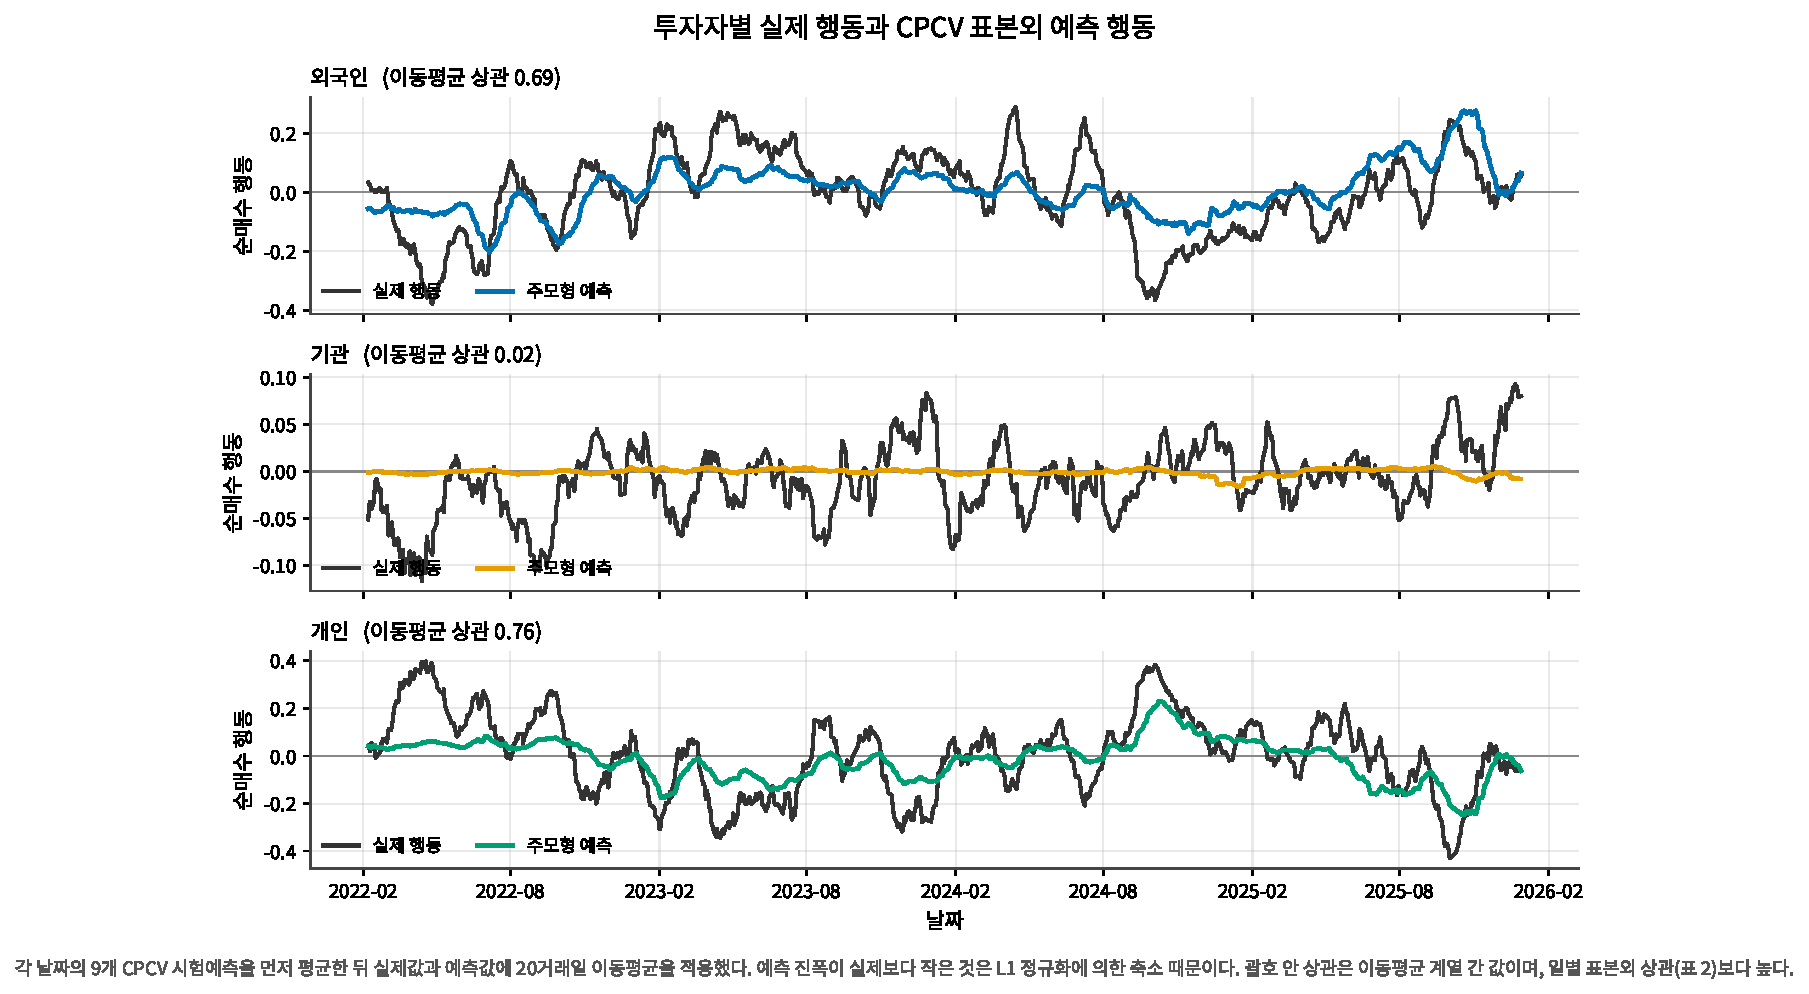
\includegraphics[width=\columnwidth]{figures/fig_actual_vs_prediction.pdf}
  \caption{실제 행동과 CPCV 표본외 예측(20거래일 이동평균). 각 날짜의 9개 시험예측을
  먼저 평균했다. 괄호 안은 평활 계열 간 상관으로,
  표~\ref{tab:performance}의 일별 상관과 직접 비교하지 않는다.}
  \Description{외국인, 기관, 개인의 실제 순매수와 모형 예측을 시간축에 겹쳐 그린
  세 개의 선그래프. 기관 패널에서 예측선이 0 근방에 평탄하게 놓여 있다.}
  \label{fig:prediction}
\end{figure}

\begin{table}[t]
  \caption{CPCV 표본외 성능(45개 분할 평균 $\pm$ 표준편차), 지속성 기준선, 그리고
  지연 자기행동을 포함한 승격 사양}
  \label{tab:performance}
  \small
  \centering
  \begin{tabular}{@{}lccc@{}}
    \toprule
    지표 & 외국인 & 기관 & 개인 \\
    \midrule
    \multicolumn{4}{@{}l}{\emph{SPR-IRL} (F1)--(F3), 주 사양}\\
    방향 정확도 & $0.636\pm0.039$ & $0.542\pm0.038$ & $0.608\pm0.044$ \\
    상관계수    & $0.278\pm0.110$ & $0.068\pm0.064$ & $0.245\pm0.118$ \\
    MAE         & $0.195\pm0.019$ & $0.094\pm0.008$ & $0.264\pm0.029$ \\
    MAE / 행동 SD & $0.759$ & $0.756$ & $0.791$ \\
    포화 비율   & $0.000$ & $0.000$ & $0.000$ \\
    \addlinespace
    \multicolumn{4}{@{}l}{\emph{지속성 기준선} ($a_{t+1}\!\leftarrow\!a_t$)}\\
    방향 정확도 & $0.642$ & $0.547$ & $0.616$ \\
    상관계수    & $0.359$ & $0.136$ & $0.311$ \\
    \addlinespace
    \multicolumn{4}{@{}l}{\emph{승격 사양} (F1)--(F3)$+u_{i,t}$, 정확해 (\S\ref{sec:beta})}\\
    \inputrows{sections/generated/tab1_rows.tex}
    \bottomrule
  \end{tabular}
\end{table}

그림~\ref{fig:prediction}에서 외국인과 개인의 예측 계열은 실제 계열의 국면 전환을
따라가지만(평활 상관 0.69, 0.76) 진폭은 작다. 이는 벌점의 산물이 아니라---외국인은
$\lambda=0$이다---설명력이 유한한 회귀의 조건부 기대가 갖는 일반적 성질이다. 표본외
$R^2$가 0.10--0.18인 예측치의 표준편차는 실제 행동 표준편차의 1/3 수준으로
축소된다. 기관의 예측 계열은 사실상 0선에 붙어 있다(0.02).

표~\ref{tab:performance}에서 세 가지가 드러난다. 첫째, 분할 간 산포가 커서 단일
분할의 수치로 유형을 비교할 수 없다. 둘째, 자명한 지속성 기준선이 방향 정확도와
상관계수에서 (F1)--(F3) 사양의 SPR-IRL을 앞선다. $a_t$는 $t$일 종가 이후 공개되므로
이는 정보상 이용 가능한 규칙이다. 셋째, 원인은 특징 집합의 설계에 있다. 행동의
자기상관이 $0.401/0.149/0.345$인데 (F1)--(F3)에는 자기 지연행동이 없다. 이 제한은
세 유형이 독립적으로 확립된 규칙성에 대응하는 특징만 공유하도록 한 선택이지 예측
성능을 위한 설계가 아니다. \textbf{지연 자기행동 $u_{i,t}$를 네 번째 특징으로 넣은
승격 사양은 세 유형 모두에서 지속성 기준선을 넘어서며(방향 정확도 $0.652/0.574/
0.629$, 표~\ref{tab:performance}), 이때 어떤 계수 부호가 살아남는지가
\S\ref{sec:beta}의 해석을 결정한다(표~\ref{tab:spec34}).} 즉 선호 복원과 수급
예측은 상이한 특징 집합을 요구하는 별개의 과제다.

모든 유형ㆍ모든 분할에서 학습 인덱스의 포화 비율이 0이므로 명제~\ref{prop:lasso}(b)의
전제가 성립하고, 제약 추정량~\eqref{eq:closs}은 무제약 Lasso와 일치한다. 승격 사양에서도
포화 비율은 45개 분할 전부 0이며 표본 전체에서 $|q|$의 최대값은 0.959다.

\subsection{복원된 구조: 모멘텀 축의 거울상과 그 식별 경계}
\label{sec:beta}

\begin{figure*}[t]
  \centering
  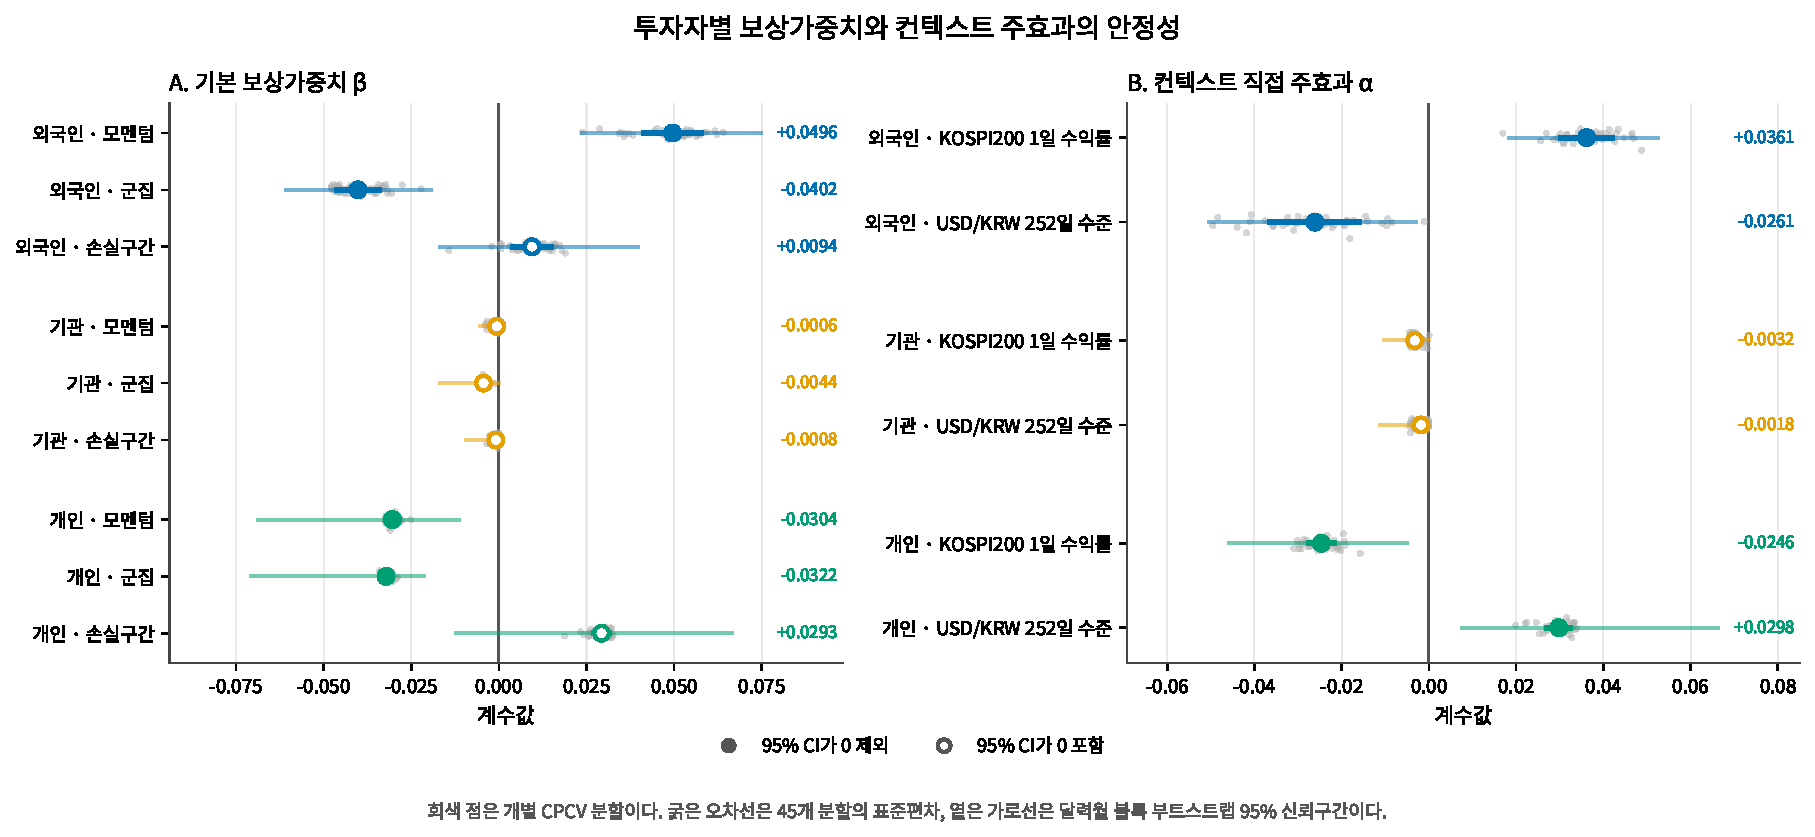
\includegraphics[width=\textwidth]{figures/fig_beta_alpha_forest.pdf}
  \caption{복원된 기본 보상가중치 $\beta$(A)와 컨텍스트 주효과 $\alpha$(B)의 안정성.
  회색 점은 45개 개별 CPCV 분할, 굵은 오차선은 분할 간 표준편차, 옅은 가로선은 달력월
  블록 부트스트랩 95\% 신뢰구간이다. 속이 빈 표식은 신뢰구간이 0을 포함하는 항이다.}
  \Description{두 패널의 forest plot. 패널 A는 세 유형의 모멘텀, 시차 교차연관,
  손실구간 계수를, 패널 B는 KOSPI200과 환율 주효과를 보인다. 외국인 모멘텀은 양,
  개인 모멘텀은 음이며 기관의 모든 표식은 속이 비어 있다.}
  \label{fig:forest}
\end{figure*}

\begin{table*}[t]
  \caption{(F1)--(F3) 주 사양과 지연 자기행동을 포함한 승격 사양의 계수 대조.
  값은 정확해 CPCV 45개 분할 평균, 괄호는 부호 일관성, CI는 달력월 블록 부트스트랩
  1{,}000회의 95\% 신뢰구간이며 $^{*}$는 0을 제외함을 뜻한다. 주 표(표~\ref{tab:performance},
  그림~\ref{fig:forest})의 Adam 수치는 변경하지 않았다.}
  \label{tab:spec34}
  \small
  \centering
  \begin{tabular}{@{}llcccc>{\raggedright\arraybackslash}p{0.14\textwidth}@{}}
    \toprule
    유형 & 항 & (F1)--(F3) 평균 & CI & 승격 사양 평균 & CI & 판정 \\
    \midrule
    \inputrows{sections/generated/tab3_body.tex}
    \bottomrule
  \end{tabular}
\end{table*}

\textbf{청산 제약이 정하는 해석의 경계.} 유형 간 계수를 비교하기 전에, 시장 청산이
기계적으로 만들 수 있는 것부터 정량화한다. 본 표본에서 외국인 순매수 1원은 평균적으로
개인 $-0.92$원, 기관 $-0.06$원, 기타 $-0.02$원으로 흡수되고, 유형별 총거래금액
비율은 $\mathbb{E}[W_{f}/W_{r}]=1.21\text{--}1.42$다. 따라서 외국인이 표준화 특징
$x$에 $\beta_f$만큼 반응하면, 개인이 아무 선호가 없어도 개인 계수에는
$\beta_{r}^{ind}\approx-0.92\times\beta_f\times(1.21\text{--}1.42)$의 성분이
유도된다(유도 과정과 가정은 부록~\ref{app:derivation}). 관측된 외국인 계수를 대입한
유도 성분은 \textbf{관측된 개인 계수를 전 항목에서 초과하거나 근사한다(관측의
84--214\%; 부록 표~\ref{tab:A2})}. 외국인만 선호를 갖는 합성 세계 1{,}000회의 전체
파이프라인 추정도 같은 결론을 준다. 개인이 물려받는 $\beta^{mom}$ 분포는
$[-0.101,-0.015]$로 관측치를 내부에 품으며, 이 세계는 동시점 상관 $-0.74$(관측
$-0.77$)와 기관의 null까지 재현한다. 반대로 선호가 전혀 없는 합성 세계에서
$\beta^{mom}$과 $\alpha$의 95\% 대역은 $\pm0.04$ 이내이므로 외국인의 $+0.0496$은 그
대역 밖(약 4.3 표준편차)에 있다. 이 두 사실이 본 절의 서술 규칙을 정한다. 유형별
계수 중 기계 대역을 초과하는 것만 선호로 읽고, 유도 범위 안의 것은 집계 수급의
구조로 읽는다.

\textbf{모멘텀 축의 거울상.} 외국인의 모멘텀 가중치는 $+0.0496$으로 45개 분할
전부에서 양수, 개인은 $-0.0304$로 전부에서 음수이며 두 부트스트랩 신뢰구간은 서로
겹치지 않고 각각 0을 제외한다(그림~\ref{fig:forest}A). 이 대비는 지연 자기행동을
통제한 승격 사양에서도 그대로 살아남는다(외국인 $+0.0331$, CI $[+0.0126,+0.0522]$;
개인 $-0.0261$, CI $[-0.0519,-0.0007]$; 표~\ref{tab:spec34}). walk-forward 10개
창에서 두 경로가 한 번도 교차하지 않으며(그림~\ref{fig:wf4}A), 벌점 종류와
$\lambda$ 통일에도 불변이다(부록 표~\ref{tab:A3}). 해석은 비대칭적이다. 외국인의
양수는 무선호 합성 대역 밖이고 자기상관ㆍ청산 통제를 모두 통과하므로 추세추종
선호로 읽으며, 이는 외국인 추세거래
문헌~\cite{grinblatt2000investment,choe1999foreign}과 부합한다. 개인의 음수는
부호와 안정성이 같은 검증을 통과하지만 크기가 청산 유도 범위 안에 있으므로,
독립적 역추세 선호의 증거로 읽지 않고 \emph{외국인의 추세거래가 청산 제약을 통해
개인 집계 수급에 남기는 반대 부호}까지만 주장한다. 개인 고유의 역추세 성향이 있는지는
이 자료의 집계 수준에서 식별되지 않는다.

\textbf{컨텍스트 주효과: 서술적 결과로 격하.} 주 사양의 $\alpha$ 네 계수(외국인
$+0.0361$/$-0.0261$, 개인 $-0.0246$/$+0.0298$)는 45개 분할 전부에서 부호가 유지되고
신뢰구간이 0을 제외한다(그림~\ref{fig:forest}B). 그러나 두 가지 이유로 본 연구는
이를 선호의 거울상이 아니라 ``관측된 집계 수급의 음의 교차 연관''이라는 서술적
결과로 제한한다. 첫째, 유도 성분이 관측을 초과한다(부록 표~\ref{tab:A2}). 둘째,
$\alpha^{KOSPI}$는 지연 자기행동을 통제하면 개인에서 $+0.0274$(45개 분할 전부 양수,
CI $[+0.0039,+0.0532]$)로 \textbf{부호가 반전}되고 외국인에서 $+0.0128$로 축소되어
CI가 0을 포함한다(표~\ref{tab:spec34}). 즉 주 사양의 개인 음수 $\alpha^{KOSPI}$는
개인 수급의 자기상관을 $\alpha$가 대신 흡수한 결과였다. $\alpha^{FX}$의 대비(외국인
$-0.0217$, 개인 $+0.0303$)만이 통제 후에도 CI를 유지하는 컨텍스트 결과다.

\textbf{유형 간 시차 교차연관.} 이 계수는 세 유형 모두 45개 분할 전부에서 음수이고
외국인($-0.0402$)과 개인($-0.0322$)은 신뢰구간도 0을 제외한다. 그러나 선호가 전혀
없는 합성 수급에서도 이 계수는 외국인 $[-0.057,-0.018]$, 개인 $[-0.085,-0.011]$로
음수가 되며 관측치는 두 대역의 내부에 있다(부록 표~\ref{tab:A2b}). 따라서 음의 시차
교차연관은 행동적 해석 없이 청산 제약과 자기상관만으로 발생 가능한 크기이며, 본
연구는 이를 서술적 결과로만 보고한다.

\textbf{손실구간.} 개인의 손실구간 가중치는 $+0.0293$으로 45개 분할 전부에서
양수이며 처분효과 문헌~\cite{shefrin1985disposition,odean1998investors}의 기준가격
의존성과 정합한다. 그러나 그림~\ref{fig:forest}A에서 보듯 세 유형 모두 신뢰구간이
0을 포함한다. 개인의 구간은 $[-0.0122,+0.0665]$로, 45개 분할에서 부호가 100\%
일관됨에도 월 블록 재표집에서는 5.5\%가 부호를 뒤집으며, 지연 자기행동을 통제하면
$+0.0115$(77.8\%)로 더 약해진다(표~\ref{tab:spec34}). 이는 CPCV 분할이 관측을
공유하기 때문에 부호 일관성이 불확실성을 과소평가한다는 \S\ref{sec:protocol}의
경고가 실제로 작동한 사례다. 따라서 처분효과와 정합하는 부호를 관측했다고 보고하되
통계적으로 확립된 결과로 주장하지 않는다.

\textbf{상호작용.} $B$ 12개는 동시에 검토한 탐색적 항목이다. 정확해 기준으로 45개
분할 부호가 유지되고 부트스트랩을 통과하는 항은 외국인
모멘텀$\times$KOSPI200($-0.0141$)과 개인 손실구간$\times$환율($-0.0408$)이다. Adam
해에서 100\% 일관으로 보였던 개인 모멘텀$\times$환율($+0.0144$)은 정확해에서
$-0.0106$(음수 91.1\%)으로 뒤집히므로 목록에서 제외한다(부록 표~\ref{tab:A1}).

\subsection{안정성}
\label{sec:stability}

\begin{figure*}[t]
  \centering
  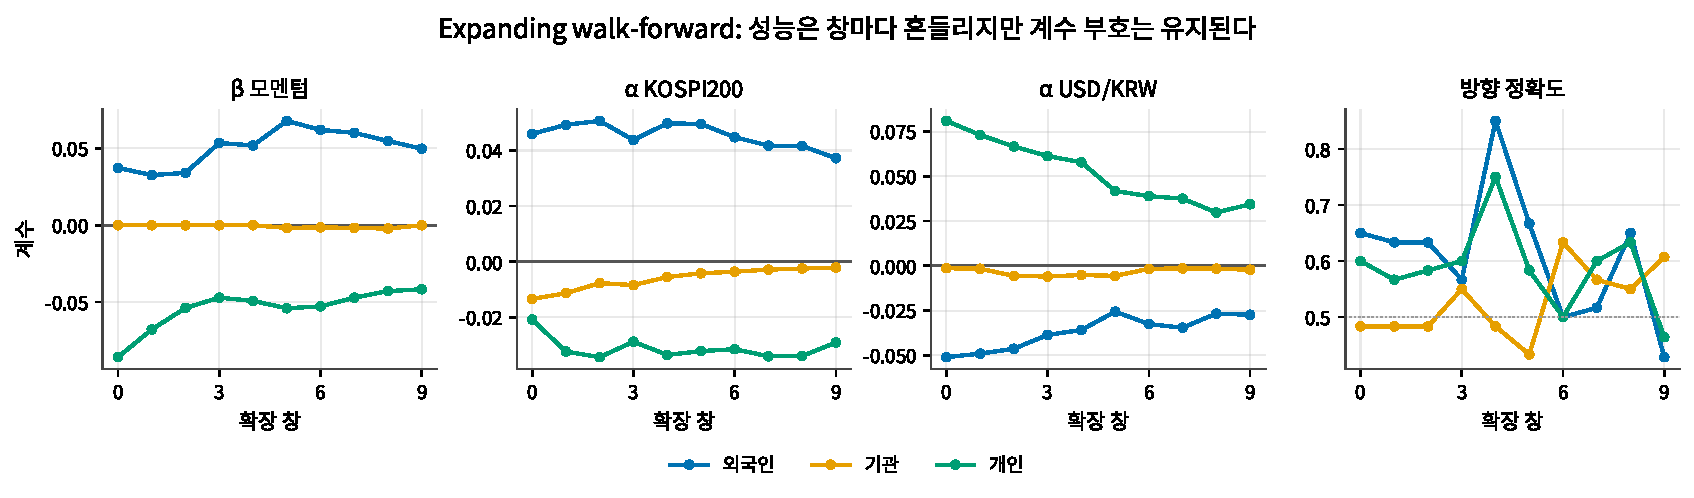
\includegraphics[width=\textwidth]{figures/fig_walk_forward.pdf}
  \caption{Expanding walk-forward 10개 창의 계수 경로와 방향 정확도((F1)--(F3) 주
  사양). 성능은 창마다 흔들리지만 계수 부호는 유지되며, 외국인과 개인의 모멘텀
  경로는 한 번도 교차하지 않는다.}
  \Description{확장 창 번호를 가로축으로 하여 세 유형의 모멘텀 계수, 두 컨텍스트
  주효과, 방향 정확도를 그린 네 개의 선그래프.}
  \label{fig:walkforward}
\end{figure*}

\begin{figure*}[t]
  \centering
  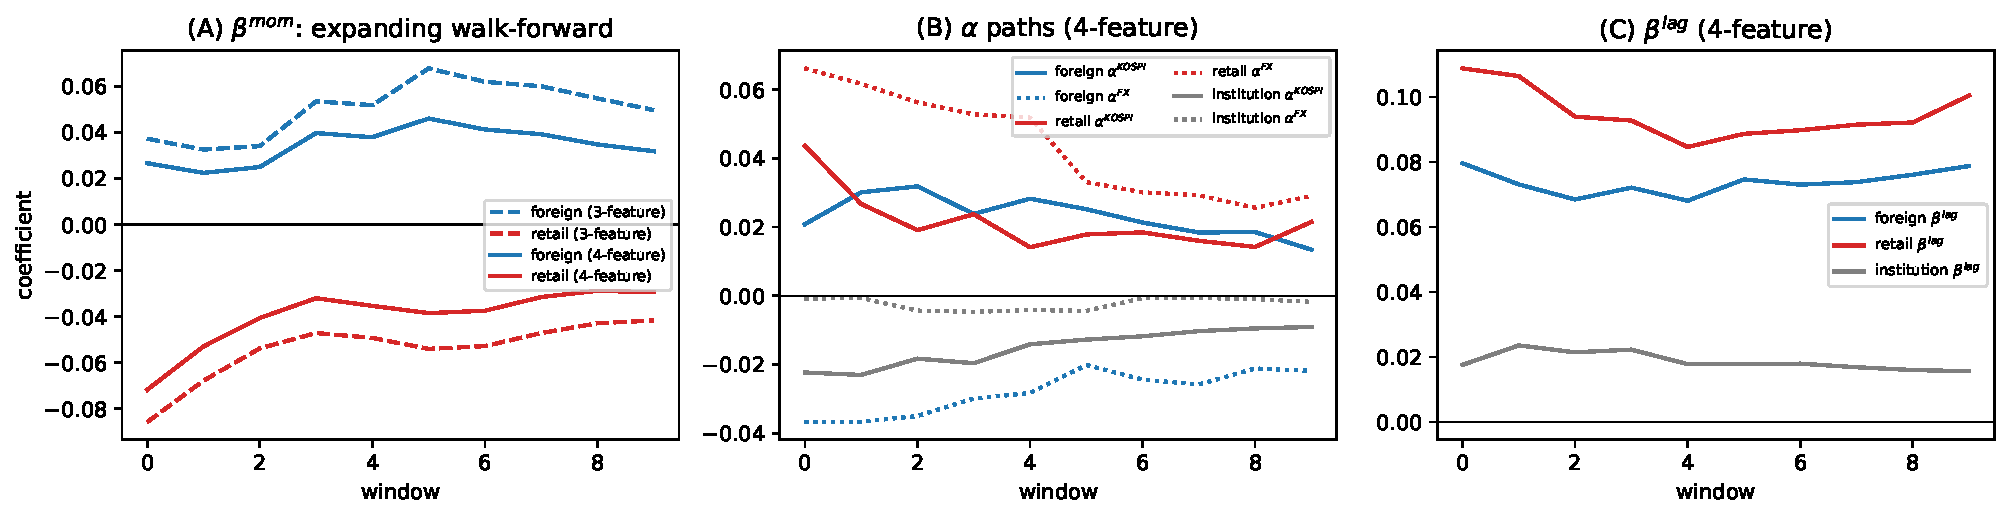
\includegraphics[width=\textwidth]{figures/fig3ext_walk_forward_4feature.pdf}
  \caption{승격 사양의 walk-forward 계수 경로(그림~\ref{fig:walkforward}의 확장).
  (A) $\beta^{mom}$: 점선은 (F1)--(F3), 실선은 승격 사양이며 두 유형의 경로가 어느
  사양에서도 교차하지 않는다. (B) 승격 사양의 $\alpha$ 경로: 개인 $\alpha^{KOSPI}$가
  10개 창 전부에서 양수다. (C) 지연 자기행동 계수 $\beta^{lag}$.}
  \Description{세 패널의 선그래프. 왼쪽 패널은 외국인과 개인의 모멘텀 계수 경로를
  3특징과 4특징 사양에 대해 각각 실선과 점선으로 보이고, 가운데 패널은 세 유형의
  KOSPI200 및 환율 주효과 경로를, 오른쪽 패널은 세 유형의 지연 자기행동 계수를
  보인다.}
  \label{fig:wf4}
\end{figure*}

\textbf{(V2)} 부트스트랩 결과는 셋으로 갈린다. 모멘텀 거울상과 컨텍스트 거울상을
이루는 8개 항이 모두 0을 제외하고, 손실구간은 통과하지 못하며, 기관은 어떤 항도
0을 제외하지 못한다(그림~\ref{fig:forest}의 속 빈 표식).

\textbf{(V3)} 그림~\ref{fig:walkforward}에서 성능은 크게 흔들린다. 외국인 방향
정확도는 0.43--0.85를 오가며 평균 $0.610\pm0.116$, 상관은 $0.131\pm0.162$로 CPCV의
0.278에서 절반 이하다. CPCV는 시험 폴드를 학습 폴드보다 앞세울 수 있는 반면
walk-forward는 그렇지 않으므로, 본 연구는 이 저하를 시간 구조에서 오는 일반화
한계로 그대로 보고한다. 반면 계수 경로는 흔들리지 않는다. 외국인 모멘텀은 10개 창
전부 양수, 개인은 전부 음수이며 두 경로가 한 번도 교차하지 않고, 두 컨텍스트
주효과에서도 같은 거울상이 유지된다. 기관의 경로는 0선에 붙어 있다.

\textbf{(V4)} 외국인과 개인의 계수는 $L_1$, $L_2$, 무벌점에서 소수점 넷째 자리까지
일치하므로 거울상은 벌점의 산물이 아니다. 반면 기관의 계수만 벌점에 따라
이동한다(시차 교차연관 $-0.0076\rightarrow-0.0124$, 손실구간
$-0.0000\rightarrow-0.0018$).

\textbf{승격 사양의 검증.} 지연 자기행동을 포함한 사양에도 V1--V4를 동일하게
적용했다(표~\ref{tab:spec34}, 그림~\ref{fig:wf4}). 모멘텀 대비와 $\alpha^{FX}$
대비는 네 검증을 모두 통과하고(walk-forward 10/10 창 부호 유지, 경로 비교차),
$\alpha^{KOSPI}$는 개인에서 10개 창 전부 양수로 반전되며, 손실구간은 약화된다.
외국인ㆍ개인 계수가 $L_1$/$L_2$/무벌점에서 소수 넷째 자리까지 일치하고 기관만
이동하는 패턴도 주 사양과 동일하다. 지연 자기행동을 컨텍스트와 상호작용시킨 확장
사양에서는 해당 상호작용 6개 항 전부의 CI가 0을 포함하며 다른 항의 변화는 0.0015
이내이므로, 본문은 파라미터 절약을 위해 $\beta$ㆍ$\alpha$만 확장한 사양을 보고한다.

\subsection{기관: 수렴된 null}
\label{sec:null}

기관 수급에 대해 SPR-IRL은 일별 빈도에서 안정적으로 식별되는 선호를 찾지 못했고,
본 연구는 이를 은폐하지 않고 결과로 보고한다. 근거는 다섯이다. (i) 예측 계열이 0선에
퇴화한다(그림~\ref{fig:prediction}). (ii) 시차 교차연관을 제외한 계수의 크기가 다른
유형보다 한 자릿수 이상 작다---현행 $\lambda$에서 $-0.0006$ㆍ$-0.0008$(약 $1/40$),
$\lambda$를 0으로 통일해도 $-0.0029$ㆍ$-0.0018$(약 $1/15$--$1/20$; 부록
표~\ref{tab:A3}). (iii) 부트스트랩에서 0을 제외하는 항이 없다(그림~\ref{fig:forest}).
(iv) 계수가 벌점 선택에 좌우된다. (v) walk-forward 10개 창에서 모멘텀 부호 일관성이
40\%, 손실구간이 0\%다.

\textbf{이 null은 최적화 실패가 아니다.} 명제~\ref{prop:lasso}에 따라 기관의 학습
인덱스에서 제약 문제~\eqref{eq:closs}은 볼록이고 그 해가 유일하다. 도달한 해와 동일
목적함수의 폐쇄형 최적해를 비교하면 기관의 목적함수 상대 격차는 평균 0.17\%, 최대
0.48\%에 불과하다(외국인 0.21\%, 개인 0.92\%). 세 유형 모두 도달 가능한 최적해에
근접했고, 기관에서만 그 최적해의 계수가 0 근방이다. 데이터가 기관에 대해 결정하는
선호가 없는 것이지 최적화가 찾지 못한 것이 아니다. 이 벌점 의존성은 계수 수준에서도
확인된다. 기관의 모멘텀ㆍ손실구간 좌표에서 목적함수 상대 격차 0.2\% 이내의 두
해---보고된 확률적 해와 폐쇄형 해---가 각각 $-0.0006$ㆍ$-0.0008$과 정확히 0(45개
분할 중 36개ㆍ44개)을 주므로, 이 좌표들에서 목적함수는 사실상 평평하며 0이 아닌
잔여값과 그로부터 계산된 부호 일관성(71\%ㆍ80\%)은 신호가 아니라 최적화
잔여물이다(부록 표~\ref{tab:A1}).

경제적으로 이 null은 투자자 분류에 대한 발견으로 읽어야 한다. ``기관''은 연기금,
투신, 보험, 사모, 금융투자를 합산한 범주다. 이 범주의 일평균 총거래금액은 958억
원으로 세 유형 중 가장 크지만 순매수 강도의 표준편차는 0.125로 가장 작다---큰
총거래가 반대 방향으로 상쇄되고 있다는 직접적 흔적이다. 상이한 목적함수를 가진 세부
주체들의 수급을 합산하면 일별 빈도에서 식별되는 공통 선호가 남지 않는다는 것이 본
결과의 내용이며, 세부 주체 분해는 \S\ref{sec:future}의 검정 가능한 가설로 남긴다.

다만 이 null은 특징 공간에 한정된다. 지연 자기행동을 통제한 승격 사양에서 기관은
$\alpha^{KOSPI}=-0.0113$(45개 분할 전부 음수, CI $[-0.0209,-0.0031]$)과 자기지연
$+0.0175$를 보이므로(표~\ref{tab:spec34}), ``어떤 항도 부트스트랩을 통과하지
못한다''는 서술은 (F1)--(F3) 주 사양에 한정해 유지한다.

\subsection{구성 타당성 점검}
\label{sec:construct}

\begin{table}[t]
  \caption{사전 부호 기대와 복원 결과}
  \label{tab:construct}
  \small
  \begin{tabular}{@{}>{\raggedright\arraybackslash}p{0.30\columnwidth}
                  >{\raggedright\arraybackslash}p{0.13\columnwidth}
                  >{\raggedright\arraybackslash}p{0.26\columnwidth}
                  >{\raggedright\arraybackslash}p{0.16\columnwidth}@{}}
    \toprule
    규칙성 & 사전 기대 & 복원 결과 & 판정 \\
    \midrule
    외국인 추세거래~\cite{grinblatt2000investment,choe1999foreign}
      & $\beta^{mom}\!>\!0$ & $+0.0496$ (100\%, CI 0 제외) & 부합 \\
    개인 역추세~\cite{grinblatt2000investment,kaniel2008individual}
      & $\beta^{mom}\!<\!0$ & $-0.0304$ (100\%, CI 0 제외) & 부합, 단 청산 유도 범위 내 \\
    처분효과~\cite{shefrin1985disposition,odean1998investors}
      & $\beta^{uw}\!>\!0$ & $+0.0293$ (100\%, CI 0 포함) & 부분 부합 \\
    기관 시차 교차연관 (참조:~\cite{lakonishok1992impact})
      & $\beta^{herd}\!>\!0$ & $-0.0044$ (100\%, CI 0 포함) & 측정 대상 상이 \\
    \bottomrule
  \end{tabular}
\end{table}

표~\ref{tab:construct}이 대조 결과다. 동일한 특징과 모형 형태를 부여하고 파라미터만
분리 학습했음에도 복원된 부호가 독립적으로 확립된 규칙성과 부합하고 두 유형이
모멘텀에서 정반대로 갈린다는 점이 구성 타당성의 증거다. 마지막 행은 측정 대상이
다르기 때문에 불일치로 보인다. Lakonishok 외~\cite{lakonishok1992impact}는 기관
\emph{내부}의 군집을, 식~\eqref{eq:herd}은 기관이 \emph{다른 두 유형}과 같은 방향으로
움직이는지를 측정하므로 본 결과는 해당 문헌의 반증이 아니다. 나아가
\S\ref{sec:beta}의 합성 실험은 음의 시차 교차연관이 선호 없이 청산 제약만으로
발생함을 보이므로, 이 항목은 구성 타당성 대조가 아니라 식별 경계의 예시로 읽는 것이
옳다.

%  의존:  sections/generated/*.tex (scripts/revision_20260727_make_tex_tables.py 산출)
% =====================================================================

\section{방법: SPR-IRL}
\label{sec:method}

본 절은 대칭 선호복원(Symmetric Preference Recovery, 이하 SPR-IRL) 절차를
정의한다. SPR-IRL은 모형 하나가 아니라 (i) 공유 특징 위의 대칭 추정, (ii) 표본외
안정성 평가, (iii) 사전 부호 기대와의 대조로 이루어진 절차다.

\subsection{연속 행동과 대칭 추정}
\label{sec:setup}

투자자 유형을 $\mathcal{I}=\{\text{외국인},\text{기관},\text{개인}\}$으로 둔다.
유형 $i$의 $t$일 총매수ㆍ총매도금액을 $V^{buy}_{i,t}$, $V^{sell}_{i,t}$라 하면
행동을
\begin{equation}
u_{i,t}=\frac{V^{buy}_{i,t}-V^{sell}_{i,t}}
             {V^{buy}_{i,t}+V^{sell}_{i,t}}\in[-1,1]
\label{eq:action}
\end{equation}
로 정의한다. 분모가 시장 전체가 아니라 해당 유형의 총거래금액이므로 $u_{i,t}$는
유형별 거래 규모에 영향받지 않는 공통 척도가 되며, 이진 라벨과 달리 강도 정보를
보존한다.

세 유형은 동일한 상태 특징 $x_{i,t}\in\mathbb{R}^{3}$, 동일한 컨텍스트
$C_t\in\mathbb{R}^{2}$, 동일한 모형 형태를 부여받고 파라미터
$\theta_i=(\beta_i,B_i,\alpha_i)$만 각자의 데이터로 분리 학습한다. 유형별로 다른
특징을 미리 배정하지 않으므로, 결과의 유형 간 차이는 설계가 아니라 데이터에서
학습된 것이며 이것이 계수의 직접 비교를 정당화한다.

학습 표본은 $(x_{i,t},C_t,a_{i,t+1})$, $a_{i,t+1}=u_{i,t+1}$이다. $t$일 상태가
$t+1$일 행동을 설명하므로 미래 거래는 특징에 들어가지 않는다.

\subsection{보상 특징과 시장 컨텍스트}
\label{sec:features}

세 특징과 두 컨텍스트는 모두 각 분할의 학습 인덱스에서만 표준화하므로, 이후 계수는
1표준편차 변화의 효과로 읽는다.

\textbf{(F1) 중기 모멘텀} $x^{mom}_{t}=\log(P_t/P_{t-20})$. 20거래일은 해석을 위한
사전 지정값이며 자료에서 최적화하지 않았다. 양수는 추세추종, 음수는 역추세를 뜻하고
부호 기대는 유형별 모멘텀 거래 문헌~\cite{grinblatt2000investment,choe1999foreign}에서
온다. 이 창과 (F3)의 망각계수 $\rho=0.98$은 사전 지정값이며,
$\rho\in\{0.95,0.98,0.99\}\times$창$\in\{10,20,60\}$의 아홉 조합 전부에서
\S\ref{sec:beta}의 모멘텀 부호 대비와 개인 손실구간 부호가 유지된다(부록
표~\ref{tab:A4}).

\textbf{(F2) 유형 간 시차 교차연관} 유형 $i$를 제외한 두 유형의 전일 행동 횡단면
평균
\begin{equation}
x^{herd}_{i,t}=\tfrac{1}{2}\left(u_{j,t-1}+u_{k,t-1}\right),\qquad j,k\neq i.
\label{eq:herd}
\end{equation}
1거래일 지연은 정보 제약이 아니라, 동일 거래일 유형 간 수급의 회계적 상쇄를 예측
변수에서 배제하기 위한 설계 선택이다(\S\ref{sec:beta}). 부호 기대는 기관 군집행동
문헌~\cite{lakonishok1992impact}을 참조하되, 해당 문헌은 기관 \emph{내부}의 군집을,
식~\eqref{eq:herd}은 \emph{유형 간} 시차 관계를 측정하므로 이 특징의 계수는
군집행동의 직접 검정이 아니다(\S\ref{sec:construct}).

\textbf{(F3) 평균단가 대비 손실구간} 평균단가 대용치 $\bar P_{i,t}$와 당일 총거래
VWAP $P^{vwap}_{i,t}$로
\begin{equation}
x^{uw}_{i,t}=\max\!\left(
\frac{\bar P_{i,t}-P^{vwap}_{i,t}}{\bar P_{i,t}},\,0\right).
\label{eq:underwater}
\end{equation}
0에서 절단하므로 이 변수는 준거점 의존적 설계다. 평균단가는 총매수ㆍ총매도 수량과
금액으로 유효 보유량을 재귀 갱신해 구하되 전일 보유량에 망각계수 $\rho=0.98$을
곱한다(반감기 약 34거래일). 부호 기대는 처분효과
문헌~\cite{shefrin1985disposition,odean1998investors}에서 온다. 다만 이 대용치는
집계 거래로 만든 근사치이므로 $x^{uw}$의 계수를 처분효과의 직접 검정으로 읽을 수
없다.

\textbf{컨텍스트}는 KOSPI200 1일 수익률 $r_t$와 원/달러 환율 수준
$z_t=(\log e_t-\mu_{t-1,252})/\sigma_{t-1,252}$이다. 평균과 표준편차는 $t-1$까지의
252거래일만 쓴다. 삼성전자의 KOSPI200 비중 때문에 종목 모멘텀과 시장수익률이
겹치며 특징--컨텍스트 상관은 $-0.29$에서 $0.22$ 범위다. 따라서 개별 계수는 다른
항이 통제된 조건부 연관이다.

\subsection{근시안적 보상과 제약 Lasso로의 환원}
\label{sec:model}

유형 $i$의 행동점수를
\begin{equation}
q_{i,t}=(\beta_i+B_iC_t)^{\top}x_{i,t}+\alpha_i^{\top}C_t
\label{eq:score}
\end{equation}
로 둔다. $\alpha$는 종목 특징이 평균일 때도 행동 수준을 옮기는 수준효과, $B$는
컨텍스트에 따라 특징 민감도가 달라지는 기울기 효과다. 상호작용을 넣으면서 하위차수
항 $C_t$를 빼는 것은 표준적 사양 오류이므로 $\alpha$의 포함은 자료로 정당화할
대상이 아니다. 연속 행동에 대한 단기 보상을
$R_i=q_{i,t}a-\tfrac{\kappa}{2}a^{2}$로 두면 최적 정책은
\begin{equation}
a^{*}_{i,t+1}=\mathrm{clip}(q_{i,t}/\kappa,-1,1)
\label{eq:policy}
\end{equation}
이다. 이차항이 없으면 해가 거의 항상 $\pm1$이 되어 행동 강도를 재현할 수 없다.
$\kappa$는 식별을 위해 1로 고정하며, 이는 보상과 계수의 단위를 고정하는 정규화이지
곡률이 경험적으로 1이라는 주장이 아니다. 학습목적은
\begin{equation}
\min_{\theta_i}\ \frac{1}{|\mathcal{D}_i|}
\sum_{t\in\mathcal{D}_i}\!\bigl(a^{*}_{i,t+1}-a_{i,t+1}\bigr)^{2}
+\lambda_i\lVert\theta_i\rVert_1
\label{eq:loss}
\end{equation}
이다. 여기서
\[
\begin{aligned}
z_{i,t}&=[\,x_{i,t};\ \mathrm{vec}(x_{i,t}C_t^{\top});\ C_t\,]\in\mathbb{R}^{11},\\
\theta_i&=[\,\beta_i;\ \mathrm{vec}(B_i);\ \alpha_i\,]
\end{aligned}
\]
로 두면 $q_{i,t}=\theta_i^{\top}z_{i,t}$이므로 식~\eqref{eq:loss}은 $z$ 위의 벌점 회귀
형태를 갖는다.

\textbf{그러나 식~\eqref{eq:loss}은 볼록이 아니다.} 예측값이 절단되기 때문이다.
한 관측의 손실을
$\ell(u)=(\mathrm{clip}(u)-a)^2$라 하자. $a=0$이면
$\ell(-2)=\ell(-1)=1$, $\ell(0)=0$이므로
$\ell(-1)$이 두 값의 평균 $0.5$를 넘어 $\ell$은 볼록이 아니다. 더구나 $\mathrm{clip}$은 상자
$[-1,1]^{n}$으로의 사영이고 관측 행동이 그 상자 안에 있으므로 모든 $\theta$에서
\[
\lVert\mathrm{clip}(Z\theta)-a\rVert\ \le\ \lVert Z\theta-a\rVert
\]
가 성립한다. 즉 포화는 오차를 줄일 수도 있으며(부록~\ref{app:convexity}의 최소 예),
어떤 해에서 $|q|<1$임을 확인하는 것만으로 포화영역에 더 좋은 해가 없다고 결론지을 수
없다.

따라서 본 논문은 추정량을 처음부터 제약 문제로 정의한다. 학습 인덱스
$\mathcal{D}_i$에 대해 $\mathcal{C}_i=\{\theta:\ |z_{i,t}^{\top}\theta|\le 1,\
\forall t\in\mathcal{D}_i\}$로 두고
\begin{equation}
\hat\theta_i=\operatorname*{arg\,min}_{\theta\in\mathcal{C}_i}\ \frac{1}{|\mathcal{D}_i|}
\sum_{t\in\mathcal{D}_i}\bigl(z_{i,t}^{\top}\theta-a_{i,t+1}\bigr)^{2}
+\lambda_i\lVert\theta\rVert_1 .
\label{eq:closs}
\end{equation}
이 제약은 계산상의 편의가 아니라 식별 제약이다. 포화영역에서는
$\theta\mapsto\mathrm{clip}(Z\theta)$가 단사가 아니어서---모든 관측이 포화된 $\theta$는
$c>1$배 해도 예측이 같다---파라미터가 식별되지 않으며, $\lambda=0$이면 그 영역의
최적해는 연속체를 이룬다. $\mathcal{C}_i$는 정책이 내부해인 영역, 곧 계수를 행동 강도의
1표준편차 효과로 읽을 수 있는 영역이다.

\begin{proposition}[제약 Lasso 환원과 유일성]
\label{prop:lasso}
(a) $\mathcal{C}_i$ 위에서 식~\eqref{eq:loss}과 식~\eqref{eq:closs}의 목적식은 동일하다.
(b) 무제약 Lasso 해 $\tilde\theta_i$가 $\mathcal{C}_i$에 속하면 $\tilde\theta_i$는
식~\eqref{eq:closs}의 전역해이며, $\mathcal{C}_i$의 \emph{내부}에 속하면 두 문제의 KKT
조건이 일치한다(제약 승수가 0). (c) 식~\eqref{eq:closs}은 볼록 다면체 위의 볼록 문제이고,
$\lambda_i=0$일 때 $\mathrm{rank}(Z_i)=p$이면, $\lambda_i>0$일 때 등상관 집합
$E=\{j:|\tfrac{2}{n}z_{j}^{\top}(a-Z\hat\theta)|=\lambda_i\}$에 대해
$\mathrm{rank}(Z_{i,E})=|E|$이면 그 해는 유일하다.
\end{proposition}

증명은 부록~\ref{app:convexity}에 있다. 본 표본에서 세 조건이 모두 성립한다. 45개
분할$\times$3유형 전부에서 학습 인덱스의 $\max_t|z_t^{\top}\hat\theta|$가 0.558을 넘지
않아 해는 $\mathcal{C}_i$의 내부에 있고, $\mathrm{rank}(Z)=11$(최악 조건수 6.86)이며,
$\lambda>0$인 두 유형에서 $\mathrm{rank}(Z_E)=|E|$다(부록 표~\ref{tab:F1}). 따라서
식~\eqref{eq:closs}의 해는 존재하고 유일하며 무제약 Lasso 해와 일치한다. 이 영역
안에서 SPR-IRL의 ``선호를 복원한다''와 ``수급을 회귀한다''는 수치적으로 구별되지
않으며, 문제가 볼록이므로 좌표하강 정확해로 직접 풀 수 있다. 본 개정에서 보고하는
모든 확장 사양은 이 정확해로 추정했다(\S\ref{sec:null}, 부록 표~\ref{tab:A1}).

무제약 문제~\eqref{eq:loss}의 전역 최적성은 이와 별개이며 본 논문은 그것을 주장하지
않는다. 다만 부록~\ref{app:convexity}는 두 가지를 보고한다. 첫째, $\hat\theta$보다 나은
목적값을 갖는 어떤 $\theta$도 학습 관측의 20.7\%(외국인)ㆍ4.2\%(기관)ㆍ40.2\%(개인)를
넘게 포화시킬 수 없다는 증명 가능한 경계. 둘째, 분할ㆍ유형당 939개, 합계 42{,}255개
시작점의 다중시작 탐색에서 더 나은 해가 하나도 발견되지 않았다는 사실이다.

이 일치는 결함이 아니라 근시안 가정의 귀결이다. 한 걸음만 내다보면 오늘의 행동이
내일 이후에 영향을 주지 않으므로, 무엇을 원하는가(보상)와 무엇을 하는가(정책)가
하나로 겹친다. 최대엔트로피 IRL~\cite{ziebart2008maximum}의
$\pi\propto\exp(R/\tau)$를 적용하면 $\pi$는 평균 $q$의 절단정규분포가 되어
점추정치가 위와 일치하므로, 이 환원은 특정 구현의 우연이 아니라 근시안ㆍ이차보상
설정 전반의 성질이다. 역강화학습 정식화의 가치는 확장 경로에 있다. 상태 동역학과
다기간 가치를 넣는 순간 보상은 정책과 갈라지고 회귀로는 도달할 수 없는 구조적
복원이 된다(\S\ref{sec:discussion}).

\subsection{검증 프로토콜}
\label{sec:protocol}

복원된 계수를 그대로 보고하지 않고 네 단계를 거친다. \textbf{(V1)} 10개 시간 폴드
중 2개를 시험으로 쓰는 조합형 정화 교차검증~\cite{lopez2018advances}으로
$\binom{10}{2}=45$개 분할을 만들고, 1일 purge와 5일 embargo를 적용하며 모든
표준화는 학습 인덱스에만 적합한다. 분할들이 관측을 공유하므로 부호 일관성은
$p$-값이 아니라 안정성 지표로만 해석한다. \textbf{(V2)} 그 한계를 보완하기 위해
표본을 달력월 블록으로 나누어 1{,}000회 복원추출하고 95\% 신뢰구간을 구한다. 월
블록은 일별 수급의 자기상관을 블록 안에 보존한다. \textbf{(V3)} CPCV는 시험 폴드가
학습 폴드보다 앞설 수 있으므로, 최초 400개 관측에서 시작해 5일 purge 후 다음
60거래일을 예측하고 학습 구간을 60거래일씩 넓히는 expanding walk-forward를 10개 창
수행한다. \textbf{(V4)} 결과가 $L_1$ 벌점의 산물이 아님을 보이기 위해 $L_2$ 및
무벌점으로 재추정해 부호를 비교한다.

지표는 MAE, RMSE, 방향 정확도($\mathrm{sign}(a^{*})=\mathrm{sign}(a)$의 비율),
예측--실제 상관, 포화 비율이다. 유형 간 행동 표준편차가 다르므로 오차의 절대값은
유형 간 비교에 쓰지 않는다. 자명한 참조로 전일 자기행동을 그대로 예측하는 지속성
규칙을 함께 보고한다.

% =====================================================================
\section{실험}
\label{sec:experiments}

\subsection{데이터}
\label{sec:data}

삼성전자(005930) 일별 자료에서 252일 환율 이력, 20일 모멘텀, 다음 날 행동을 모두
계산할 수 있는 최신 973행을 사용한다. 상태일은 2022-01-06--2025-12-29이다. 단일
종목은 표본의 한계가 아니라 종목 고정효과와 유동성 차이를 배제하고 유형 간 선호
이질성만 분리하기 위한 통제된 설정이다.

행동 평균은 세 유형 모두 0에 가깝지만 표준편차는 개인 0.334, 외국인 0.257, 기관
0.125로 다르고, 1차 자기상관은 각각 0.345, 0.401, 0.149다. 동일 거래일 유형 간
행동은 강한 음의 관계를 갖는다(외국인--개인 $-0.772$, 기관--개인 $-0.499$). 이 음의
동시점 구조가 유형 간 계수 해석에 부과하는 식별 경계는 \S\ref{sec:beta}에서
정량화한다. 세 유형 순매수 합계와 시장 전체의 차이(기타법인ㆍ기타외국인 등)는
일평균 144억 원, 거래대금의 1.3\%에 그친다.

학습 설정은 유형별로 외국인 75 epochs / batch 256 / lr 0.001 / $\lambda=0$, 기관
10 / 2048 / 0.0005 / 0.01, 개인 20 / 512 / 0.001 / 0.0003이며 seed 42, $\kappa=1$,
유형당 파라미터 11개($\beta$ 3, $B$ 6, $\alpha$ 2)다. 유형별 $\lambda$는 본
사양에서 중첩 교차검증으로 선택된 값이 아니라, 선행 이산행동 사양에서 CPCV 정확도
그리드 탐색으로 정해져 이월된 값이다. 따라서 $\lambda$ 비대칭이 결과를 만드는지
확인하기 위해 세 유형에 동일한 $\lambda\in\{0,0.0005,0.01\}$을 부여한 재추정을 부록
표~\ref{tab:A3}에 함께 보고하며, 거울상 부호는 모든 $\lambda$ 사양에서 유지된다.

\subsection{표본외 행동 재현}
\label{sec:oos}

\begin{figure}[t]
  \centering
  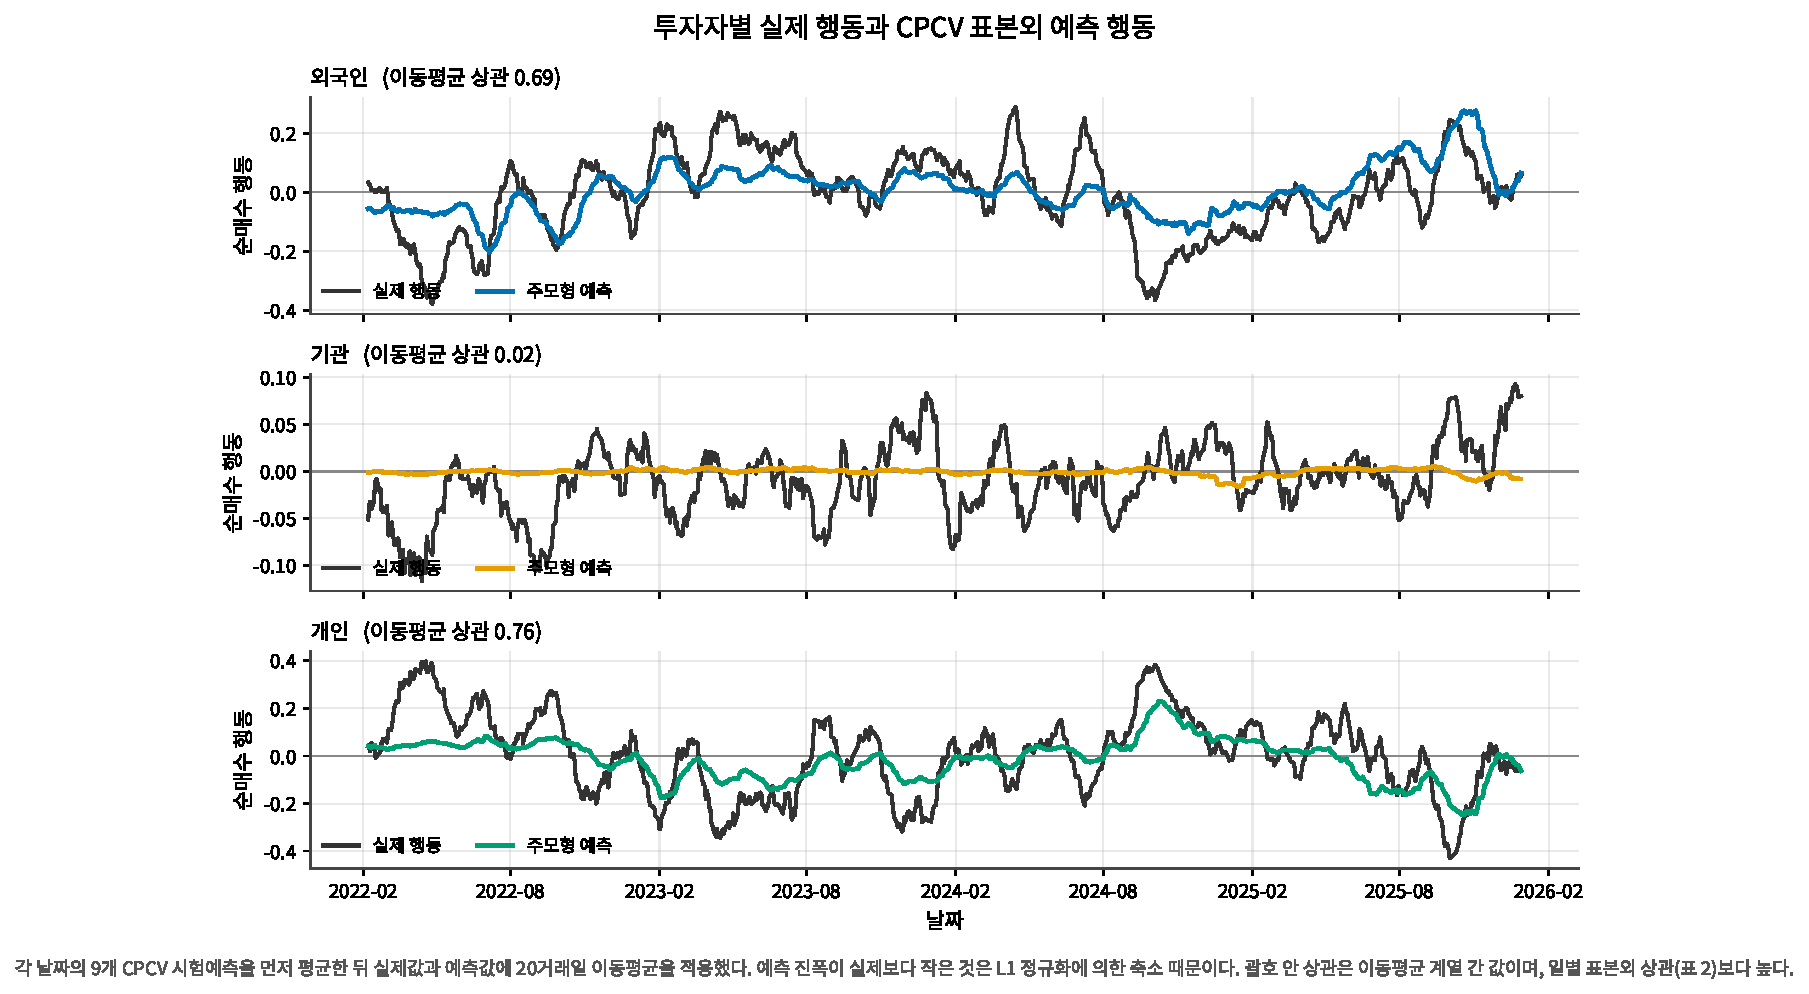
\includegraphics[width=\columnwidth]{figures/fig_actual_vs_prediction.pdf}
  \caption{실제 행동과 CPCV 표본외 예측(20거래일 이동평균). 각 날짜의 9개 시험예측을
  먼저 평균했다. 괄호 안은 평활 계열 간 상관으로,
  표~\ref{tab:performance}의 일별 상관과 직접 비교하지 않는다.}
  \Description{외국인, 기관, 개인의 실제 순매수와 모형 예측을 시간축에 겹쳐 그린
  세 개의 선그래프. 기관 패널에서 예측선이 0 근방에 평탄하게 놓여 있다.}
  \label{fig:prediction}
\end{figure}

\begin{table}[t]
  \caption{CPCV 표본외 성능(45개 분할 평균 $\pm$ 표준편차), 지속성 기준선, 그리고
  지연 자기행동을 포함한 승격 사양}
  \label{tab:performance}
  \small
  \centering
  \begin{tabular}{@{}lccc@{}}
    \toprule
    지표 & 외국인 & 기관 & 개인 \\
    \midrule
    \multicolumn{4}{@{}l}{\emph{SPR-IRL} (F1)--(F3), 주 사양}\\
    방향 정확도 & $0.636\pm0.039$ & $0.542\pm0.038$ & $0.608\pm0.044$ \\
    상관계수    & $0.278\pm0.110$ & $0.068\pm0.064$ & $0.245\pm0.118$ \\
    MAE         & $0.195\pm0.019$ & $0.094\pm0.008$ & $0.264\pm0.029$ \\
    MAE / 행동 SD & $0.759$ & $0.756$ & $0.791$ \\
    포화 비율   & $0.000$ & $0.000$ & $0.000$ \\
    \addlinespace
    \multicolumn{4}{@{}l}{\emph{지속성 기준선} ($a_{t+1}\!\leftarrow\!a_t$)}\\
    방향 정확도 & $0.642$ & $0.547$ & $0.616$ \\
    상관계수    & $0.359$ & $0.136$ & $0.311$ \\
    \addlinespace
    \multicolumn{4}{@{}l}{\emph{승격 사양} (F1)--(F3)$+u_{i,t}$, 정확해 (\S\ref{sec:beta})}\\
    \inputrows{sections/generated/tab1_rows.tex}
    \bottomrule
  \end{tabular}
\end{table}

그림~\ref{fig:prediction}에서 외국인과 개인의 예측 계열은 실제 계열의 국면 전환을
따라가지만(평활 상관 0.69, 0.76) 진폭은 작다. 이는 벌점의 산물이 아니라---외국인은
$\lambda=0$이다---설명력이 유한한 회귀의 조건부 기대가 갖는 일반적 성질이다. 표본외
$R^2$가 0.10--0.18인 예측치의 표준편차는 실제 행동 표준편차의 1/3 수준으로
축소된다. 기관의 예측 계열은 사실상 0선에 붙어 있다(0.02).

표~\ref{tab:performance}에서 세 가지가 드러난다. 첫째, 분할 간 산포가 커서 단일
분할의 수치로 유형을 비교할 수 없다. 둘째, 자명한 지속성 기준선이 방향 정확도와
상관계수에서 (F1)--(F3) 사양의 SPR-IRL을 앞선다. $a_t$는 $t$일 종가 이후 공개되므로
이는 정보상 이용 가능한 규칙이다. 셋째, 원인은 특징 집합의 설계에 있다. 행동의
자기상관이 $0.401/0.149/0.345$인데 (F1)--(F3)에는 자기 지연행동이 없다. 이 제한은
세 유형이 독립적으로 확립된 규칙성에 대응하는 특징만 공유하도록 한 선택이지 예측
성능을 위한 설계가 아니다. \textbf{지연 자기행동 $u_{i,t}$를 네 번째 특징으로 넣은
승격 사양은 세 유형 모두에서 지속성 기준선을 넘어서며(방향 정확도 $0.652/0.574/
0.629$, 표~\ref{tab:performance}), 이때 어떤 계수 부호가 살아남는지가
\S\ref{sec:beta}의 해석을 결정한다(표~\ref{tab:spec34}).} 즉 선호 복원과 수급
예측은 상이한 특징 집합을 요구하는 별개의 과제다.

모든 유형ㆍ모든 분할에서 학습 인덱스의 포화 비율이 0이므로 명제~\ref{prop:lasso}(b)의
전제가 성립하고, 제약 추정량~\eqref{eq:closs}은 무제약 Lasso와 일치한다. 승격 사양에서도
포화 비율은 45개 분할 전부 0이며 표본 전체에서 $|q|$의 최대값은 0.959다.

\subsection{복원된 구조: 모멘텀 축의 거울상과 그 식별 경계}
\label{sec:beta}

\begin{figure*}[t]
  \centering
  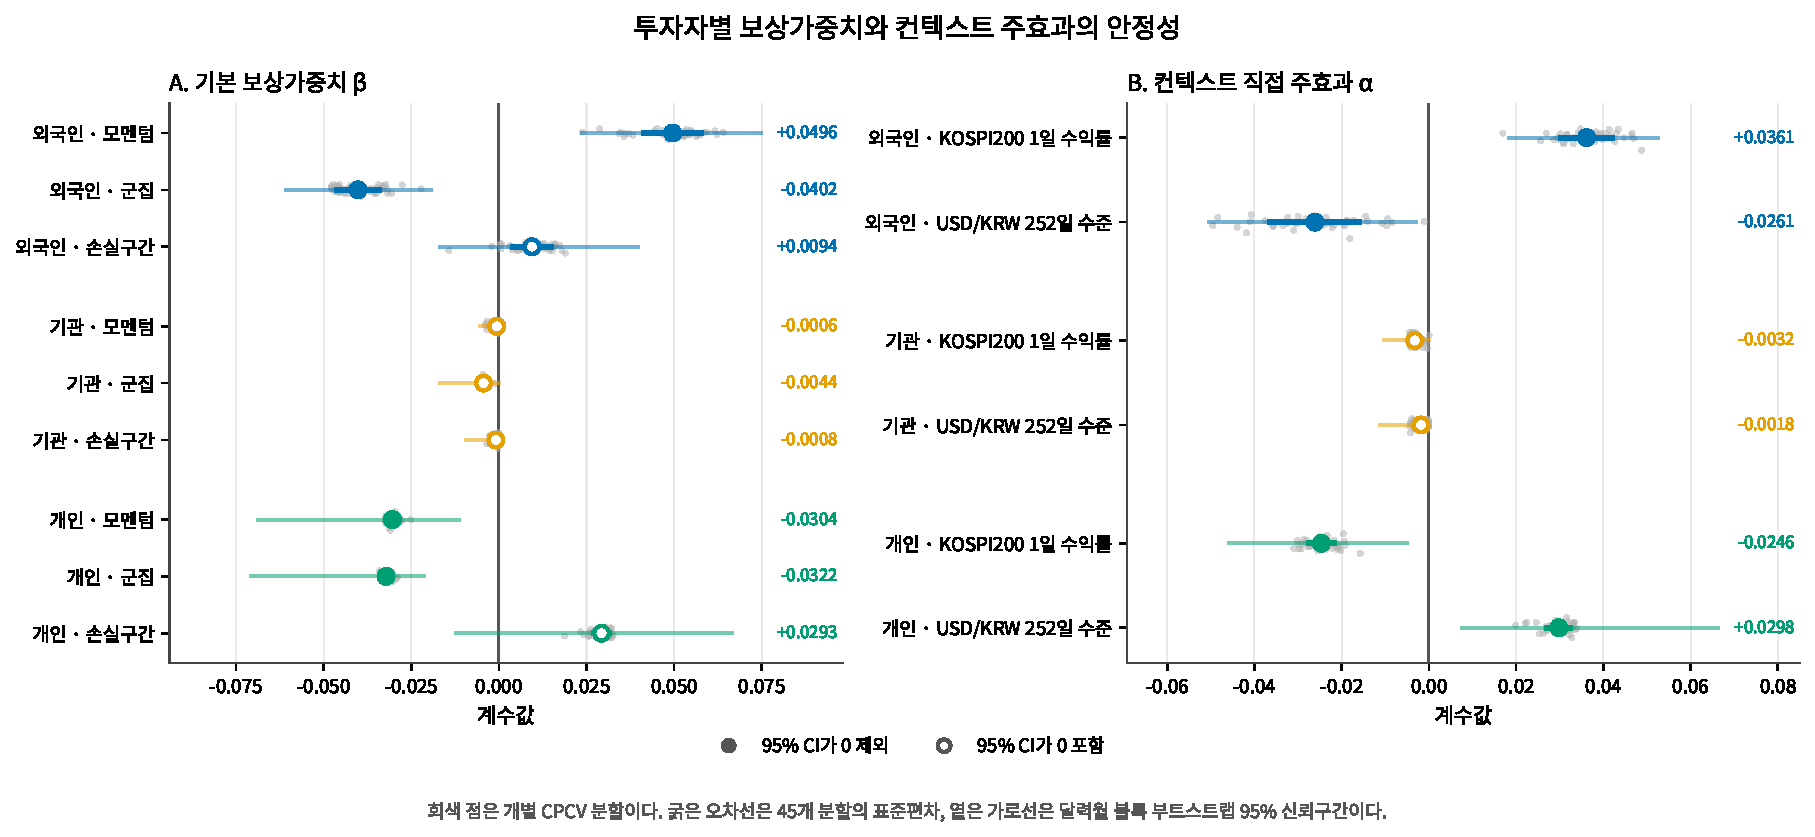
\includegraphics[width=\textwidth]{figures/fig_beta_alpha_forest.pdf}
  \caption{복원된 기본 보상가중치 $\beta$(A)와 컨텍스트 주효과 $\alpha$(B)의 안정성.
  회색 점은 45개 개별 CPCV 분할, 굵은 오차선은 분할 간 표준편차, 옅은 가로선은 달력월
  블록 부트스트랩 95\% 신뢰구간이다. 속이 빈 표식은 신뢰구간이 0을 포함하는 항이다.}
  \Description{두 패널의 forest plot. 패널 A는 세 유형의 모멘텀, 시차 교차연관,
  손실구간 계수를, 패널 B는 KOSPI200과 환율 주효과를 보인다. 외국인 모멘텀은 양,
  개인 모멘텀은 음이며 기관의 모든 표식은 속이 비어 있다.}
  \label{fig:forest}
\end{figure*}

\begin{table*}[t]
  \caption{(F1)--(F3) 주 사양과 지연 자기행동을 포함한 승격 사양의 계수 대조.
  값은 정확해 CPCV 45개 분할 평균, 괄호는 부호 일관성, CI는 달력월 블록 부트스트랩
  1{,}000회의 95\% 신뢰구간이며 $^{*}$는 0을 제외함을 뜻한다. 주 표(표~\ref{tab:performance},
  그림~\ref{fig:forest})의 Adam 수치는 변경하지 않았다.}
  \label{tab:spec34}
  \small
  \centering
  \begin{tabular}{@{}llcccc>{\raggedright\arraybackslash}p{0.14\textwidth}@{}}
    \toprule
    유형 & 항 & (F1)--(F3) 평균 & CI & 승격 사양 평균 & CI & 판정 \\
    \midrule
    \inputrows{sections/generated/tab3_body.tex}
    \bottomrule
  \end{tabular}
\end{table*}

\textbf{청산 제약이 정하는 해석의 경계.} 유형 간 계수를 비교하기 전에, 시장 청산이
기계적으로 만들 수 있는 것부터 정량화한다. 본 표본에서 외국인 순매수 1원은 평균적으로
개인 $-0.92$원, 기관 $-0.06$원, 기타 $-0.02$원으로 흡수되고, 유형별 총거래금액
비율은 $\mathbb{E}[W_{f}/W_{r}]=1.21\text{--}1.42$다. 따라서 외국인이 표준화 특징
$x$에 $\beta_f$만큼 반응하면, 개인이 아무 선호가 없어도 개인 계수에는
$\beta_{r}^{ind}\approx-0.92\times\beta_f\times(1.21\text{--}1.42)$의 성분이
유도된다(유도 과정과 가정은 부록~\ref{app:derivation}). 관측된 외국인 계수를 대입한
유도 성분은 \textbf{관측된 개인 계수를 전 항목에서 초과하거나 근사한다(관측의
84--214\%; 부록 표~\ref{tab:A2})}. 외국인만 선호를 갖는 합성 세계 1{,}000회의 전체
파이프라인 추정도 같은 결론을 준다. 개인이 물려받는 $\beta^{mom}$ 분포는
$[-0.101,-0.015]$로 관측치를 내부에 품으며, 이 세계는 동시점 상관 $-0.74$(관측
$-0.77$)와 기관의 null까지 재현한다. 반대로 선호가 전혀 없는 합성 세계에서
$\beta^{mom}$과 $\alpha$의 95\% 대역은 $\pm0.04$ 이내이므로 외국인의 $+0.0496$은 그
대역 밖(약 4.3 표준편차)에 있다. 이 두 사실이 본 절의 서술 규칙을 정한다. 유형별
계수 중 기계 대역을 초과하는 것만 선호로 읽고, 유도 범위 안의 것은 집계 수급의
구조로 읽는다.

\textbf{모멘텀 축의 거울상.} 외국인의 모멘텀 가중치는 $+0.0496$으로 45개 분할
전부에서 양수, 개인은 $-0.0304$로 전부에서 음수이며 두 부트스트랩 신뢰구간은 서로
겹치지 않고 각각 0을 제외한다(그림~\ref{fig:forest}A). 이 대비는 지연 자기행동을
통제한 승격 사양에서도 그대로 살아남는다(외국인 $+0.0331$, CI $[+0.0126,+0.0522]$;
개인 $-0.0261$, CI $[-0.0519,-0.0007]$; 표~\ref{tab:spec34}). walk-forward 10개
창에서 두 경로가 한 번도 교차하지 않으며(그림~\ref{fig:wf4}A), 벌점 종류와
$\lambda$ 통일에도 불변이다(부록 표~\ref{tab:A3}). 해석은 비대칭적이다. 외국인의
양수는 무선호 합성 대역 밖이고 자기상관ㆍ청산 통제를 모두 통과하므로 추세추종
선호로 읽으며, 이는 외국인 추세거래
문헌~\cite{grinblatt2000investment,choe1999foreign}과 부합한다. 개인의 음수는
부호와 안정성이 같은 검증을 통과하지만 크기가 청산 유도 범위 안에 있으므로,
독립적 역추세 선호의 증거로 읽지 않고 \emph{외국인의 추세거래가 청산 제약을 통해
개인 집계 수급에 남기는 반대 부호}까지만 주장한다. 개인 고유의 역추세 성향이 있는지는
이 자료의 집계 수준에서 식별되지 않는다.

\textbf{컨텍스트 주효과: 서술적 결과로 격하.} 주 사양의 $\alpha$ 네 계수(외국인
$+0.0361$/$-0.0261$, 개인 $-0.0246$/$+0.0298$)는 45개 분할 전부에서 부호가 유지되고
신뢰구간이 0을 제외한다(그림~\ref{fig:forest}B). 그러나 두 가지 이유로 본 연구는
이를 선호의 거울상이 아니라 ``관측된 집계 수급의 음의 교차 연관''이라는 서술적
결과로 제한한다. 첫째, 유도 성분이 관측을 초과한다(부록 표~\ref{tab:A2}). 둘째,
$\alpha^{KOSPI}$는 지연 자기행동을 통제하면 개인에서 $+0.0274$(45개 분할 전부 양수,
CI $[+0.0039,+0.0532]$)로 \textbf{부호가 반전}되고 외국인에서 $+0.0128$로 축소되어
CI가 0을 포함한다(표~\ref{tab:spec34}). 즉 주 사양의 개인 음수 $\alpha^{KOSPI}$는
개인 수급의 자기상관을 $\alpha$가 대신 흡수한 결과였다. $\alpha^{FX}$의 대비(외국인
$-0.0217$, 개인 $+0.0303$)만이 통제 후에도 CI를 유지하는 컨텍스트 결과다.

\textbf{유형 간 시차 교차연관.} 이 계수는 세 유형 모두 45개 분할 전부에서 음수이고
외국인($-0.0402$)과 개인($-0.0322$)은 신뢰구간도 0을 제외한다. 그러나 선호가 전혀
없는 합성 수급에서도 이 계수는 외국인 $[-0.057,-0.018]$, 개인 $[-0.085,-0.011]$로
음수가 되며 관측치는 두 대역의 내부에 있다(부록 표~\ref{tab:A2b}). 따라서 음의 시차
교차연관은 행동적 해석 없이 청산 제약과 자기상관만으로 발생 가능한 크기이며, 본
연구는 이를 서술적 결과로만 보고한다.

\textbf{손실구간.} 개인의 손실구간 가중치는 $+0.0293$으로 45개 분할 전부에서
양수이며 처분효과 문헌~\cite{shefrin1985disposition,odean1998investors}의 기준가격
의존성과 정합한다. 그러나 그림~\ref{fig:forest}A에서 보듯 세 유형 모두 신뢰구간이
0을 포함한다. 개인의 구간은 $[-0.0122,+0.0665]$로, 45개 분할에서 부호가 100\%
일관됨에도 월 블록 재표집에서는 5.5\%가 부호를 뒤집으며, 지연 자기행동을 통제하면
$+0.0115$(77.8\%)로 더 약해진다(표~\ref{tab:spec34}). 이는 CPCV 분할이 관측을
공유하기 때문에 부호 일관성이 불확실성을 과소평가한다는 \S\ref{sec:protocol}의
경고가 실제로 작동한 사례다. 따라서 처분효과와 정합하는 부호를 관측했다고 보고하되
통계적으로 확립된 결과로 주장하지 않는다.

\textbf{상호작용.} $B$ 12개는 동시에 검토한 탐색적 항목이다. 정확해 기준으로 45개
분할 부호가 유지되고 부트스트랩을 통과하는 항은 외국인
모멘텀$\times$KOSPI200($-0.0141$)과 개인 손실구간$\times$환율($-0.0408$)이다. Adam
해에서 100\% 일관으로 보였던 개인 모멘텀$\times$환율($+0.0144$)은 정확해에서
$-0.0106$(음수 91.1\%)으로 뒤집히므로 목록에서 제외한다(부록 표~\ref{tab:A1}).

\subsection{안정성}
\label{sec:stability}

\begin{figure*}[t]
  \centering
  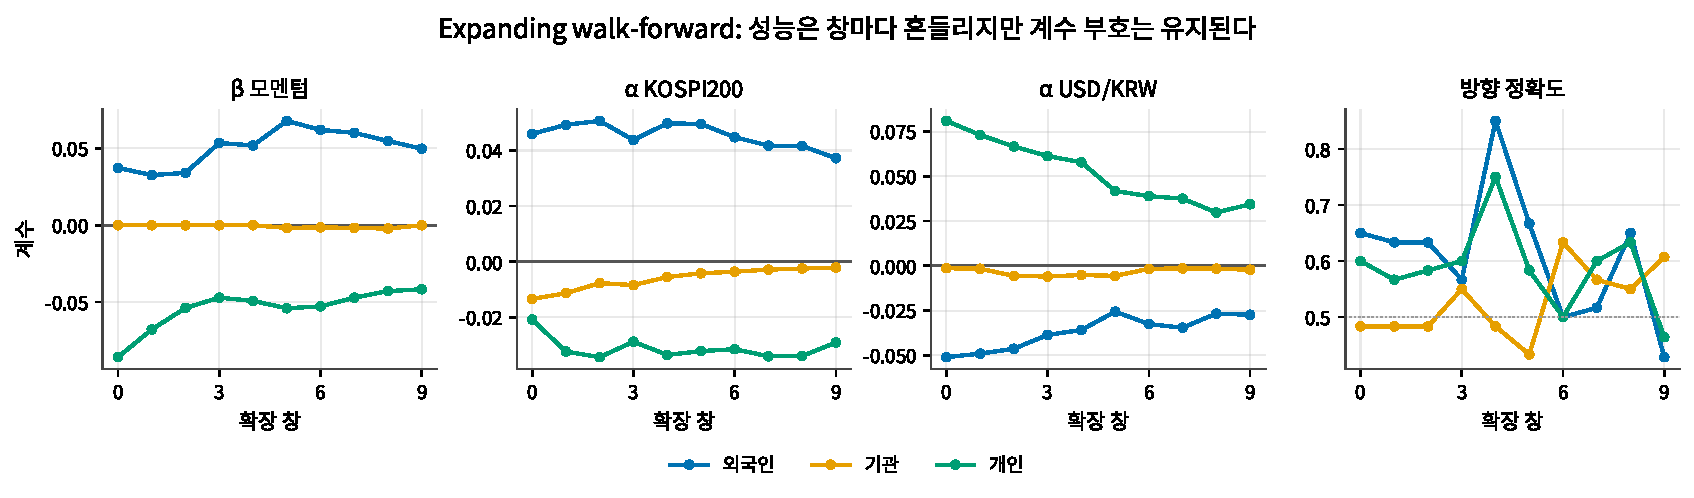
\includegraphics[width=\textwidth]{figures/fig_walk_forward.pdf}
  \caption{Expanding walk-forward 10개 창의 계수 경로와 방향 정확도((F1)--(F3) 주
  사양). 성능은 창마다 흔들리지만 계수 부호는 유지되며, 외국인과 개인의 모멘텀
  경로는 한 번도 교차하지 않는다.}
  \Description{확장 창 번호를 가로축으로 하여 세 유형의 모멘텀 계수, 두 컨텍스트
  주효과, 방향 정확도를 그린 네 개의 선그래프.}
  \label{fig:walkforward}
\end{figure*}

\begin{figure*}[t]
  \centering
  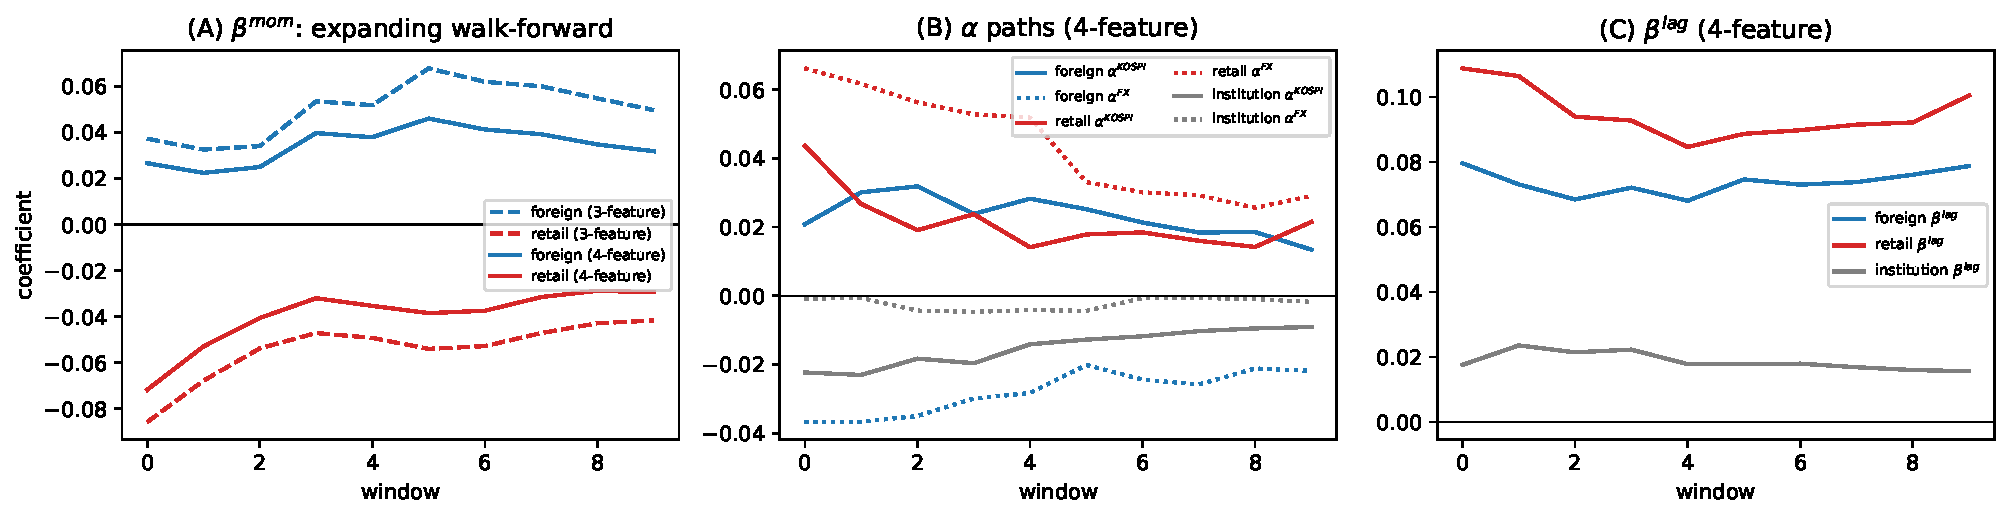
\includegraphics[width=\textwidth]{figures/fig3ext_walk_forward_4feature.pdf}
  \caption{승격 사양의 walk-forward 계수 경로(그림~\ref{fig:walkforward}의 확장).
  (A) $\beta^{mom}$: 점선은 (F1)--(F3), 실선은 승격 사양이며 두 유형의 경로가 어느
  사양에서도 교차하지 않는다. (B) 승격 사양의 $\alpha$ 경로: 개인 $\alpha^{KOSPI}$가
  10개 창 전부에서 양수다. (C) 지연 자기행동 계수 $\beta^{lag}$.}
  \Description{세 패널의 선그래프. 왼쪽 패널은 외국인과 개인의 모멘텀 계수 경로를
  3특징과 4특징 사양에 대해 각각 실선과 점선으로 보이고, 가운데 패널은 세 유형의
  KOSPI200 및 환율 주효과 경로를, 오른쪽 패널은 세 유형의 지연 자기행동 계수를
  보인다.}
  \label{fig:wf4}
\end{figure*}

\textbf{(V2)} 부트스트랩 결과는 셋으로 갈린다. 모멘텀 거울상과 컨텍스트 거울상을
이루는 8개 항이 모두 0을 제외하고, 손실구간은 통과하지 못하며, 기관은 어떤 항도
0을 제외하지 못한다(그림~\ref{fig:forest}의 속 빈 표식).

\textbf{(V3)} 그림~\ref{fig:walkforward}에서 성능은 크게 흔들린다. 외국인 방향
정확도는 0.43--0.85를 오가며 평균 $0.610\pm0.116$, 상관은 $0.131\pm0.162$로 CPCV의
0.278에서 절반 이하다. CPCV는 시험 폴드를 학습 폴드보다 앞세울 수 있는 반면
walk-forward는 그렇지 않으므로, 본 연구는 이 저하를 시간 구조에서 오는 일반화
한계로 그대로 보고한다. 반면 계수 경로는 흔들리지 않는다. 외국인 모멘텀은 10개 창
전부 양수, 개인은 전부 음수이며 두 경로가 한 번도 교차하지 않고, 두 컨텍스트
주효과에서도 같은 거울상이 유지된다. 기관의 경로는 0선에 붙어 있다.

\textbf{(V4)} 외국인과 개인의 계수는 $L_1$, $L_2$, 무벌점에서 소수점 넷째 자리까지
일치하므로 거울상은 벌점의 산물이 아니다. 반면 기관의 계수만 벌점에 따라
이동한다(시차 교차연관 $-0.0076\rightarrow-0.0124$, 손실구간
$-0.0000\rightarrow-0.0018$).

\textbf{승격 사양의 검증.} 지연 자기행동을 포함한 사양에도 V1--V4를 동일하게
적용했다(표~\ref{tab:spec34}, 그림~\ref{fig:wf4}). 모멘텀 대비와 $\alpha^{FX}$
대비는 네 검증을 모두 통과하고(walk-forward 10/10 창 부호 유지, 경로 비교차),
$\alpha^{KOSPI}$는 개인에서 10개 창 전부 양수로 반전되며, 손실구간은 약화된다.
외국인ㆍ개인 계수가 $L_1$/$L_2$/무벌점에서 소수 넷째 자리까지 일치하고 기관만
이동하는 패턴도 주 사양과 동일하다. 지연 자기행동을 컨텍스트와 상호작용시킨 확장
사양에서는 해당 상호작용 6개 항 전부의 CI가 0을 포함하며 다른 항의 변화는 0.0015
이내이므로, 본문은 파라미터 절약을 위해 $\beta$ㆍ$\alpha$만 확장한 사양을 보고한다.

\subsection{기관: 수렴된 null}
\label{sec:null}

기관 수급에 대해 SPR-IRL은 일별 빈도에서 안정적으로 식별되는 선호를 찾지 못했고,
본 연구는 이를 은폐하지 않고 결과로 보고한다. 근거는 다섯이다. (i) 예측 계열이 0선에
퇴화한다(그림~\ref{fig:prediction}). (ii) 시차 교차연관을 제외한 계수의 크기가 다른
유형보다 한 자릿수 이상 작다---현행 $\lambda$에서 $-0.0006$ㆍ$-0.0008$(약 $1/40$),
$\lambda$를 0으로 통일해도 $-0.0029$ㆍ$-0.0018$(약 $1/15$--$1/20$; 부록
표~\ref{tab:A3}). (iii) 부트스트랩에서 0을 제외하는 항이 없다(그림~\ref{fig:forest}).
(iv) 계수가 벌점 선택에 좌우된다. (v) walk-forward 10개 창에서 모멘텀 부호 일관성이
40\%, 손실구간이 0\%다.

\textbf{이 null은 최적화 실패가 아니다.} 명제~\ref{prop:lasso}에 따라 기관의 학습
인덱스에서 제약 문제~\eqref{eq:closs}은 볼록이고 그 해가 유일하다. 도달한 해와 동일
목적함수의 폐쇄형 최적해를 비교하면 기관의 목적함수 상대 격차는 평균 0.17\%, 최대
0.48\%에 불과하다(외국인 0.21\%, 개인 0.92\%). 세 유형 모두 도달 가능한 최적해에
근접했고, 기관에서만 그 최적해의 계수가 0 근방이다. 데이터가 기관에 대해 결정하는
선호가 없는 것이지 최적화가 찾지 못한 것이 아니다. 이 벌점 의존성은 계수 수준에서도
확인된다. 기관의 모멘텀ㆍ손실구간 좌표에서 목적함수 상대 격차 0.2\% 이내의 두
해---보고된 확률적 해와 폐쇄형 해---가 각각 $-0.0006$ㆍ$-0.0008$과 정확히 0(45개
분할 중 36개ㆍ44개)을 주므로, 이 좌표들에서 목적함수는 사실상 평평하며 0이 아닌
잔여값과 그로부터 계산된 부호 일관성(71\%ㆍ80\%)은 신호가 아니라 최적화
잔여물이다(부록 표~\ref{tab:A1}).

경제적으로 이 null은 투자자 분류에 대한 발견으로 읽어야 한다. ``기관''은 연기금,
투신, 보험, 사모, 금융투자를 합산한 범주다. 이 범주의 일평균 총거래금액은 958억
원으로 세 유형 중 가장 크지만 순매수 강도의 표준편차는 0.125로 가장 작다---큰
총거래가 반대 방향으로 상쇄되고 있다는 직접적 흔적이다. 상이한 목적함수를 가진 세부
주체들의 수급을 합산하면 일별 빈도에서 식별되는 공통 선호가 남지 않는다는 것이 본
결과의 내용이며, 세부 주체 분해는 \S\ref{sec:future}의 검정 가능한 가설로 남긴다.

다만 이 null은 특징 공간에 한정된다. 지연 자기행동을 통제한 승격 사양에서 기관은
$\alpha^{KOSPI}=-0.0113$(45개 분할 전부 음수, CI $[-0.0209,-0.0031]$)과 자기지연
$+0.0175$를 보이므로(표~\ref{tab:spec34}), ``어떤 항도 부트스트랩을 통과하지
못한다''는 서술은 (F1)--(F3) 주 사양에 한정해 유지한다.

\subsection{구성 타당성 점검}
\label{sec:construct}

\begin{table}[t]
  \caption{사전 부호 기대와 복원 결과}
  \label{tab:construct}
  \small
  \begin{tabular}{@{}>{\raggedright\arraybackslash}p{0.30\columnwidth}
                  >{\raggedright\arraybackslash}p{0.13\columnwidth}
                  >{\raggedright\arraybackslash}p{0.26\columnwidth}
                  >{\raggedright\arraybackslash}p{0.16\columnwidth}@{}}
    \toprule
    규칙성 & 사전 기대 & 복원 결과 & 판정 \\
    \midrule
    외국인 추세거래~\cite{grinblatt2000investment,choe1999foreign}
      & $\beta^{mom}\!>\!0$ & $+0.0496$ (100\%, CI 0 제외) & 부합 \\
    개인 역추세~\cite{grinblatt2000investment,kaniel2008individual}
      & $\beta^{mom}\!<\!0$ & $-0.0304$ (100\%, CI 0 제외) & 부합, 단 청산 유도 범위 내 \\
    처분효과~\cite{shefrin1985disposition,odean1998investors}
      & $\beta^{uw}\!>\!0$ & $+0.0293$ (100\%, CI 0 포함) & 부분 부합 \\
    기관 시차 교차연관 (참조:~\cite{lakonishok1992impact})
      & $\beta^{herd}\!>\!0$ & $-0.0044$ (100\%, CI 0 포함) & 측정 대상 상이 \\
    \bottomrule
  \end{tabular}
\end{table}

표~\ref{tab:construct}이 대조 결과다. 동일한 특징과 모형 형태를 부여하고 파라미터만
분리 학습했음에도 복원된 부호가 독립적으로 확립된 규칙성과 부합하고 두 유형이
모멘텀에서 정반대로 갈린다는 점이 구성 타당성의 증거다. 마지막 행은 측정 대상이
다르기 때문에 불일치로 보인다. Lakonishok 외~\cite{lakonishok1992impact}는 기관
\emph{내부}의 군집을, 식~\eqref{eq:herd}은 기관이 \emph{다른 두 유형}과 같은 방향으로
움직이는지를 측정하므로 본 결과는 해당 문헌의 반증이 아니다. 나아가
\S\ref{sec:beta}의 합성 실험은 음의 시차 교차연관이 선호 없이 청산 제약만으로
발생함을 보이므로, 이 항목은 구성 타당성 대조가 아니라 식별 경계의 예시로 읽는 것이
옳다.

%  의존:  sections/generated/*.tex (scripts/revision_20260727_make_tex_tables.py 산출)
% =====================================================================

\section{방법: SPR-IRL}
\label{sec:method}

본 절은 대칭 선호복원(Symmetric Preference Recovery, 이하 SPR-IRL) 절차를
정의한다. SPR-IRL은 모형 하나가 아니라 (i) 공유 특징 위의 대칭 추정, (ii) 표본외
안정성 평가, (iii) 사전 부호 기대와의 대조로 이루어진 절차다.

\subsection{연속 행동과 대칭 추정}
\label{sec:setup}

투자자 유형을 $\mathcal{I}=\{\text{외국인},\text{기관},\text{개인}\}$으로 둔다.
유형 $i$의 $t$일 총매수ㆍ총매도금액을 $V^{buy}_{i,t}$, $V^{sell}_{i,t}$라 하면
행동을
\begin{equation}
u_{i,t}=\frac{V^{buy}_{i,t}-V^{sell}_{i,t}}
             {V^{buy}_{i,t}+V^{sell}_{i,t}}\in[-1,1]
\label{eq:action}
\end{equation}
로 정의한다. 분모가 시장 전체가 아니라 해당 유형의 총거래금액이므로 $u_{i,t}$는
유형별 거래 규모에 영향받지 않는 공통 척도가 되며, 이진 라벨과 달리 강도 정보를
보존한다.

세 유형은 동일한 상태 특징 $x_{i,t}\in\mathbb{R}^{3}$, 동일한 컨텍스트
$C_t\in\mathbb{R}^{2}$, 동일한 모형 형태를 부여받고 파라미터
$\theta_i=(\beta_i,B_i,\alpha_i)$만 각자의 데이터로 분리 학습한다. 유형별로 다른
특징을 미리 배정하지 않으므로, 결과의 유형 간 차이는 설계가 아니라 데이터에서
학습된 것이며 이것이 계수의 직접 비교를 정당화한다.

학습 표본은 $(x_{i,t},C_t,a_{i,t+1})$, $a_{i,t+1}=u_{i,t+1}$이다. $t$일 상태가
$t+1$일 행동을 설명하므로 미래 거래는 특징에 들어가지 않는다.

\subsection{보상 특징과 시장 컨텍스트}
\label{sec:features}

세 특징과 두 컨텍스트는 모두 각 분할의 학습 인덱스에서만 표준화하므로, 이후 계수는
1표준편차 변화의 효과로 읽는다.

\textbf{(F1) 중기 모멘텀} $x^{mom}_{t}=\log(P_t/P_{t-20})$. 20거래일은 해석을 위한
사전 지정값이며 자료에서 최적화하지 않았다. 양수는 추세추종, 음수는 역추세를 뜻하고
부호 기대는 유형별 모멘텀 거래 문헌~\cite{grinblatt2000investment,choe1999foreign}에서
온다. 이 창과 (F3)의 망각계수 $\rho=0.98$은 사전 지정값이며,
$\rho\in\{0.95,0.98,0.99\}\times$창$\in\{10,20,60\}$의 아홉 조합 전부에서
\S\ref{sec:beta}의 모멘텀 부호 대비와 개인 손실구간 부호가 유지된다(부록
표~\ref{tab:A4}).

\textbf{(F2) 유형 간 시차 교차연관} 유형 $i$를 제외한 두 유형의 전일 행동 횡단면
평균
\begin{equation}
x^{herd}_{i,t}=\tfrac{1}{2}\left(u_{j,t-1}+u_{k,t-1}\right),\qquad j,k\neq i.
\label{eq:herd}
\end{equation}
1거래일 지연은 정보 제약이 아니라, 동일 거래일 유형 간 수급의 회계적 상쇄를 예측
변수에서 배제하기 위한 설계 선택이다(\S\ref{sec:beta}). 부호 기대는 기관 군집행동
문헌~\cite{lakonishok1992impact}을 참조하되, 해당 문헌은 기관 \emph{내부}의 군집을,
식~\eqref{eq:herd}은 \emph{유형 간} 시차 관계를 측정하므로 이 특징의 계수는
군집행동의 직접 검정이 아니다(\S\ref{sec:construct}).

\textbf{(F3) 평균단가 대비 손실구간} 평균단가 대용치 $\bar P_{i,t}$와 당일 총거래
VWAP $P^{vwap}_{i,t}$로
\begin{equation}
x^{uw}_{i,t}=\max\!\left(
\frac{\bar P_{i,t}-P^{vwap}_{i,t}}{\bar P_{i,t}},\,0\right).
\label{eq:underwater}
\end{equation}
0에서 절단하므로 이 변수는 준거점 의존적 설계다. 평균단가는 총매수ㆍ총매도 수량과
금액으로 유효 보유량을 재귀 갱신해 구하되 전일 보유량에 망각계수 $\rho=0.98$을
곱한다(반감기 약 34거래일). 부호 기대는 처분효과
문헌~\cite{shefrin1985disposition,odean1998investors}에서 온다. 다만 이 대용치는
집계 거래로 만든 근사치이므로 $x^{uw}$의 계수를 처분효과의 직접 검정으로 읽을 수
없다.

\textbf{컨텍스트}는 KOSPI200 1일 수익률 $r_t$와 원/달러 환율 수준
$z_t=(\log e_t-\mu_{t-1,252})/\sigma_{t-1,252}$이다. 평균과 표준편차는 $t-1$까지의
252거래일만 쓴다. 삼성전자의 KOSPI200 비중 때문에 종목 모멘텀과 시장수익률이
겹치며 특징--컨텍스트 상관은 $-0.29$에서 $0.22$ 범위다. 따라서 개별 계수는 다른
항이 통제된 조건부 연관이다.

\subsection{근시안적 보상과 제약 Lasso로의 환원}
\label{sec:model}

유형 $i$의 행동점수를
\begin{equation}
q_{i,t}=(\beta_i+B_iC_t)^{\top}x_{i,t}+\alpha_i^{\top}C_t
\label{eq:score}
\end{equation}
로 둔다. $\alpha$는 종목 특징이 평균일 때도 행동 수준을 옮기는 수준효과, $B$는
컨텍스트에 따라 특징 민감도가 달라지는 기울기 효과다. 상호작용을 넣으면서 하위차수
항 $C_t$를 빼는 것은 표준적 사양 오류이므로 $\alpha$의 포함은 자료로 정당화할
대상이 아니다. 연속 행동에 대한 단기 보상을
$R_i=q_{i,t}a-\tfrac{\kappa}{2}a^{2}$로 두면 최적 정책은
\begin{equation}
a^{*}_{i,t+1}=\mathrm{clip}(q_{i,t}/\kappa,-1,1)
\label{eq:policy}
\end{equation}
이다. 이차항이 없으면 해가 거의 항상 $\pm1$이 되어 행동 강도를 재현할 수 없다.
$\kappa$는 식별을 위해 1로 고정하며, 이는 보상과 계수의 단위를 고정하는 정규화이지
곡률이 경험적으로 1이라는 주장이 아니다. 학습목적은
\begin{equation}
\min_{\theta_i}\ \frac{1}{|\mathcal{D}_i|}
\sum_{t\in\mathcal{D}_i}\!\bigl(a^{*}_{i,t+1}-a_{i,t+1}\bigr)^{2}
+\lambda_i\lVert\theta_i\rVert_1
\label{eq:loss}
\end{equation}
이다. 여기서
\[
\begin{aligned}
z_{i,t}&=[\,x_{i,t};\ \mathrm{vec}(x_{i,t}C_t^{\top});\ C_t\,]\in\mathbb{R}^{11},\\
\theta_i&=[\,\beta_i;\ \mathrm{vec}(B_i);\ \alpha_i\,]
\end{aligned}
\]
로 두면 $q_{i,t}=\theta_i^{\top}z_{i,t}$이므로 식~\eqref{eq:loss}은 $z$ 위의 벌점 회귀
형태를 갖는다.

\textbf{그러나 식~\eqref{eq:loss}은 볼록이 아니다.} 예측값이 절단되기 때문이다.
한 관측의 손실을
$\ell(u)=(\mathrm{clip}(u)-a)^2$라 하자. $a=0$이면
$\ell(-2)=\ell(-1)=1$, $\ell(0)=0$이므로
$\ell(-1)$이 두 값의 평균 $0.5$를 넘어 $\ell$은 볼록이 아니다. 더구나 $\mathrm{clip}$은 상자
$[-1,1]^{n}$으로의 사영이고 관측 행동이 그 상자 안에 있으므로 모든 $\theta$에서
\[
\lVert\mathrm{clip}(Z\theta)-a\rVert\ \le\ \lVert Z\theta-a\rVert
\]
가 성립한다. 즉 포화는 오차를 줄일 수도 있으며(부록~\ref{app:convexity}의 최소 예),
어떤 해에서 $|q|<1$임을 확인하는 것만으로 포화영역에 더 좋은 해가 없다고 결론지을 수
없다.

따라서 본 논문은 추정량을 처음부터 제약 문제로 정의한다. 학습 인덱스
$\mathcal{D}_i$에 대해 $\mathcal{C}_i=\{\theta:\ |z_{i,t}^{\top}\theta|\le 1,\
\forall t\in\mathcal{D}_i\}$로 두고
\begin{equation}
\hat\theta_i=\operatorname*{arg\,min}_{\theta\in\mathcal{C}_i}\ \frac{1}{|\mathcal{D}_i|}
\sum_{t\in\mathcal{D}_i}\bigl(z_{i,t}^{\top}\theta-a_{i,t+1}\bigr)^{2}
+\lambda_i\lVert\theta\rVert_1 .
\label{eq:closs}
\end{equation}
이 제약은 계산상의 편의가 아니라 식별 제약이다. 포화영역에서는
$\theta\mapsto\mathrm{clip}(Z\theta)$가 단사가 아니어서---모든 관측이 포화된 $\theta$는
$c>1$배 해도 예측이 같다---파라미터가 식별되지 않으며, $\lambda=0$이면 그 영역의
최적해는 연속체를 이룬다. $\mathcal{C}_i$는 정책이 내부해인 영역, 곧 계수를 행동 강도의
1표준편차 효과로 읽을 수 있는 영역이다.

\begin{proposition}[제약 Lasso 환원과 유일성]
\label{prop:lasso}
(a) $\mathcal{C}_i$ 위에서 식~\eqref{eq:loss}과 식~\eqref{eq:closs}의 목적식은 동일하다.
(b) 무제약 Lasso 해 $\tilde\theta_i$가 $\mathcal{C}_i$에 속하면 $\tilde\theta_i$는
식~\eqref{eq:closs}의 전역해이며, $\mathcal{C}_i$의 \emph{내부}에 속하면 두 문제의 KKT
조건이 일치한다(제약 승수가 0). (c) 식~\eqref{eq:closs}은 볼록 다면체 위의 볼록 문제이고,
$\lambda_i=0$일 때 $\mathrm{rank}(Z_i)=p$이면, $\lambda_i>0$일 때 등상관 집합
$E=\{j:|\tfrac{2}{n}z_{j}^{\top}(a-Z\hat\theta)|=\lambda_i\}$에 대해
$\mathrm{rank}(Z_{i,E})=|E|$이면 그 해는 유일하다.
\end{proposition}

증명은 부록~\ref{app:convexity}에 있다. 본 표본에서 세 조건이 모두 성립한다. 45개
분할$\times$3유형 전부에서 학습 인덱스의 $\max_t|z_t^{\top}\hat\theta|$가 0.558을 넘지
않아 해는 $\mathcal{C}_i$의 내부에 있고, $\mathrm{rank}(Z)=11$(최악 조건수 6.86)이며,
$\lambda>0$인 두 유형에서 $\mathrm{rank}(Z_E)=|E|$다(부록 표~\ref{tab:F1}). 따라서
식~\eqref{eq:closs}의 해는 존재하고 유일하며 무제약 Lasso 해와 일치한다. 이 영역
안에서 SPR-IRL의 ``선호를 복원한다''와 ``수급을 회귀한다''는 수치적으로 구별되지
않으며, 문제가 볼록이므로 좌표하강 정확해로 직접 풀 수 있다. 본 개정에서 보고하는
모든 확장 사양은 이 정확해로 추정했다(\S\ref{sec:null}, 부록 표~\ref{tab:A1}).

무제약 문제~\eqref{eq:loss}의 전역 최적성은 이와 별개이며 본 논문은 그것을 주장하지
않는다. 다만 부록~\ref{app:convexity}는 두 가지를 보고한다. 첫째, $\hat\theta$보다 나은
목적값을 갖는 어떤 $\theta$도 학습 관측의 20.7\%(외국인)ㆍ4.2\%(기관)ㆍ40.2\%(개인)를
넘게 포화시킬 수 없다는 증명 가능한 경계. 둘째, 분할ㆍ유형당 939개, 합계 42{,}255개
시작점의 다중시작 탐색에서 더 나은 해가 하나도 발견되지 않았다는 사실이다.

이 일치는 결함이 아니라 근시안 가정의 귀결이다. 한 걸음만 내다보면 오늘의 행동이
내일 이후에 영향을 주지 않으므로, 무엇을 원하는가(보상)와 무엇을 하는가(정책)가
하나로 겹친다. 최대엔트로피 IRL~\cite{ziebart2008maximum}의
$\pi\propto\exp(R/\tau)$를 적용하면 $\pi$는 평균 $q$의 절단정규분포가 되어
점추정치가 위와 일치하므로, 이 환원은 특정 구현의 우연이 아니라 근시안ㆍ이차보상
설정 전반의 성질이다. 역강화학습 정식화의 가치는 확장 경로에 있다. 상태 동역학과
다기간 가치를 넣는 순간 보상은 정책과 갈라지고 회귀로는 도달할 수 없는 구조적
복원이 된다(\S\ref{sec:discussion}).

\subsection{검증 프로토콜}
\label{sec:protocol}

복원된 계수를 그대로 보고하지 않고 네 단계를 거친다. \textbf{(V1)} 10개 시간 폴드
중 2개를 시험으로 쓰는 조합형 정화 교차검증~\cite{lopez2018advances}으로
$\binom{10}{2}=45$개 분할을 만들고, 1일 purge와 5일 embargo를 적용하며 모든
표준화는 학습 인덱스에만 적합한다. 분할들이 관측을 공유하므로 부호 일관성은
$p$-값이 아니라 안정성 지표로만 해석한다. \textbf{(V2)} 그 한계를 보완하기 위해
표본을 달력월 블록으로 나누어 1{,}000회 복원추출하고 95\% 신뢰구간을 구한다. 월
블록은 일별 수급의 자기상관을 블록 안에 보존한다. \textbf{(V3)} CPCV는 시험 폴드가
학습 폴드보다 앞설 수 있으므로, 최초 400개 관측에서 시작해 5일 purge 후 다음
60거래일을 예측하고 학습 구간을 60거래일씩 넓히는 expanding walk-forward를 10개 창
수행한다. \textbf{(V4)} 결과가 $L_1$ 벌점의 산물이 아님을 보이기 위해 $L_2$ 및
무벌점으로 재추정해 부호를 비교한다.

지표는 MAE, RMSE, 방향 정확도($\mathrm{sign}(a^{*})=\mathrm{sign}(a)$의 비율),
예측--실제 상관, 포화 비율이다. 유형 간 행동 표준편차가 다르므로 오차의 절대값은
유형 간 비교에 쓰지 않는다. 자명한 참조로 전일 자기행동을 그대로 예측하는 지속성
규칙을 함께 보고한다.

% =====================================================================
\section{실험}
\label{sec:experiments}

\subsection{데이터}
\label{sec:data}

삼성전자(005930) 일별 자료에서 252일 환율 이력, 20일 모멘텀, 다음 날 행동을 모두
계산할 수 있는 최신 973행을 사용한다. 상태일은 2022-01-06--2025-12-29이다. 단일
종목은 표본의 한계가 아니라 종목 고정효과와 유동성 차이를 배제하고 유형 간 선호
이질성만 분리하기 위한 통제된 설정이다.

행동 평균은 세 유형 모두 0에 가깝지만 표준편차는 개인 0.334, 외국인 0.257, 기관
0.125로 다르고, 1차 자기상관은 각각 0.345, 0.401, 0.149다. 동일 거래일 유형 간
행동은 강한 음의 관계를 갖는다(외국인--개인 $-0.772$, 기관--개인 $-0.499$). 이 음의
동시점 구조가 유형 간 계수 해석에 부과하는 식별 경계는 \S\ref{sec:beta}에서
정량화한다. 세 유형 순매수 합계와 시장 전체의 차이(기타법인ㆍ기타외국인 등)는
일평균 144억 원, 거래대금의 1.3\%에 그친다.

학습 설정은 유형별로 외국인 75 epochs / batch 256 / lr 0.001 / $\lambda=0$, 기관
10 / 2048 / 0.0005 / 0.01, 개인 20 / 512 / 0.001 / 0.0003이며 seed 42, $\kappa=1$,
유형당 파라미터 11개($\beta$ 3, $B$ 6, $\alpha$ 2)다. 유형별 $\lambda$는 본
사양에서 중첩 교차검증으로 선택된 값이 아니라, 선행 이산행동 사양에서 CPCV 정확도
그리드 탐색으로 정해져 이월된 값이다. 따라서 $\lambda$ 비대칭이 결과를 만드는지
확인하기 위해 세 유형에 동일한 $\lambda\in\{0,0.0005,0.01\}$을 부여한 재추정을 부록
표~\ref{tab:A3}에 함께 보고하며, 거울상 부호는 모든 $\lambda$ 사양에서 유지된다.

\subsection{표본외 행동 재현}
\label{sec:oos}

\begin{figure}[t]
  \centering
  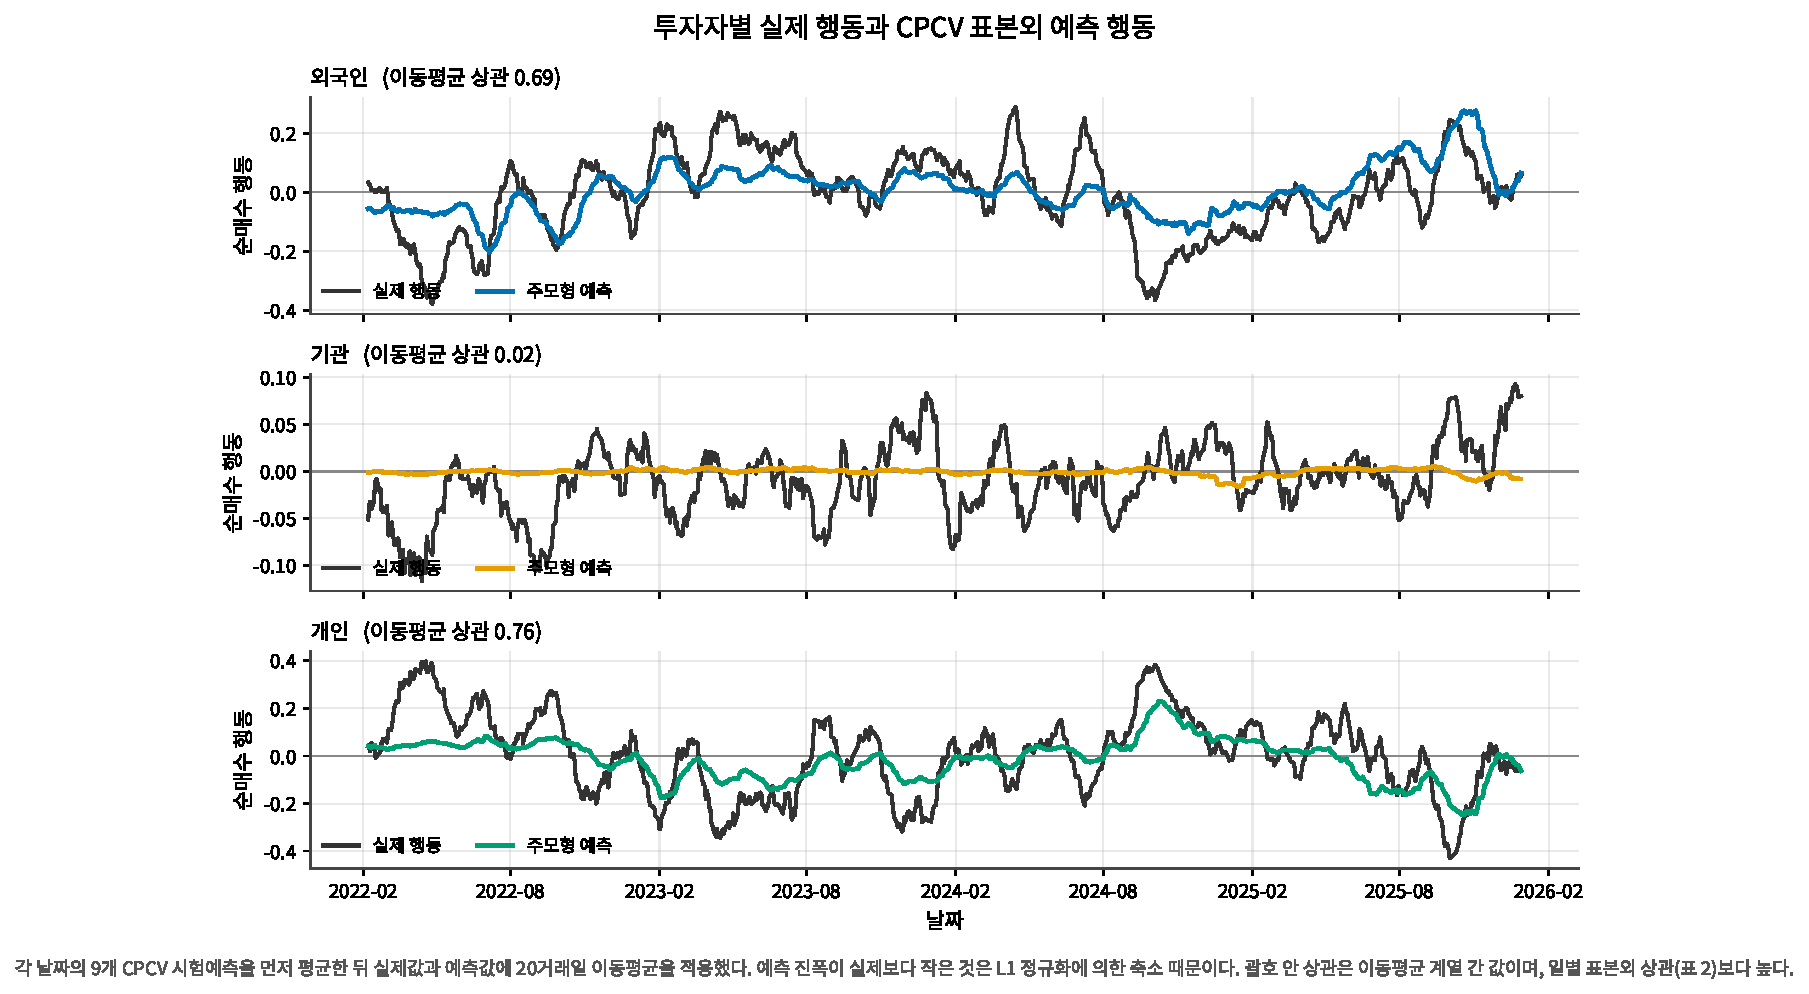
\includegraphics[width=\columnwidth]{figures/fig_actual_vs_prediction.pdf}
  \caption{실제 행동과 CPCV 표본외 예측(20거래일 이동평균). 각 날짜의 9개 시험예측을
  먼저 평균했다. 괄호 안은 평활 계열 간 상관으로,
  표~\ref{tab:performance}의 일별 상관과 직접 비교하지 않는다.}
  \Description{외국인, 기관, 개인의 실제 순매수와 모형 예측을 시간축에 겹쳐 그린
  세 개의 선그래프. 기관 패널에서 예측선이 0 근방에 평탄하게 놓여 있다.}
  \label{fig:prediction}
\end{figure}

\begin{table}[t]
  \caption{CPCV 표본외 성능(45개 분할 평균 $\pm$ 표준편차), 지속성 기준선, 그리고
  지연 자기행동을 포함한 승격 사양}
  \label{tab:performance}
  \small
  \centering
  \begin{tabular}{@{}lccc@{}}
    \toprule
    지표 & 외국인 & 기관 & 개인 \\
    \midrule
    \multicolumn{4}{@{}l}{\emph{SPR-IRL} (F1)--(F3), 주 사양}\\
    방향 정확도 & $0.636\pm0.039$ & $0.542\pm0.038$ & $0.608\pm0.044$ \\
    상관계수    & $0.278\pm0.110$ & $0.068\pm0.064$ & $0.245\pm0.118$ \\
    MAE         & $0.195\pm0.019$ & $0.094\pm0.008$ & $0.264\pm0.029$ \\
    MAE / 행동 SD & $0.759$ & $0.756$ & $0.791$ \\
    포화 비율   & $0.000$ & $0.000$ & $0.000$ \\
    \addlinespace
    \multicolumn{4}{@{}l}{\emph{지속성 기준선} ($a_{t+1}\!\leftarrow\!a_t$)}\\
    방향 정확도 & $0.642$ & $0.547$ & $0.616$ \\
    상관계수    & $0.359$ & $0.136$ & $0.311$ \\
    \addlinespace
    \multicolumn{4}{@{}l}{\emph{승격 사양} (F1)--(F3)$+u_{i,t}$, 정확해 (\S\ref{sec:beta})}\\
    \inputrows{sections/generated/tab1_rows.tex}
    \bottomrule
  \end{tabular}
\end{table}

그림~\ref{fig:prediction}에서 외국인과 개인의 예측 계열은 실제 계열의 국면 전환을
따라가지만(평활 상관 0.69, 0.76) 진폭은 작다. 이는 벌점의 산물이 아니라---외국인은
$\lambda=0$이다---설명력이 유한한 회귀의 조건부 기대가 갖는 일반적 성질이다. 표본외
$R^2$가 0.10--0.18인 예측치의 표준편차는 실제 행동 표준편차의 1/3 수준으로
축소된다. 기관의 예측 계열은 사실상 0선에 붙어 있다(0.02).

표~\ref{tab:performance}에서 세 가지가 드러난다. 첫째, 분할 간 산포가 커서 단일
분할의 수치로 유형을 비교할 수 없다. 둘째, 자명한 지속성 기준선이 방향 정확도와
상관계수에서 (F1)--(F3) 사양의 SPR-IRL을 앞선다. $a_t$는 $t$일 종가 이후 공개되므로
이는 정보상 이용 가능한 규칙이다. 셋째, 원인은 특징 집합의 설계에 있다. 행동의
자기상관이 $0.401/0.149/0.345$인데 (F1)--(F3)에는 자기 지연행동이 없다. 이 제한은
세 유형이 독립적으로 확립된 규칙성에 대응하는 특징만 공유하도록 한 선택이지 예측
성능을 위한 설계가 아니다. \textbf{지연 자기행동 $u_{i,t}$를 네 번째 특징으로 넣은
승격 사양은 세 유형 모두에서 지속성 기준선을 넘어서며(방향 정확도 $0.652/0.574/
0.629$, 표~\ref{tab:performance}), 이때 어떤 계수 부호가 살아남는지가
\S\ref{sec:beta}의 해석을 결정한다(표~\ref{tab:spec34}).} 즉 선호 복원과 수급
예측은 상이한 특징 집합을 요구하는 별개의 과제다.

모든 유형ㆍ모든 분할에서 학습 인덱스의 포화 비율이 0이므로 명제~\ref{prop:lasso}(b)의
전제가 성립하고, 제약 추정량~\eqref{eq:closs}은 무제약 Lasso와 일치한다. 승격 사양에서도
포화 비율은 45개 분할 전부 0이며 표본 전체에서 $|q|$의 최대값은 0.959다.

\subsection{복원된 구조: 모멘텀 축의 거울상과 그 식별 경계}
\label{sec:beta}

\begin{figure*}[t]
  \centering
  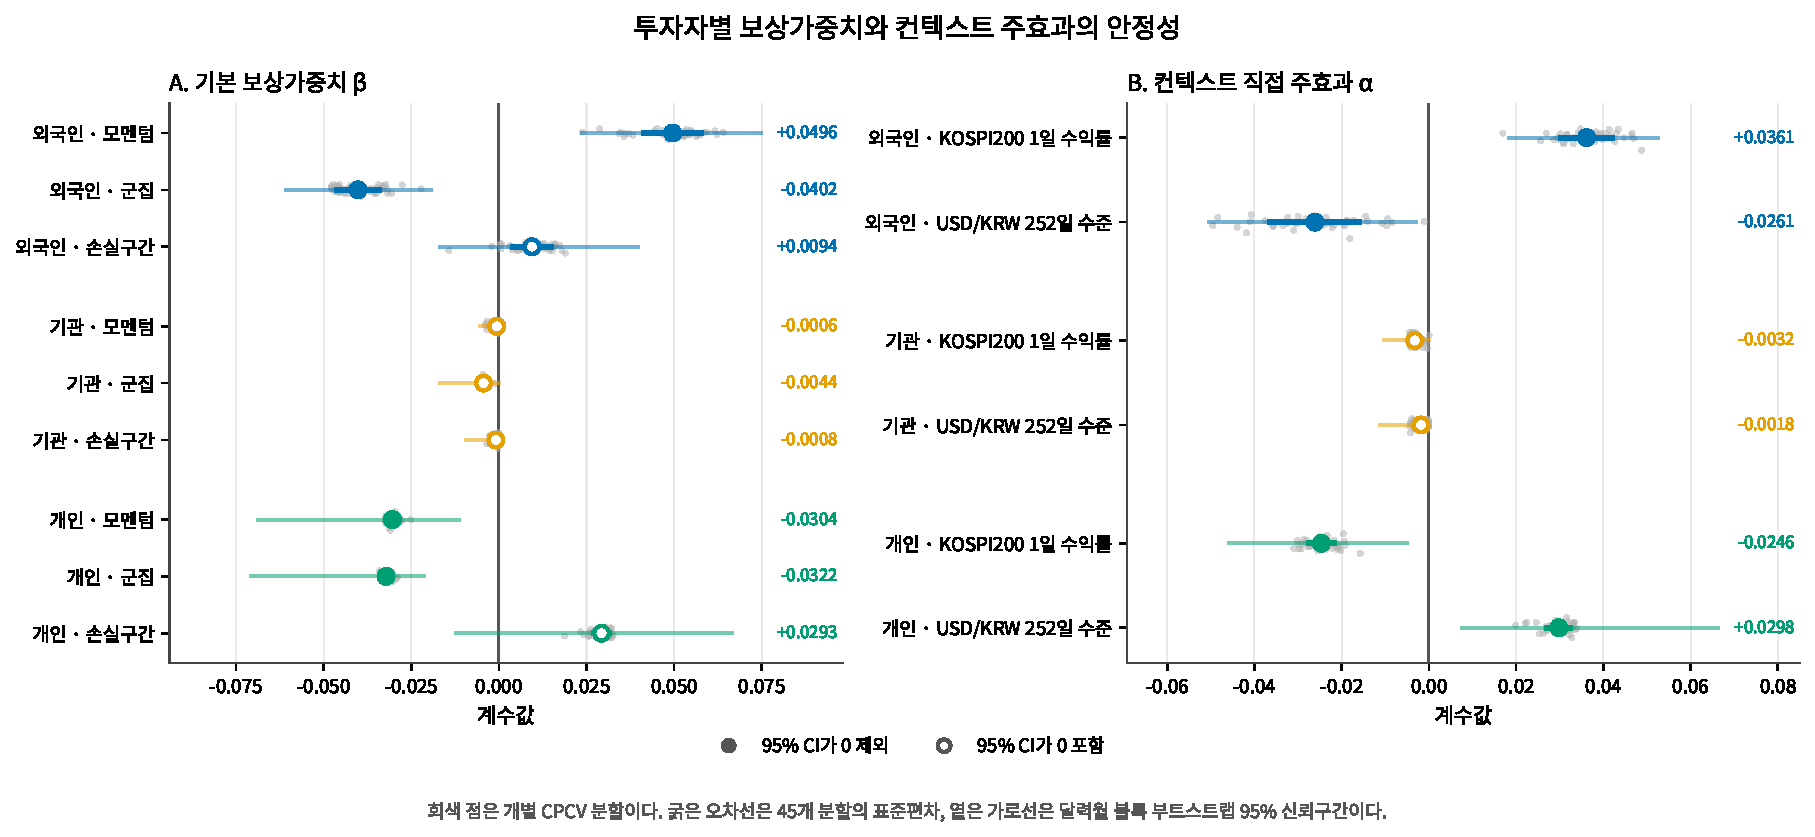
\includegraphics[width=\textwidth]{figures/fig_beta_alpha_forest.pdf}
  \caption{복원된 기본 보상가중치 $\beta$(A)와 컨텍스트 주효과 $\alpha$(B)의 안정성.
  회색 점은 45개 개별 CPCV 분할, 굵은 오차선은 분할 간 표준편차, 옅은 가로선은 달력월
  블록 부트스트랩 95\% 신뢰구간이다. 속이 빈 표식은 신뢰구간이 0을 포함하는 항이다.}
  \Description{두 패널의 forest plot. 패널 A는 세 유형의 모멘텀, 시차 교차연관,
  손실구간 계수를, 패널 B는 KOSPI200과 환율 주효과를 보인다. 외국인 모멘텀은 양,
  개인 모멘텀은 음이며 기관의 모든 표식은 속이 비어 있다.}
  \label{fig:forest}
\end{figure*}

\begin{table*}[t]
  \caption{(F1)--(F3) 주 사양과 지연 자기행동을 포함한 승격 사양의 계수 대조.
  값은 정확해 CPCV 45개 분할 평균, 괄호는 부호 일관성, CI는 달력월 블록 부트스트랩
  1{,}000회의 95\% 신뢰구간이며 $^{*}$는 0을 제외함을 뜻한다. 주 표(표~\ref{tab:performance},
  그림~\ref{fig:forest})의 Adam 수치는 변경하지 않았다.}
  \label{tab:spec34}
  \small
  \centering
  \begin{tabular}{@{}llcccc>{\raggedright\arraybackslash}p{0.14\textwidth}@{}}
    \toprule
    유형 & 항 & (F1)--(F3) 평균 & CI & 승격 사양 평균 & CI & 판정 \\
    \midrule
    \inputrows{sections/generated/tab3_body.tex}
    \bottomrule
  \end{tabular}
\end{table*}

\textbf{청산 제약이 정하는 해석의 경계.} 유형 간 계수를 비교하기 전에, 시장 청산이
기계적으로 만들 수 있는 것부터 정량화한다. 본 표본에서 외국인 순매수 1원은 평균적으로
개인 $-0.92$원, 기관 $-0.06$원, 기타 $-0.02$원으로 흡수되고, 유형별 총거래금액
비율은 $\mathbb{E}[W_{f}/W_{r}]=1.21\text{--}1.42$다. 따라서 외국인이 표준화 특징
$x$에 $\beta_f$만큼 반응하면, 개인이 아무 선호가 없어도 개인 계수에는
$\beta_{r}^{ind}\approx-0.92\times\beta_f\times(1.21\text{--}1.42)$의 성분이
유도된다(유도 과정과 가정은 부록~\ref{app:derivation}). 관측된 외국인 계수를 대입한
유도 성분은 \textbf{관측된 개인 계수를 전 항목에서 초과하거나 근사한다(관측의
84--214\%; 부록 표~\ref{tab:A2})}. 외국인만 선호를 갖는 합성 세계 1{,}000회의 전체
파이프라인 추정도 같은 결론을 준다. 개인이 물려받는 $\beta^{mom}$ 분포는
$[-0.101,-0.015]$로 관측치를 내부에 품으며, 이 세계는 동시점 상관 $-0.74$(관측
$-0.77$)와 기관의 null까지 재현한다. 반대로 선호가 전혀 없는 합성 세계에서
$\beta^{mom}$과 $\alpha$의 95\% 대역은 $\pm0.04$ 이내이므로 외국인의 $+0.0496$은 그
대역 밖(약 4.3 표준편차)에 있다. 이 두 사실이 본 절의 서술 규칙을 정한다. 유형별
계수 중 기계 대역을 초과하는 것만 선호로 읽고, 유도 범위 안의 것은 집계 수급의
구조로 읽는다.

\textbf{모멘텀 축의 거울상.} 외국인의 모멘텀 가중치는 $+0.0496$으로 45개 분할
전부에서 양수, 개인은 $-0.0304$로 전부에서 음수이며 두 부트스트랩 신뢰구간은 서로
겹치지 않고 각각 0을 제외한다(그림~\ref{fig:forest}A). 이 대비는 지연 자기행동을
통제한 승격 사양에서도 그대로 살아남는다(외국인 $+0.0331$, CI $[+0.0126,+0.0522]$;
개인 $-0.0261$, CI $[-0.0519,-0.0007]$; 표~\ref{tab:spec34}). walk-forward 10개
창에서 두 경로가 한 번도 교차하지 않으며(그림~\ref{fig:wf4}A), 벌점 종류와
$\lambda$ 통일에도 불변이다(부록 표~\ref{tab:A3}). 해석은 비대칭적이다. 외국인의
양수는 무선호 합성 대역 밖이고 자기상관ㆍ청산 통제를 모두 통과하므로 추세추종
선호로 읽으며, 이는 외국인 추세거래
문헌~\cite{grinblatt2000investment,choe1999foreign}과 부합한다. 개인의 음수는
부호와 안정성이 같은 검증을 통과하지만 크기가 청산 유도 범위 안에 있으므로,
독립적 역추세 선호의 증거로 읽지 않고 \emph{외국인의 추세거래가 청산 제약을 통해
개인 집계 수급에 남기는 반대 부호}까지만 주장한다. 개인 고유의 역추세 성향이 있는지는
이 자료의 집계 수준에서 식별되지 않는다.

\textbf{컨텍스트 주효과: 서술적 결과로 격하.} 주 사양의 $\alpha$ 네 계수(외국인
$+0.0361$/$-0.0261$, 개인 $-0.0246$/$+0.0298$)는 45개 분할 전부에서 부호가 유지되고
신뢰구간이 0을 제외한다(그림~\ref{fig:forest}B). 그러나 두 가지 이유로 본 연구는
이를 선호의 거울상이 아니라 ``관측된 집계 수급의 음의 교차 연관''이라는 서술적
결과로 제한한다. 첫째, 유도 성분이 관측을 초과한다(부록 표~\ref{tab:A2}). 둘째,
$\alpha^{KOSPI}$는 지연 자기행동을 통제하면 개인에서 $+0.0274$(45개 분할 전부 양수,
CI $[+0.0039,+0.0532]$)로 \textbf{부호가 반전}되고 외국인에서 $+0.0128$로 축소되어
CI가 0을 포함한다(표~\ref{tab:spec34}). 즉 주 사양의 개인 음수 $\alpha^{KOSPI}$는
개인 수급의 자기상관을 $\alpha$가 대신 흡수한 결과였다. $\alpha^{FX}$의 대비(외국인
$-0.0217$, 개인 $+0.0303$)만이 통제 후에도 CI를 유지하는 컨텍스트 결과다.

\textbf{유형 간 시차 교차연관.} 이 계수는 세 유형 모두 45개 분할 전부에서 음수이고
외국인($-0.0402$)과 개인($-0.0322$)은 신뢰구간도 0을 제외한다. 그러나 선호가 전혀
없는 합성 수급에서도 이 계수는 외국인 $[-0.057,-0.018]$, 개인 $[-0.085,-0.011]$로
음수가 되며 관측치는 두 대역의 내부에 있다(부록 표~\ref{tab:A2b}). 따라서 음의 시차
교차연관은 행동적 해석 없이 청산 제약과 자기상관만으로 발생 가능한 크기이며, 본
연구는 이를 서술적 결과로만 보고한다.

\textbf{손실구간.} 개인의 손실구간 가중치는 $+0.0293$으로 45개 분할 전부에서
양수이며 처분효과 문헌~\cite{shefrin1985disposition,odean1998investors}의 기준가격
의존성과 정합한다. 그러나 그림~\ref{fig:forest}A에서 보듯 세 유형 모두 신뢰구간이
0을 포함한다. 개인의 구간은 $[-0.0122,+0.0665]$로, 45개 분할에서 부호가 100\%
일관됨에도 월 블록 재표집에서는 5.5\%가 부호를 뒤집으며, 지연 자기행동을 통제하면
$+0.0115$(77.8\%)로 더 약해진다(표~\ref{tab:spec34}). 이는 CPCV 분할이 관측을
공유하기 때문에 부호 일관성이 불확실성을 과소평가한다는 \S\ref{sec:protocol}의
경고가 실제로 작동한 사례다. 따라서 처분효과와 정합하는 부호를 관측했다고 보고하되
통계적으로 확립된 결과로 주장하지 않는다.

\textbf{상호작용.} $B$ 12개는 동시에 검토한 탐색적 항목이다. 정확해 기준으로 45개
분할 부호가 유지되고 부트스트랩을 통과하는 항은 외국인
모멘텀$\times$KOSPI200($-0.0141$)과 개인 손실구간$\times$환율($-0.0408$)이다. Adam
해에서 100\% 일관으로 보였던 개인 모멘텀$\times$환율($+0.0144$)은 정확해에서
$-0.0106$(음수 91.1\%)으로 뒤집히므로 목록에서 제외한다(부록 표~\ref{tab:A1}).

\subsection{안정성}
\label{sec:stability}

\begin{figure*}[t]
  \centering
  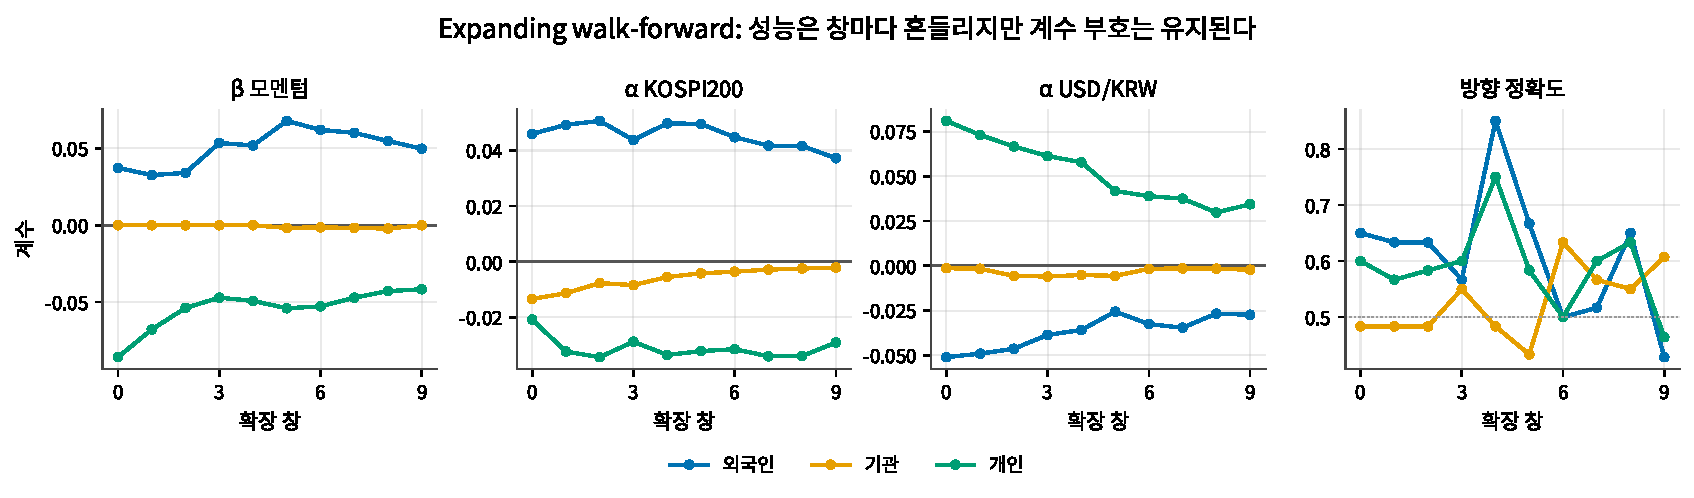
\includegraphics[width=\textwidth]{figures/fig_walk_forward.pdf}
  \caption{Expanding walk-forward 10개 창의 계수 경로와 방향 정확도((F1)--(F3) 주
  사양). 성능은 창마다 흔들리지만 계수 부호는 유지되며, 외국인과 개인의 모멘텀
  경로는 한 번도 교차하지 않는다.}
  \Description{확장 창 번호를 가로축으로 하여 세 유형의 모멘텀 계수, 두 컨텍스트
  주효과, 방향 정확도를 그린 네 개의 선그래프.}
  \label{fig:walkforward}
\end{figure*}

\begin{figure*}[t]
  \centering
  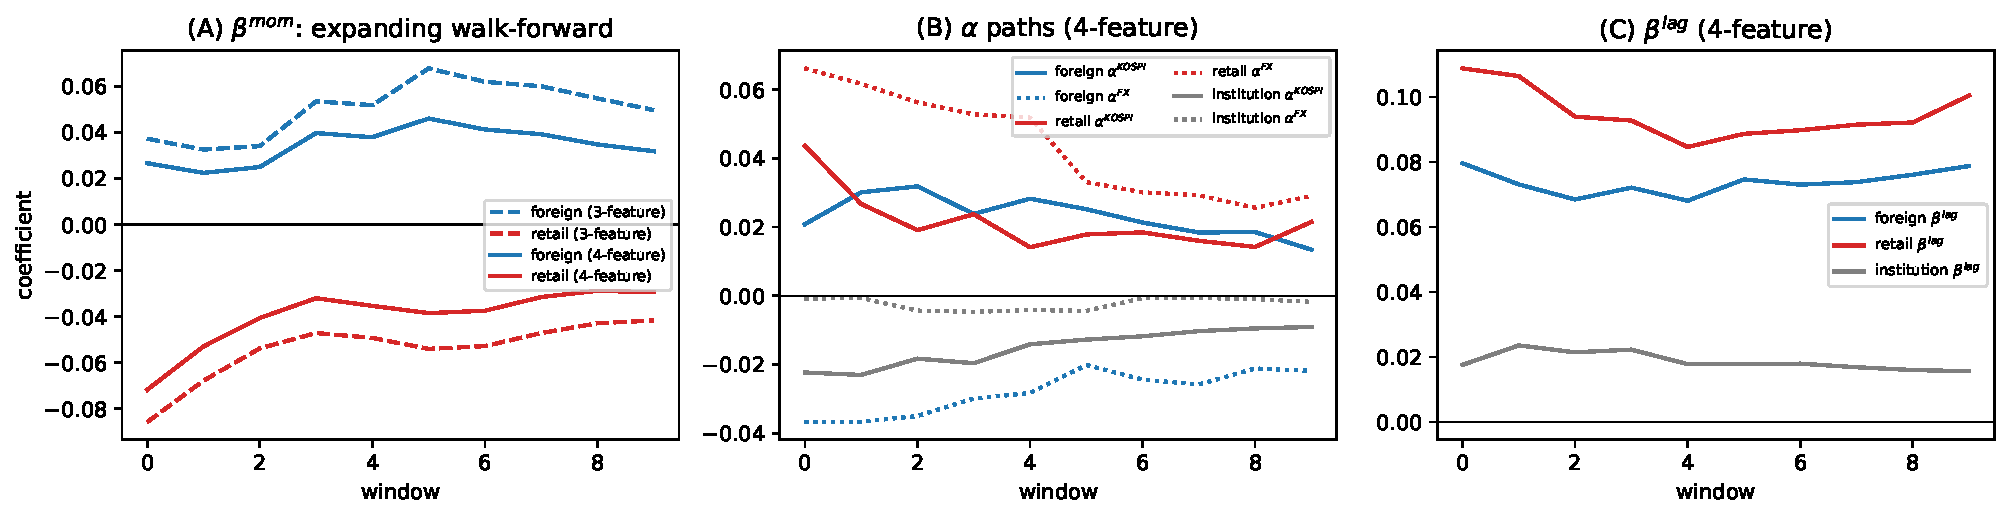
\includegraphics[width=\textwidth]{figures/fig3ext_walk_forward_4feature.pdf}
  \caption{승격 사양의 walk-forward 계수 경로(그림~\ref{fig:walkforward}의 확장).
  (A) $\beta^{mom}$: 점선은 (F1)--(F3), 실선은 승격 사양이며 두 유형의 경로가 어느
  사양에서도 교차하지 않는다. (B) 승격 사양의 $\alpha$ 경로: 개인 $\alpha^{KOSPI}$가
  10개 창 전부에서 양수다. (C) 지연 자기행동 계수 $\beta^{lag}$.}
  \Description{세 패널의 선그래프. 왼쪽 패널은 외국인과 개인의 모멘텀 계수 경로를
  3특징과 4특징 사양에 대해 각각 실선과 점선으로 보이고, 가운데 패널은 세 유형의
  KOSPI200 및 환율 주효과 경로를, 오른쪽 패널은 세 유형의 지연 자기행동 계수를
  보인다.}
  \label{fig:wf4}
\end{figure*}

\textbf{(V2)} 부트스트랩 결과는 셋으로 갈린다. 모멘텀 거울상과 컨텍스트 거울상을
이루는 8개 항이 모두 0을 제외하고, 손실구간은 통과하지 못하며, 기관은 어떤 항도
0을 제외하지 못한다(그림~\ref{fig:forest}의 속 빈 표식).

\textbf{(V3)} 그림~\ref{fig:walkforward}에서 성능은 크게 흔들린다. 외국인 방향
정확도는 0.43--0.85를 오가며 평균 $0.610\pm0.116$, 상관은 $0.131\pm0.162$로 CPCV의
0.278에서 절반 이하다. CPCV는 시험 폴드를 학습 폴드보다 앞세울 수 있는 반면
walk-forward는 그렇지 않으므로, 본 연구는 이 저하를 시간 구조에서 오는 일반화
한계로 그대로 보고한다. 반면 계수 경로는 흔들리지 않는다. 외국인 모멘텀은 10개 창
전부 양수, 개인은 전부 음수이며 두 경로가 한 번도 교차하지 않고, 두 컨텍스트
주효과에서도 같은 거울상이 유지된다. 기관의 경로는 0선에 붙어 있다.

\textbf{(V4)} 외국인과 개인의 계수는 $L_1$, $L_2$, 무벌점에서 소수점 넷째 자리까지
일치하므로 거울상은 벌점의 산물이 아니다. 반면 기관의 계수만 벌점에 따라
이동한다(시차 교차연관 $-0.0076\rightarrow-0.0124$, 손실구간
$-0.0000\rightarrow-0.0018$).

\textbf{승격 사양의 검증.} 지연 자기행동을 포함한 사양에도 V1--V4를 동일하게
적용했다(표~\ref{tab:spec34}, 그림~\ref{fig:wf4}). 모멘텀 대비와 $\alpha^{FX}$
대비는 네 검증을 모두 통과하고(walk-forward 10/10 창 부호 유지, 경로 비교차),
$\alpha^{KOSPI}$는 개인에서 10개 창 전부 양수로 반전되며, 손실구간은 약화된다.
외국인ㆍ개인 계수가 $L_1$/$L_2$/무벌점에서 소수 넷째 자리까지 일치하고 기관만
이동하는 패턴도 주 사양과 동일하다. 지연 자기행동을 컨텍스트와 상호작용시킨 확장
사양에서는 해당 상호작용 6개 항 전부의 CI가 0을 포함하며 다른 항의 변화는 0.0015
이내이므로, 본문은 파라미터 절약을 위해 $\beta$ㆍ$\alpha$만 확장한 사양을 보고한다.

\subsection{기관: 수렴된 null}
\label{sec:null}

기관 수급에 대해 SPR-IRL은 일별 빈도에서 안정적으로 식별되는 선호를 찾지 못했고,
본 연구는 이를 은폐하지 않고 결과로 보고한다. 근거는 다섯이다. (i) 예측 계열이 0선에
퇴화한다(그림~\ref{fig:prediction}). (ii) 시차 교차연관을 제외한 계수의 크기가 다른
유형보다 한 자릿수 이상 작다---현행 $\lambda$에서 $-0.0006$ㆍ$-0.0008$(약 $1/40$),
$\lambda$를 0으로 통일해도 $-0.0029$ㆍ$-0.0018$(약 $1/15$--$1/20$; 부록
표~\ref{tab:A3}). (iii) 부트스트랩에서 0을 제외하는 항이 없다(그림~\ref{fig:forest}).
(iv) 계수가 벌점 선택에 좌우된다. (v) walk-forward 10개 창에서 모멘텀 부호 일관성이
40\%, 손실구간이 0\%다.

\textbf{이 null은 최적화 실패가 아니다.} 명제~\ref{prop:lasso}에 따라 기관의 학습
인덱스에서 제약 문제~\eqref{eq:closs}은 볼록이고 그 해가 유일하다. 도달한 해와 동일
목적함수의 폐쇄형 최적해를 비교하면 기관의 목적함수 상대 격차는 평균 0.17\%, 최대
0.48\%에 불과하다(외국인 0.21\%, 개인 0.92\%). 세 유형 모두 도달 가능한 최적해에
근접했고, 기관에서만 그 최적해의 계수가 0 근방이다. 데이터가 기관에 대해 결정하는
선호가 없는 것이지 최적화가 찾지 못한 것이 아니다. 이 벌점 의존성은 계수 수준에서도
확인된다. 기관의 모멘텀ㆍ손실구간 좌표에서 목적함수 상대 격차 0.2\% 이내의 두
해---보고된 확률적 해와 폐쇄형 해---가 각각 $-0.0006$ㆍ$-0.0008$과 정확히 0(45개
분할 중 36개ㆍ44개)을 주므로, 이 좌표들에서 목적함수는 사실상 평평하며 0이 아닌
잔여값과 그로부터 계산된 부호 일관성(71\%ㆍ80\%)은 신호가 아니라 최적화
잔여물이다(부록 표~\ref{tab:A1}).

경제적으로 이 null은 투자자 분류에 대한 발견으로 읽어야 한다. ``기관''은 연기금,
투신, 보험, 사모, 금융투자를 합산한 범주다. 이 범주의 일평균 총거래금액은 958억
원으로 세 유형 중 가장 크지만 순매수 강도의 표준편차는 0.125로 가장 작다---큰
총거래가 반대 방향으로 상쇄되고 있다는 직접적 흔적이다. 상이한 목적함수를 가진 세부
주체들의 수급을 합산하면 일별 빈도에서 식별되는 공통 선호가 남지 않는다는 것이 본
결과의 내용이며, 세부 주체 분해는 \S\ref{sec:future}의 검정 가능한 가설로 남긴다.

다만 이 null은 특징 공간에 한정된다. 지연 자기행동을 통제한 승격 사양에서 기관은
$\alpha^{KOSPI}=-0.0113$(45개 분할 전부 음수, CI $[-0.0209,-0.0031]$)과 자기지연
$+0.0175$를 보이므로(표~\ref{tab:spec34}), ``어떤 항도 부트스트랩을 통과하지
못한다''는 서술은 (F1)--(F3) 주 사양에 한정해 유지한다.

\subsection{구성 타당성 점검}
\label{sec:construct}

\begin{table}[t]
  \caption{사전 부호 기대와 복원 결과}
  \label{tab:construct}
  \small
  \begin{tabular}{@{}>{\raggedright\arraybackslash}p{0.30\columnwidth}
                  >{\raggedright\arraybackslash}p{0.13\columnwidth}
                  >{\raggedright\arraybackslash}p{0.26\columnwidth}
                  >{\raggedright\arraybackslash}p{0.16\columnwidth}@{}}
    \toprule
    규칙성 & 사전 기대 & 복원 결과 & 판정 \\
    \midrule
    외국인 추세거래~\cite{grinblatt2000investment,choe1999foreign}
      & $\beta^{mom}\!>\!0$ & $+0.0496$ (100\%, CI 0 제외) & 부합 \\
    개인 역추세~\cite{grinblatt2000investment,kaniel2008individual}
      & $\beta^{mom}\!<\!0$ & $-0.0304$ (100\%, CI 0 제외) & 부합, 단 청산 유도 범위 내 \\
    처분효과~\cite{shefrin1985disposition,odean1998investors}
      & $\beta^{uw}\!>\!0$ & $+0.0293$ (100\%, CI 0 포함) & 부분 부합 \\
    기관 시차 교차연관 (참조:~\cite{lakonishok1992impact})
      & $\beta^{herd}\!>\!0$ & $-0.0044$ (100\%, CI 0 포함) & 측정 대상 상이 \\
    \bottomrule
  \end{tabular}
\end{table}

표~\ref{tab:construct}이 대조 결과다. 동일한 특징과 모형 형태를 부여하고 파라미터만
분리 학습했음에도 복원된 부호가 독립적으로 확립된 규칙성과 부합하고 두 유형이
모멘텀에서 정반대로 갈린다는 점이 구성 타당성의 증거다. 마지막 행은 측정 대상이
다르기 때문에 불일치로 보인다. Lakonishok 외~\cite{lakonishok1992impact}는 기관
\emph{내부}의 군집을, 식~\eqref{eq:herd}은 기관이 \emph{다른 두 유형}과 같은 방향으로
움직이는지를 측정하므로 본 결과는 해당 문헌의 반증이 아니다. 나아가
\S\ref{sec:beta}의 합성 실험은 음의 시차 교차연관이 선호 없이 청산 제약만으로
발생함을 보이므로, 이 항목은 구성 타당성 대조가 아니라 식별 경계의 예시로 읽는 것이
옳다.

%  의존:  sections/generated/*.tex (scripts/revision_20260727_make_tex_tables.py 산출)
% =====================================================================

\section{방법: SPR-IRL}
\label{sec:method}

본 절은 대칭 선호복원(Symmetric Preference Recovery, 이하 SPR-IRL) 절차를
정의한다. SPR-IRL은 모형 하나가 아니라 (i) 공유 특징 위의 대칭 추정, (ii) 표본외
안정성 평가, (iii) 사전 부호 기대와의 대조로 이루어진 절차다.

\subsection{연속 행동과 대칭 추정}
\label{sec:setup}

투자자 유형을 $\mathcal{I}=\{\text{외국인},\text{기관},\text{개인}\}$으로 둔다.
유형 $i$의 $t$일 총매수ㆍ총매도금액을 $V^{buy}_{i,t}$, $V^{sell}_{i,t}$라 하면
행동을
\begin{equation}
u_{i,t}=\frac{V^{buy}_{i,t}-V^{sell}_{i,t}}
             {V^{buy}_{i,t}+V^{sell}_{i,t}}\in[-1,1]
\label{eq:action}
\end{equation}
로 정의한다. 분모가 시장 전체가 아니라 해당 유형의 총거래금액이므로 $u_{i,t}$는
유형별 거래 규모에 영향받지 않는 공통 척도가 되며, 이진 라벨과 달리 강도 정보를
보존한다.

세 유형은 동일한 상태 특징 $x_{i,t}\in\mathbb{R}^{3}$, 동일한 컨텍스트
$C_t\in\mathbb{R}^{2}$, 동일한 모형 형태를 부여받고 파라미터
$\theta_i=(\beta_i,B_i,\alpha_i)$만 각자의 데이터로 분리 학습한다. 유형별로 다른
특징을 미리 배정하지 않으므로, 결과의 유형 간 차이는 설계가 아니라 데이터에서
학습된 것이며 이것이 계수의 직접 비교를 정당화한다.

학습 표본은 $(x_{i,t},C_t,a_{i,t+1})$, $a_{i,t+1}=u_{i,t+1}$이다. $t$일 상태가
$t+1$일 행동을 설명하므로 미래 거래는 특징에 들어가지 않는다.

\subsection{보상 특징과 시장 컨텍스트}
\label{sec:features}

세 특징과 두 컨텍스트는 모두 각 분할의 학습 인덱스에서만 표준화하므로, 이후 계수는
1표준편차 변화의 효과로 읽는다.

\textbf{(F1) 중기 모멘텀} $x^{mom}_{t}=\log(P_t/P_{t-20})$. 20거래일은 해석을 위한
사전 지정값이며 자료에서 최적화하지 않았다. 양수는 추세추종, 음수는 역추세를 뜻하고
부호 기대는 유형별 모멘텀 거래 문헌~\cite{grinblatt2000investment,choe1999foreign}에서
온다. 이 창과 (F3)의 망각계수 $\rho=0.98$은 사전 지정값이며,
$\rho\in\{0.95,0.98,0.99\}\times$창$\in\{10,20,60\}$의 아홉 조합 전부에서
\S\ref{sec:beta}의 모멘텀 부호 대비와 개인 손실구간 부호가 유지된다(부록
표~\ref{tab:A4}).

\textbf{(F2) 유형 간 시차 교차연관} 유형 $i$를 제외한 두 유형의 전일 행동 횡단면
평균
\begin{equation}
x^{herd}_{i,t}=\tfrac{1}{2}\left(u_{j,t-1}+u_{k,t-1}\right),\qquad j,k\neq i.
\label{eq:herd}
\end{equation}
1거래일 지연은 정보 제약이 아니라, 동일 거래일 유형 간 수급의 회계적 상쇄를 예측
변수에서 배제하기 위한 설계 선택이다(\S\ref{sec:beta}). 부호 기대는 기관 군집행동
문헌~\cite{lakonishok1992impact}을 참조하되, 해당 문헌은 기관 \emph{내부}의 군집을,
식~\eqref{eq:herd}은 \emph{유형 간} 시차 관계를 측정하므로 이 특징의 계수는
군집행동의 직접 검정이 아니다(\S\ref{sec:construct}).

\textbf{(F3) 평균단가 대비 손실구간} 평균단가 대용치 $\bar P_{i,t}$와 당일 총거래
VWAP $P^{vwap}_{i,t}$로
\begin{equation}
x^{uw}_{i,t}=\max\!\left(
\frac{\bar P_{i,t}-P^{vwap}_{i,t}}{\bar P_{i,t}},\,0\right).
\label{eq:underwater}
\end{equation}
0에서 절단하므로 이 변수는 준거점 의존적 설계다. 평균단가는 총매수ㆍ총매도 수량과
금액으로 유효 보유량을 재귀 갱신해 구하되 전일 보유량에 망각계수 $\rho=0.98$을
곱한다(반감기 약 34거래일). 부호 기대는 처분효과
문헌~\cite{shefrin1985disposition,odean1998investors}에서 온다. 다만 이 대용치는
집계 거래로 만든 근사치이므로 $x^{uw}$의 계수를 처분효과의 직접 검정으로 읽을 수
없다.

\textbf{컨텍스트}는 KOSPI200 1일 수익률 $r_t$와 원/달러 환율 수준
$z_t=(\log e_t-\mu_{t-1,252})/\sigma_{t-1,252}$이다. 평균과 표준편차는 $t-1$까지의
252거래일만 쓴다. 삼성전자의 KOSPI200 비중 때문에 종목 모멘텀과 시장수익률이
겹치며 특징--컨텍스트 상관은 $-0.29$에서 $0.22$ 범위다. 따라서 개별 계수는 다른
항이 통제된 조건부 연관이다.

\subsection{근시안적 보상과 제약 Lasso로의 환원}
\label{sec:model}

유형 $i$의 행동점수를
\begin{equation}
q_{i,t}=(\beta_i+B_iC_t)^{\top}x_{i,t}+\alpha_i^{\top}C_t
\label{eq:score}
\end{equation}
로 둔다. $\alpha$는 종목 특징이 평균일 때도 행동 수준을 옮기는 수준효과, $B$는
컨텍스트에 따라 특징 민감도가 달라지는 기울기 효과다. 상호작용을 넣으면서 하위차수
항 $C_t$를 빼는 것은 표준적 사양 오류이므로 $\alpha$의 포함은 자료로 정당화할
대상이 아니다. 연속 행동에 대한 단기 보상을
$R_i=q_{i,t}a-\tfrac{\kappa}{2}a^{2}$로 두면 최적 정책은
\begin{equation}
a^{*}_{i,t+1}=\mathrm{clip}(q_{i,t}/\kappa,-1,1)
\label{eq:policy}
\end{equation}
이다. 이차항이 없으면 해가 거의 항상 $\pm1$이 되어 행동 강도를 재현할 수 없다.
$\kappa$는 식별을 위해 1로 고정하며, 이는 보상과 계수의 단위를 고정하는 정규화이지
곡률이 경험적으로 1이라는 주장이 아니다. 학습목적은
\begin{equation}
\min_{\theta_i}\ \frac{1}{|\mathcal{D}_i|}
\sum_{t\in\mathcal{D}_i}\!\bigl(a^{*}_{i,t+1}-a_{i,t+1}\bigr)^{2}
+\lambda_i\lVert\theta_i\rVert_1
\label{eq:loss}
\end{equation}
이다. 여기서
\[
\begin{aligned}
z_{i,t}&=[\,x_{i,t};\ \mathrm{vec}(x_{i,t}C_t^{\top});\ C_t\,]\in\mathbb{R}^{11},\\
\theta_i&=[\,\beta_i;\ \mathrm{vec}(B_i);\ \alpha_i\,]
\end{aligned}
\]
로 두면 $q_{i,t}=\theta_i^{\top}z_{i,t}$이므로 식~\eqref{eq:loss}은 $z$ 위의 벌점 회귀
형태를 갖는다.

\textbf{그러나 식~\eqref{eq:loss}은 볼록이 아니다.} 예측값이 절단되기 때문이다.
한 관측의 손실을
$\ell(u)=(\mathrm{clip}(u)-a)^2$라 하자. $a=0$이면
$\ell(-2)=\ell(-1)=1$, $\ell(0)=0$이므로
$\ell(-1)$이 두 값의 평균 $0.5$를 넘어 $\ell$은 볼록이 아니다. 더구나 $\mathrm{clip}$은 상자
$[-1,1]^{n}$으로의 사영이고 관측 행동이 그 상자 안에 있으므로 모든 $\theta$에서
\[
\lVert\mathrm{clip}(Z\theta)-a\rVert\ \le\ \lVert Z\theta-a\rVert
\]
가 성립한다. 즉 포화는 오차를 줄일 수도 있으며(부록~\ref{app:convexity}의 최소 예),
어떤 해에서 $|q|<1$임을 확인하는 것만으로 포화영역에 더 좋은 해가 없다고 결론지을 수
없다.

따라서 본 논문은 추정량을 처음부터 제약 문제로 정의한다. 학습 인덱스
$\mathcal{D}_i$에 대해 $\mathcal{C}_i=\{\theta:\ |z_{i,t}^{\top}\theta|\le 1,\
\forall t\in\mathcal{D}_i\}$로 두고
\begin{equation}
\hat\theta_i=\operatorname*{arg\,min}_{\theta\in\mathcal{C}_i}\ \frac{1}{|\mathcal{D}_i|}
\sum_{t\in\mathcal{D}_i}\bigl(z_{i,t}^{\top}\theta-a_{i,t+1}\bigr)^{2}
+\lambda_i\lVert\theta\rVert_1 .
\label{eq:closs}
\end{equation}
이 제약은 계산상의 편의가 아니라 식별 제약이다. 포화영역에서는
$\theta\mapsto\mathrm{clip}(Z\theta)$가 단사가 아니어서---모든 관측이 포화된 $\theta$는
$c>1$배 해도 예측이 같다---파라미터가 식별되지 않으며, $\lambda=0$이면 그 영역의
최적해는 연속체를 이룬다. $\mathcal{C}_i$는 정책이 내부해인 영역, 곧 계수를 행동 강도의
1표준편차 효과로 읽을 수 있는 영역이다.

\begin{proposition}[제약 Lasso 환원과 유일성]
\label{prop:lasso}
(a) $\mathcal{C}_i$ 위에서 식~\eqref{eq:loss}과 식~\eqref{eq:closs}의 목적식은 동일하다.
(b) 무제약 Lasso 해 $\tilde\theta_i$가 $\mathcal{C}_i$에 속하면 $\tilde\theta_i$는
식~\eqref{eq:closs}의 전역해이며, $\mathcal{C}_i$의 \emph{내부}에 속하면 두 문제의 KKT
조건이 일치한다(제약 승수가 0). (c) 식~\eqref{eq:closs}은 볼록 다면체 위의 볼록 문제이고,
$\lambda_i=0$일 때 $\mathrm{rank}(Z_i)=p$이면, $\lambda_i>0$일 때 등상관 집합
$E=\{j:|\tfrac{2}{n}z_{j}^{\top}(a-Z\hat\theta)|=\lambda_i\}$에 대해
$\mathrm{rank}(Z_{i,E})=|E|$이면 그 해는 유일하다.
\end{proposition}

증명은 부록~\ref{app:convexity}에 있다. 본 표본에서 세 조건이 모두 성립한다. 45개
분할$\times$3유형 전부에서 학습 인덱스의 $\max_t|z_t^{\top}\hat\theta|$가 0.558을 넘지
않아 해는 $\mathcal{C}_i$의 내부에 있고, $\mathrm{rank}(Z)=11$(최악 조건수 6.86)이며,
$\lambda>0$인 두 유형에서 $\mathrm{rank}(Z_E)=|E|$다(부록 표~\ref{tab:F1}). 따라서
식~\eqref{eq:closs}의 해는 존재하고 유일하며 무제약 Lasso 해와 일치한다. 이 영역
안에서 SPR-IRL의 ``선호를 복원한다''와 ``수급을 회귀한다''는 수치적으로 구별되지
않으며, 문제가 볼록이므로 좌표하강 정확해로 직접 풀 수 있다. 본 개정에서 보고하는
모든 확장 사양은 이 정확해로 추정했다(\S\ref{sec:null}, 부록 표~\ref{tab:A1}).

무제약 문제~\eqref{eq:loss}의 전역 최적성은 이와 별개이며 본 논문은 그것을 주장하지
않는다. 다만 부록~\ref{app:convexity}는 두 가지를 보고한다. 첫째, $\hat\theta$보다 나은
목적값을 갖는 어떤 $\theta$도 학습 관측의 20.7\%(외국인)ㆍ4.2\%(기관)ㆍ40.2\%(개인)를
넘게 포화시킬 수 없다는 증명 가능한 경계. 둘째, 분할ㆍ유형당 939개, 합계 42{,}255개
시작점의 다중시작 탐색에서 더 나은 해가 하나도 발견되지 않았다는 사실이다.

이 일치는 결함이 아니라 근시안 가정의 귀결이다. 한 걸음만 내다보면 오늘의 행동이
내일 이후에 영향을 주지 않으므로, 무엇을 원하는가(보상)와 무엇을 하는가(정책)가
하나로 겹친다. 최대엔트로피 IRL~\cite{ziebart2008maximum}의
$\pi\propto\exp(R/\tau)$를 적용하면 $\pi$는 평균 $q$의 절단정규분포가 되어
점추정치가 위와 일치하므로, 이 환원은 특정 구현의 우연이 아니라 근시안ㆍ이차보상
설정 전반의 성질이다. 역강화학습 정식화의 가치는 확장 경로에 있다. 상태 동역학과
다기간 가치를 넣는 순간 보상은 정책과 갈라지고 회귀로는 도달할 수 없는 구조적
복원이 된다(\S\ref{sec:discussion}).

\subsection{검증 프로토콜}
\label{sec:protocol}

복원된 계수를 그대로 보고하지 않고 네 단계를 거친다. \textbf{(V1)} 10개 시간 폴드
중 2개를 시험으로 쓰는 조합형 정화 교차검증~\cite{lopez2018advances}으로
$\binom{10}{2}=45$개 분할을 만들고, 1일 purge와 5일 embargo를 적용하며 모든
표준화는 학습 인덱스에만 적합한다. 분할들이 관측을 공유하므로 부호 일관성은
$p$-값이 아니라 안정성 지표로만 해석한다. \textbf{(V2)} 그 한계를 보완하기 위해
표본을 달력월 블록으로 나누어 1{,}000회 복원추출하고 95\% 신뢰구간을 구한다. 월
블록은 일별 수급의 자기상관을 블록 안에 보존한다. \textbf{(V3)} CPCV는 시험 폴드가
학습 폴드보다 앞설 수 있으므로, 최초 400개 관측에서 시작해 5일 purge 후 다음
60거래일을 예측하고 학습 구간을 60거래일씩 넓히는 expanding walk-forward를 10개 창
수행한다. \textbf{(V4)} 결과가 $L_1$ 벌점의 산물이 아님을 보이기 위해 $L_2$ 및
무벌점으로 재추정해 부호를 비교한다.

지표는 MAE, RMSE, 방향 정확도($\mathrm{sign}(a^{*})=\mathrm{sign}(a)$의 비율),
예측--실제 상관, 포화 비율이다. 유형 간 행동 표준편차가 다르므로 오차의 절대값은
유형 간 비교에 쓰지 않는다. 자명한 참조로 전일 자기행동을 그대로 예측하는 지속성
규칙을 함께 보고한다.

% =====================================================================
\section{실험}
\label{sec:experiments}

\subsection{데이터}
\label{sec:data}

삼성전자(005930) 일별 자료에서 252일 환율 이력, 20일 모멘텀, 다음 날 행동을 모두
계산할 수 있는 최신 973행을 사용한다. 상태일은 2022-01-06--2025-12-29이다. 단일
종목은 표본의 한계가 아니라 종목 고정효과와 유동성 차이를 배제하고 유형 간 선호
이질성만 분리하기 위한 통제된 설정이다.

행동 평균은 세 유형 모두 0에 가깝지만 표준편차는 개인 0.334, 외국인 0.257, 기관
0.125로 다르고, 1차 자기상관은 각각 0.345, 0.401, 0.149다. 동일 거래일 유형 간
행동은 강한 음의 관계를 갖는다(외국인--개인 $-0.772$, 기관--개인 $-0.499$). 이 음의
동시점 구조가 유형 간 계수 해석에 부과하는 식별 경계는 \S\ref{sec:beta}에서
정량화한다. 세 유형 순매수 합계와 시장 전체의 차이(기타법인ㆍ기타외국인 등)는
일평균 144억 원, 거래대금의 1.3\%에 그친다.

학습 설정은 유형별로 외국인 75 epochs / batch 256 / lr 0.001 / $\lambda=0$, 기관
10 / 2048 / 0.0005 / 0.01, 개인 20 / 512 / 0.001 / 0.0003이며 seed 42, $\kappa=1$,
유형당 파라미터 11개($\beta$ 3, $B$ 6, $\alpha$ 2)다. 유형별 $\lambda$는 본
사양에서 중첩 교차검증으로 선택된 값이 아니라, 선행 이산행동 사양에서 CPCV 정확도
그리드 탐색으로 정해져 이월된 값이다. 따라서 $\lambda$ 비대칭이 결과를 만드는지
확인하기 위해 세 유형에 동일한 $\lambda\in\{0,0.0005,0.01\}$을 부여한 재추정을 부록
표~\ref{tab:A3}에 함께 보고하며, 거울상 부호는 모든 $\lambda$ 사양에서 유지된다.

\subsection{표본외 행동 재현}
\label{sec:oos}

\begin{figure}[t]
  \centering
  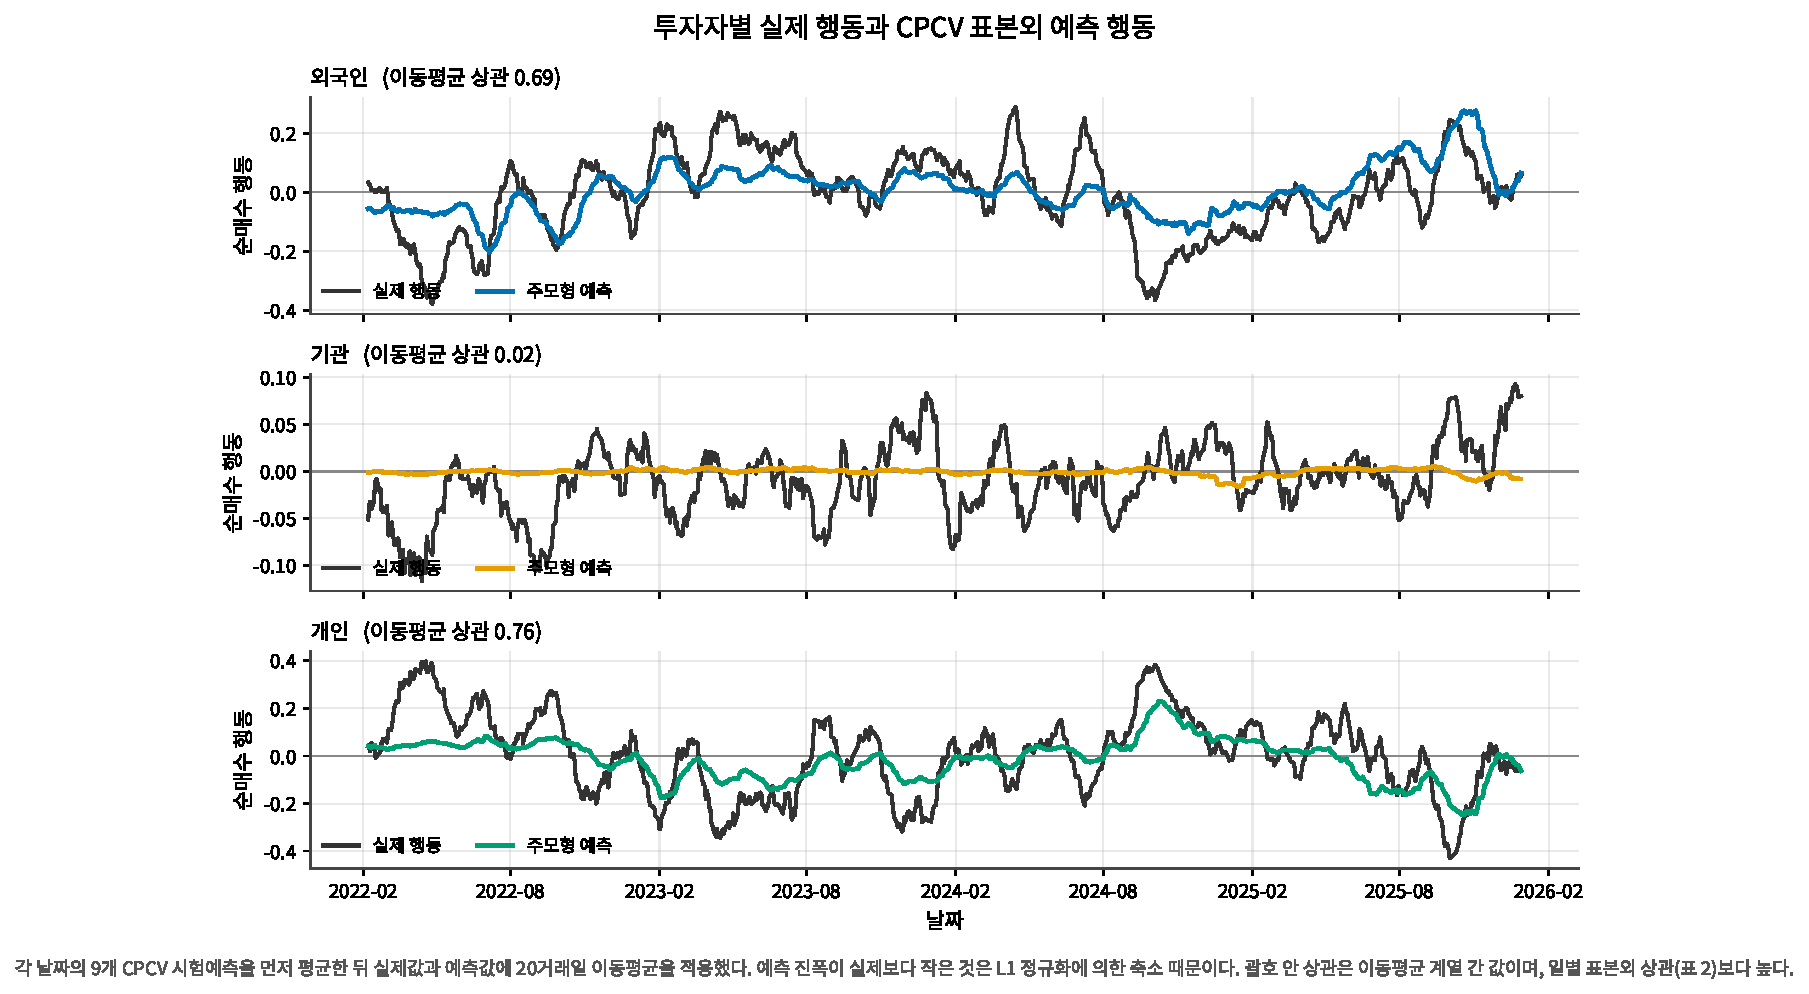
\includegraphics[width=\columnwidth]{figures/fig_actual_vs_prediction.pdf}
  \caption{실제 행동과 CPCV 표본외 예측(20거래일 이동평균). 각 날짜의 9개 시험예측을
  먼저 평균했다. 괄호 안은 평활 계열 간 상관으로,
  표~\ref{tab:performance}의 일별 상관과 직접 비교하지 않는다.}
  \Description{외국인, 기관, 개인의 실제 순매수와 모형 예측을 시간축에 겹쳐 그린
  세 개의 선그래프. 기관 패널에서 예측선이 0 근방에 평탄하게 놓여 있다.}
  \label{fig:prediction}
\end{figure}

\begin{table}[t]
  \caption{CPCV 표본외 성능(45개 분할 평균 $\pm$ 표준편차), 지속성 기준선, 그리고
  지연 자기행동을 포함한 승격 사양}
  \label{tab:performance}
  \small
  \centering
  \begin{tabular}{@{}lccc@{}}
    \toprule
    지표 & 외국인 & 기관 & 개인 \\
    \midrule
    \multicolumn{4}{@{}l}{\emph{SPR-IRL} (F1)--(F3), 주 사양}\\
    방향 정확도 & $0.636\pm0.039$ & $0.542\pm0.038$ & $0.608\pm0.044$ \\
    상관계수    & $0.278\pm0.110$ & $0.068\pm0.064$ & $0.245\pm0.118$ \\
    MAE         & $0.195\pm0.019$ & $0.094\pm0.008$ & $0.264\pm0.029$ \\
    MAE / 행동 SD & $0.759$ & $0.756$ & $0.791$ \\
    포화 비율   & $0.000$ & $0.000$ & $0.000$ \\
    \addlinespace
    \multicolumn{4}{@{}l}{\emph{지속성 기준선} ($a_{t+1}\!\leftarrow\!a_t$)}\\
    방향 정확도 & $0.642$ & $0.547$ & $0.616$ \\
    상관계수    & $0.359$ & $0.136$ & $0.311$ \\
    \addlinespace
    \multicolumn{4}{@{}l}{\emph{승격 사양} (F1)--(F3)$+u_{i,t}$, 정확해 (\S\ref{sec:beta})}\\
    \inputrows{sections/generated/tab1_rows.tex}
    \bottomrule
  \end{tabular}
\end{table}

그림~\ref{fig:prediction}에서 외국인과 개인의 예측 계열은 실제 계열의 국면 전환을
따라가지만(평활 상관 0.69, 0.76) 진폭은 작다. 이는 벌점의 산물이 아니라---외국인은
$\lambda=0$이다---설명력이 유한한 회귀의 조건부 기대가 갖는 일반적 성질이다. 표본외
$R^2$가 0.10--0.18인 예측치의 표준편차는 실제 행동 표준편차의 1/3 수준으로
축소된다. 기관의 예측 계열은 사실상 0선에 붙어 있다(0.02).

표~\ref{tab:performance}에서 세 가지가 드러난다. 첫째, 분할 간 산포가 커서 단일
분할의 수치로 유형을 비교할 수 없다. 둘째, 자명한 지속성 기준선이 방향 정확도와
상관계수에서 (F1)--(F3) 사양의 SPR-IRL을 앞선다. $a_t$는 $t$일 종가 이후 공개되므로
이는 정보상 이용 가능한 규칙이다. 셋째, 원인은 특징 집합의 설계에 있다. 행동의
자기상관이 $0.401/0.149/0.345$인데 (F1)--(F3)에는 자기 지연행동이 없다. 이 제한은
세 유형이 독립적으로 확립된 규칙성에 대응하는 특징만 공유하도록 한 선택이지 예측
성능을 위한 설계가 아니다. \textbf{지연 자기행동 $u_{i,t}$를 네 번째 특징으로 넣은
승격 사양은 세 유형 모두에서 지속성 기준선을 넘어서며(방향 정확도 $0.652/0.574/
0.629$, 표~\ref{tab:performance}), 이때 어떤 계수 부호가 살아남는지가
\S\ref{sec:beta}의 해석을 결정한다(표~\ref{tab:spec34}).} 즉 선호 복원과 수급
예측은 상이한 특징 집합을 요구하는 별개의 과제다.

모든 유형ㆍ모든 분할에서 학습 인덱스의 포화 비율이 0이므로 명제~\ref{prop:lasso}(b)의
전제가 성립하고, 제약 추정량~\eqref{eq:closs}은 무제약 Lasso와 일치한다. 승격 사양에서도
포화 비율은 45개 분할 전부 0이며 표본 전체에서 $|q|$의 최대값은 0.959다.

\subsection{복원된 구조: 모멘텀 축의 거울상과 그 식별 경계}
\label{sec:beta}

\begin{figure*}[t]
  \centering
  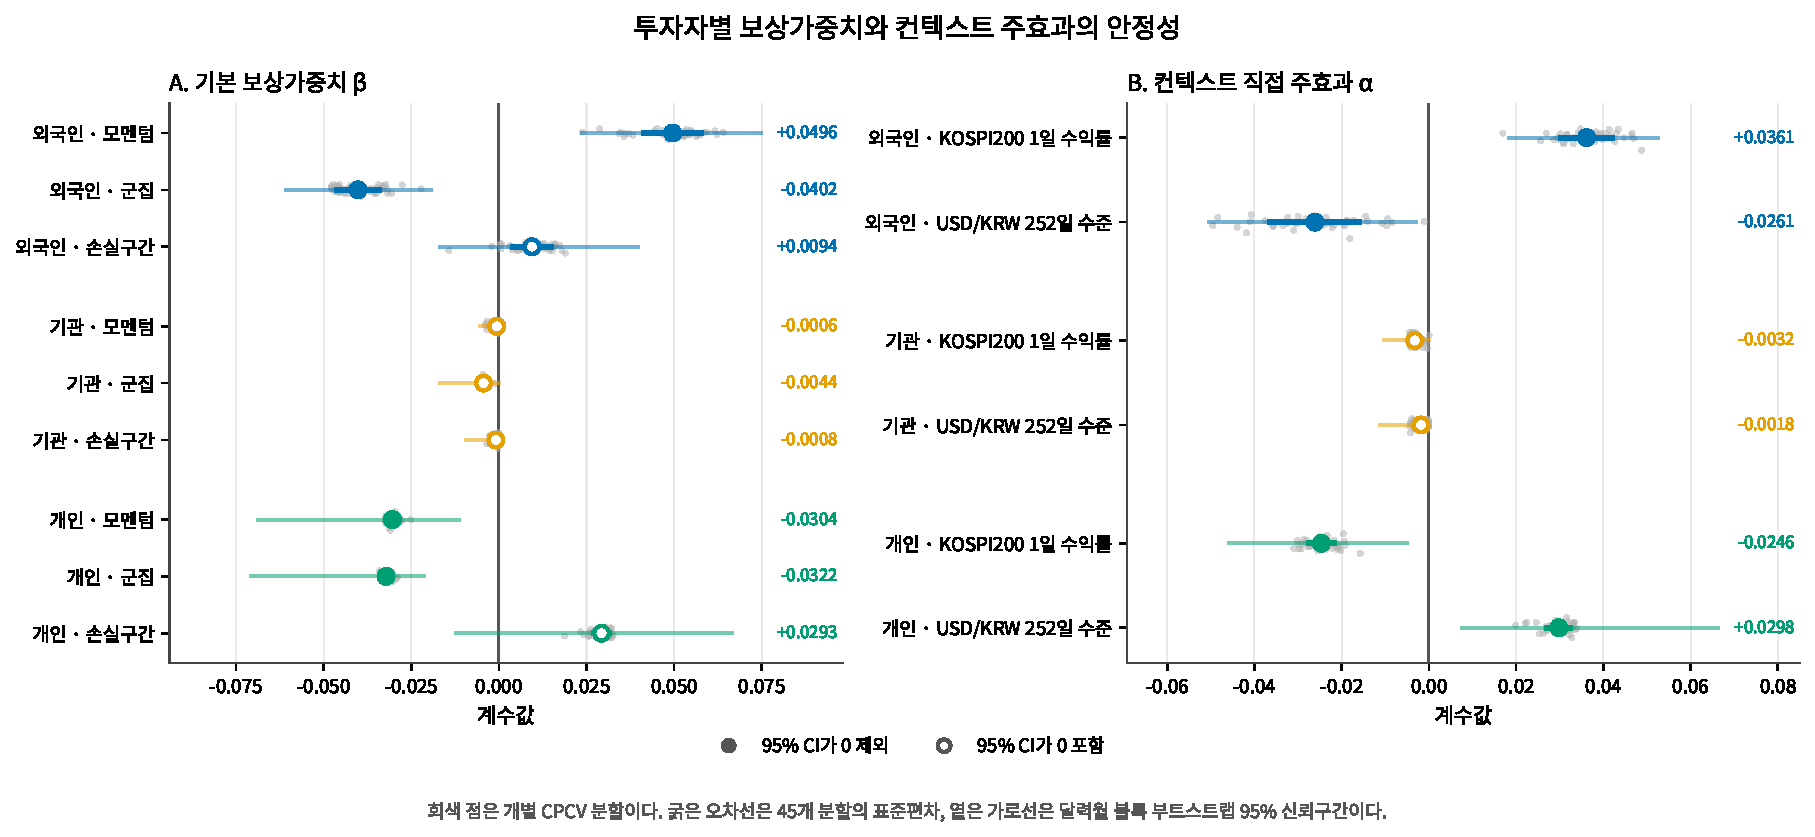
\includegraphics[width=\textwidth]{figures/fig_beta_alpha_forest.pdf}
  \caption{복원된 기본 보상가중치 $\beta$(A)와 컨텍스트 주효과 $\alpha$(B)의 안정성.
  회색 점은 45개 개별 CPCV 분할, 굵은 오차선은 분할 간 표준편차, 옅은 가로선은 달력월
  블록 부트스트랩 95\% 신뢰구간이다. 속이 빈 표식은 신뢰구간이 0을 포함하는 항이다.}
  \Description{두 패널의 forest plot. 패널 A는 세 유형의 모멘텀, 시차 교차연관,
  손실구간 계수를, 패널 B는 KOSPI200과 환율 주효과를 보인다. 외국인 모멘텀은 양,
  개인 모멘텀은 음이며 기관의 모든 표식은 속이 비어 있다.}
  \label{fig:forest}
\end{figure*}

\begin{table*}[t]
  \caption{(F1)--(F3) 주 사양과 지연 자기행동을 포함한 승격 사양의 계수 대조.
  값은 정확해 CPCV 45개 분할 평균, 괄호는 부호 일관성, CI는 달력월 블록 부트스트랩
  1{,}000회의 95\% 신뢰구간이며 $^{*}$는 0을 제외함을 뜻한다. 주 표(표~\ref{tab:performance},
  그림~\ref{fig:forest})의 Adam 수치는 변경하지 않았다.}
  \label{tab:spec34}
  \small
  \centering
  \begin{tabular}{@{}llcccc>{\raggedright\arraybackslash}p{0.14\textwidth}@{}}
    \toprule
    유형 & 항 & (F1)--(F3) 평균 & CI & 승격 사양 평균 & CI & 판정 \\
    \midrule
    \inputrows{sections/generated/tab3_body.tex}
    \bottomrule
  \end{tabular}
\end{table*}

\textbf{청산 제약이 정하는 해석의 경계.} 유형 간 계수를 비교하기 전에, 시장 청산이
기계적으로 만들 수 있는 것부터 정량화한다. 본 표본에서 외국인 순매수 1원은 평균적으로
개인 $-0.92$원, 기관 $-0.06$원, 기타 $-0.02$원으로 흡수되고, 유형별 총거래금액
비율은 $\mathbb{E}[W_{f}/W_{r}]=1.21\text{--}1.42$다. 따라서 외국인이 표준화 특징
$x$에 $\beta_f$만큼 반응하면, 개인이 아무 선호가 없어도 개인 계수에는
$\beta_{r}^{ind}\approx-0.92\times\beta_f\times(1.21\text{--}1.42)$의 성분이
유도된다(유도 과정과 가정은 부록~\ref{app:derivation}). 관측된 외국인 계수를 대입한
유도 성분은 \textbf{관측된 개인 계수를 전 항목에서 초과하거나 근사한다(관측의
84--214\%; 부록 표~\ref{tab:A2})}. 외국인만 선호를 갖는 합성 세계 1{,}000회의 전체
파이프라인 추정도 같은 결론을 준다. 개인이 물려받는 $\beta^{mom}$ 분포는
$[-0.101,-0.015]$로 관측치를 내부에 품으며, 이 세계는 동시점 상관 $-0.74$(관측
$-0.77$)와 기관의 null까지 재현한다. 반대로 선호가 전혀 없는 합성 세계에서
$\beta^{mom}$과 $\alpha$의 95\% 대역은 $\pm0.04$ 이내이므로 외국인의 $+0.0496$은 그
대역 밖(약 4.3 표준편차)에 있다. 이 두 사실이 본 절의 서술 규칙을 정한다. 유형별
계수 중 기계 대역을 초과하는 것만 선호로 읽고, 유도 범위 안의 것은 집계 수급의
구조로 읽는다.

\textbf{모멘텀 축의 거울상.} 외국인의 모멘텀 가중치는 $+0.0496$으로 45개 분할
전부에서 양수, 개인은 $-0.0304$로 전부에서 음수이며 두 부트스트랩 신뢰구간은 서로
겹치지 않고 각각 0을 제외한다(그림~\ref{fig:forest}A). 이 대비는 지연 자기행동을
통제한 승격 사양에서도 그대로 살아남는다(외국인 $+0.0331$, CI $[+0.0126,+0.0522]$;
개인 $-0.0261$, CI $[-0.0519,-0.0007]$; 표~\ref{tab:spec34}). walk-forward 10개
창에서 두 경로가 한 번도 교차하지 않으며(그림~\ref{fig:wf4}A), 벌점 종류와
$\lambda$ 통일에도 불변이다(부록 표~\ref{tab:A3}). 해석은 비대칭적이다. 외국인의
양수는 무선호 합성 대역 밖이고 자기상관ㆍ청산 통제를 모두 통과하므로 추세추종
선호로 읽으며, 이는 외국인 추세거래
문헌~\cite{grinblatt2000investment,choe1999foreign}과 부합한다. 개인의 음수는
부호와 안정성이 같은 검증을 통과하지만 크기가 청산 유도 범위 안에 있으므로,
독립적 역추세 선호의 증거로 읽지 않고 \emph{외국인의 추세거래가 청산 제약을 통해
개인 집계 수급에 남기는 반대 부호}까지만 주장한다. 개인 고유의 역추세 성향이 있는지는
이 자료의 집계 수준에서 식별되지 않는다.

\textbf{컨텍스트 주효과: 서술적 결과로 격하.} 주 사양의 $\alpha$ 네 계수(외국인
$+0.0361$/$-0.0261$, 개인 $-0.0246$/$+0.0298$)는 45개 분할 전부에서 부호가 유지되고
신뢰구간이 0을 제외한다(그림~\ref{fig:forest}B). 그러나 두 가지 이유로 본 연구는
이를 선호의 거울상이 아니라 ``관측된 집계 수급의 음의 교차 연관''이라는 서술적
결과로 제한한다. 첫째, 유도 성분이 관측을 초과한다(부록 표~\ref{tab:A2}). 둘째,
$\alpha^{KOSPI}$는 지연 자기행동을 통제하면 개인에서 $+0.0274$(45개 분할 전부 양수,
CI $[+0.0039,+0.0532]$)로 \textbf{부호가 반전}되고 외국인에서 $+0.0128$로 축소되어
CI가 0을 포함한다(표~\ref{tab:spec34}). 즉 주 사양의 개인 음수 $\alpha^{KOSPI}$는
개인 수급의 자기상관을 $\alpha$가 대신 흡수한 결과였다. $\alpha^{FX}$의 대비(외국인
$-0.0217$, 개인 $+0.0303$)만이 통제 후에도 CI를 유지하는 컨텍스트 결과다.

\textbf{유형 간 시차 교차연관.} 이 계수는 세 유형 모두 45개 분할 전부에서 음수이고
외국인($-0.0402$)과 개인($-0.0322$)은 신뢰구간도 0을 제외한다. 그러나 선호가 전혀
없는 합성 수급에서도 이 계수는 외국인 $[-0.057,-0.018]$, 개인 $[-0.085,-0.011]$로
음수가 되며 관측치는 두 대역의 내부에 있다(부록 표~\ref{tab:A2b}). 따라서 음의 시차
교차연관은 행동적 해석 없이 청산 제약과 자기상관만으로 발생 가능한 크기이며, 본
연구는 이를 서술적 결과로만 보고한다.

\textbf{손실구간.} 개인의 손실구간 가중치는 $+0.0293$으로 45개 분할 전부에서
양수이며 처분효과 문헌~\cite{shefrin1985disposition,odean1998investors}의 기준가격
의존성과 정합한다. 그러나 그림~\ref{fig:forest}A에서 보듯 세 유형 모두 신뢰구간이
0을 포함한다. 개인의 구간은 $[-0.0122,+0.0665]$로, 45개 분할에서 부호가 100\%
일관됨에도 월 블록 재표집에서는 5.5\%가 부호를 뒤집으며, 지연 자기행동을 통제하면
$+0.0115$(77.8\%)로 더 약해진다(표~\ref{tab:spec34}). 이는 CPCV 분할이 관측을
공유하기 때문에 부호 일관성이 불확실성을 과소평가한다는 \S\ref{sec:protocol}의
경고가 실제로 작동한 사례다. 따라서 처분효과와 정합하는 부호를 관측했다고 보고하되
통계적으로 확립된 결과로 주장하지 않는다.

\textbf{상호작용.} $B$ 12개는 동시에 검토한 탐색적 항목이다. 정확해 기준으로 45개
분할 부호가 유지되고 부트스트랩을 통과하는 항은 외국인
모멘텀$\times$KOSPI200($-0.0141$)과 개인 손실구간$\times$환율($-0.0408$)이다. Adam
해에서 100\% 일관으로 보였던 개인 모멘텀$\times$환율($+0.0144$)은 정확해에서
$-0.0106$(음수 91.1\%)으로 뒤집히므로 목록에서 제외한다(부록 표~\ref{tab:A1}).

\subsection{안정성}
\label{sec:stability}

\begin{figure*}[t]
  \centering
  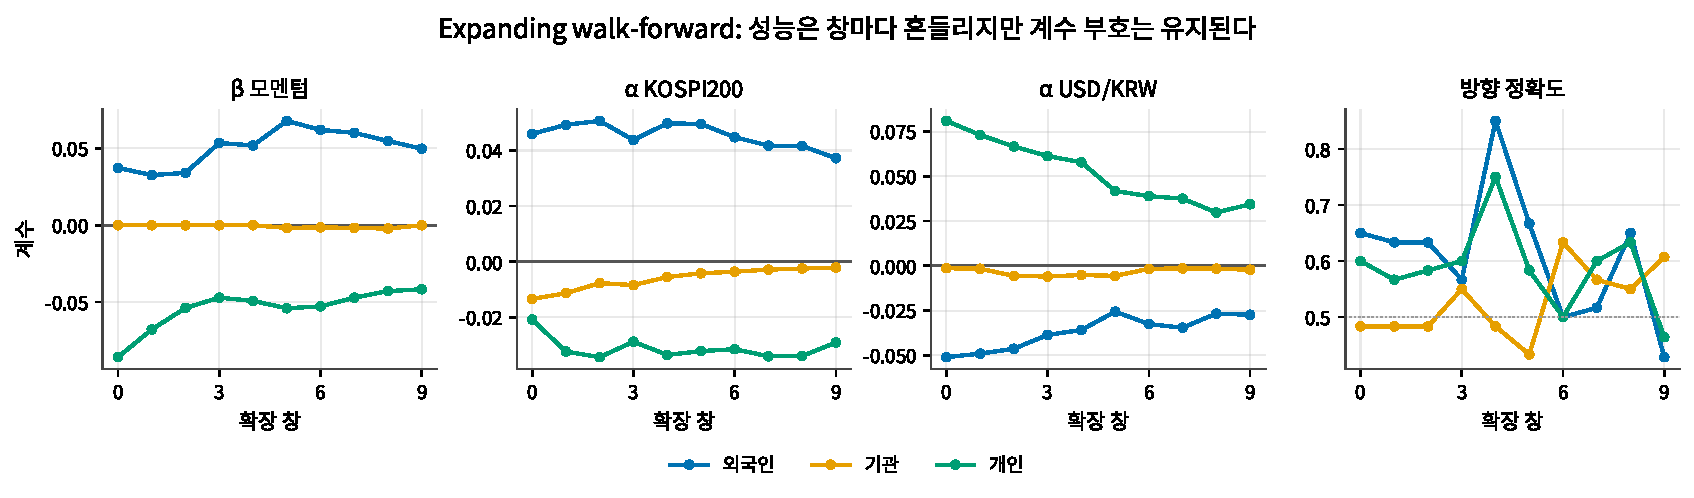
\includegraphics[width=\textwidth]{figures/fig_walk_forward.pdf}
  \caption{Expanding walk-forward 10개 창의 계수 경로와 방향 정확도((F1)--(F3) 주
  사양). 성능은 창마다 흔들리지만 계수 부호는 유지되며, 외국인과 개인의 모멘텀
  경로는 한 번도 교차하지 않는다.}
  \Description{확장 창 번호를 가로축으로 하여 세 유형의 모멘텀 계수, 두 컨텍스트
  주효과, 방향 정확도를 그린 네 개의 선그래프.}
  \label{fig:walkforward}
\end{figure*}

\begin{figure*}[t]
  \centering
  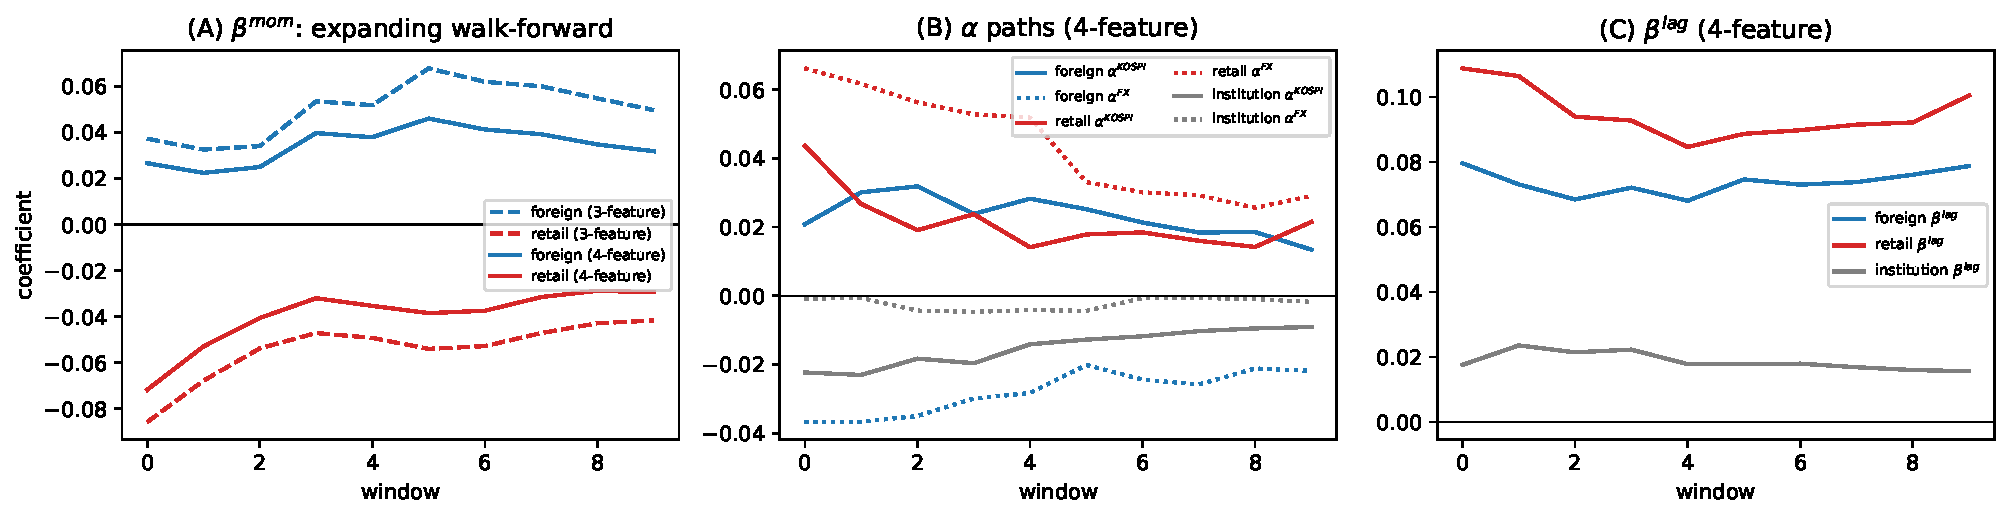
\includegraphics[width=\textwidth]{figures/fig3ext_walk_forward_4feature.pdf}
  \caption{승격 사양의 walk-forward 계수 경로(그림~\ref{fig:walkforward}의 확장).
  (A) $\beta^{mom}$: 점선은 (F1)--(F3), 실선은 승격 사양이며 두 유형의 경로가 어느
  사양에서도 교차하지 않는다. (B) 승격 사양의 $\alpha$ 경로: 개인 $\alpha^{KOSPI}$가
  10개 창 전부에서 양수다. (C) 지연 자기행동 계수 $\beta^{lag}$.}
  \Description{세 패널의 선그래프. 왼쪽 패널은 외국인과 개인의 모멘텀 계수 경로를
  3특징과 4특징 사양에 대해 각각 실선과 점선으로 보이고, 가운데 패널은 세 유형의
  KOSPI200 및 환율 주효과 경로를, 오른쪽 패널은 세 유형의 지연 자기행동 계수를
  보인다.}
  \label{fig:wf4}
\end{figure*}

\textbf{(V2)} 부트스트랩 결과는 셋으로 갈린다. 모멘텀 거울상과 컨텍스트 거울상을
이루는 8개 항이 모두 0을 제외하고, 손실구간은 통과하지 못하며, 기관은 어떤 항도
0을 제외하지 못한다(그림~\ref{fig:forest}의 속 빈 표식).

\textbf{(V3)} 그림~\ref{fig:walkforward}에서 성능은 크게 흔들린다. 외국인 방향
정확도는 0.43--0.85를 오가며 평균 $0.610\pm0.116$, 상관은 $0.131\pm0.162$로 CPCV의
0.278에서 절반 이하다. CPCV는 시험 폴드를 학습 폴드보다 앞세울 수 있는 반면
walk-forward는 그렇지 않으므로, 본 연구는 이 저하를 시간 구조에서 오는 일반화
한계로 그대로 보고한다. 반면 계수 경로는 흔들리지 않는다. 외국인 모멘텀은 10개 창
전부 양수, 개인은 전부 음수이며 두 경로가 한 번도 교차하지 않고, 두 컨텍스트
주효과에서도 같은 거울상이 유지된다. 기관의 경로는 0선에 붙어 있다.

\textbf{(V4)} 외국인과 개인의 계수는 $L_1$, $L_2$, 무벌점에서 소수점 넷째 자리까지
일치하므로 거울상은 벌점의 산물이 아니다. 반면 기관의 계수만 벌점에 따라
이동한다(시차 교차연관 $-0.0076\rightarrow-0.0124$, 손실구간
$-0.0000\rightarrow-0.0018$).

\textbf{승격 사양의 검증.} 지연 자기행동을 포함한 사양에도 V1--V4를 동일하게
적용했다(표~\ref{tab:spec34}, 그림~\ref{fig:wf4}). 모멘텀 대비와 $\alpha^{FX}$
대비는 네 검증을 모두 통과하고(walk-forward 10/10 창 부호 유지, 경로 비교차),
$\alpha^{KOSPI}$는 개인에서 10개 창 전부 양수로 반전되며, 손실구간은 약화된다.
외국인ㆍ개인 계수가 $L_1$/$L_2$/무벌점에서 소수 넷째 자리까지 일치하고 기관만
이동하는 패턴도 주 사양과 동일하다. 지연 자기행동을 컨텍스트와 상호작용시킨 확장
사양에서는 해당 상호작용 6개 항 전부의 CI가 0을 포함하며 다른 항의 변화는 0.0015
이내이므로, 본문은 파라미터 절약을 위해 $\beta$ㆍ$\alpha$만 확장한 사양을 보고한다.

\subsection{기관: 수렴된 null}
\label{sec:null}

기관 수급에 대해 SPR-IRL은 일별 빈도에서 안정적으로 식별되는 선호를 찾지 못했고,
본 연구는 이를 은폐하지 않고 결과로 보고한다. 근거는 다섯이다. (i) 예측 계열이 0선에
퇴화한다(그림~\ref{fig:prediction}). (ii) 시차 교차연관을 제외한 계수의 크기가 다른
유형보다 한 자릿수 이상 작다---현행 $\lambda$에서 $-0.0006$ㆍ$-0.0008$(약 $1/40$),
$\lambda$를 0으로 통일해도 $-0.0029$ㆍ$-0.0018$(약 $1/15$--$1/20$; 부록
표~\ref{tab:A3}). (iii) 부트스트랩에서 0을 제외하는 항이 없다(그림~\ref{fig:forest}).
(iv) 계수가 벌점 선택에 좌우된다. (v) walk-forward 10개 창에서 모멘텀 부호 일관성이
40\%, 손실구간이 0\%다.

\textbf{이 null은 최적화 실패가 아니다.} 명제~\ref{prop:lasso}에 따라 기관의 학습
인덱스에서 제약 문제~\eqref{eq:closs}은 볼록이고 그 해가 유일하다. 도달한 해와 동일
목적함수의 폐쇄형 최적해를 비교하면 기관의 목적함수 상대 격차는 평균 0.17\%, 최대
0.48\%에 불과하다(외국인 0.21\%, 개인 0.92\%). 세 유형 모두 도달 가능한 최적해에
근접했고, 기관에서만 그 최적해의 계수가 0 근방이다. 데이터가 기관에 대해 결정하는
선호가 없는 것이지 최적화가 찾지 못한 것이 아니다. 이 벌점 의존성은 계수 수준에서도
확인된다. 기관의 모멘텀ㆍ손실구간 좌표에서 목적함수 상대 격차 0.2\% 이내의 두
해---보고된 확률적 해와 폐쇄형 해---가 각각 $-0.0006$ㆍ$-0.0008$과 정확히 0(45개
분할 중 36개ㆍ44개)을 주므로, 이 좌표들에서 목적함수는 사실상 평평하며 0이 아닌
잔여값과 그로부터 계산된 부호 일관성(71\%ㆍ80\%)은 신호가 아니라 최적화
잔여물이다(부록 표~\ref{tab:A1}).

경제적으로 이 null은 투자자 분류에 대한 발견으로 읽어야 한다. ``기관''은 연기금,
투신, 보험, 사모, 금융투자를 합산한 범주다. 이 범주의 일평균 총거래금액은 958억
원으로 세 유형 중 가장 크지만 순매수 강도의 표준편차는 0.125로 가장 작다---큰
총거래가 반대 방향으로 상쇄되고 있다는 직접적 흔적이다. 상이한 목적함수를 가진 세부
주체들의 수급을 합산하면 일별 빈도에서 식별되는 공통 선호가 남지 않는다는 것이 본
결과의 내용이며, 세부 주체 분해는 \S\ref{sec:future}의 검정 가능한 가설로 남긴다.

다만 이 null은 특징 공간에 한정된다. 지연 자기행동을 통제한 승격 사양에서 기관은
$\alpha^{KOSPI}=-0.0113$(45개 분할 전부 음수, CI $[-0.0209,-0.0031]$)과 자기지연
$+0.0175$를 보이므로(표~\ref{tab:spec34}), ``어떤 항도 부트스트랩을 통과하지
못한다''는 서술은 (F1)--(F3) 주 사양에 한정해 유지한다.

\subsection{구성 타당성 점검}
\label{sec:construct}

\begin{table}[t]
  \caption{사전 부호 기대와 복원 결과}
  \label{tab:construct}
  \small
  \begin{tabular}{@{}>{\raggedright\arraybackslash}p{0.30\columnwidth}
                  >{\raggedright\arraybackslash}p{0.13\columnwidth}
                  >{\raggedright\arraybackslash}p{0.26\columnwidth}
                  >{\raggedright\arraybackslash}p{0.16\columnwidth}@{}}
    \toprule
    규칙성 & 사전 기대 & 복원 결과 & 판정 \\
    \midrule
    외국인 추세거래~\cite{grinblatt2000investment,choe1999foreign}
      & $\beta^{mom}\!>\!0$ & $+0.0496$ (100\%, CI 0 제외) & 부합 \\
    개인 역추세~\cite{grinblatt2000investment,kaniel2008individual}
      & $\beta^{mom}\!<\!0$ & $-0.0304$ (100\%, CI 0 제외) & 부합, 단 청산 유도 범위 내 \\
    처분효과~\cite{shefrin1985disposition,odean1998investors}
      & $\beta^{uw}\!>\!0$ & $+0.0293$ (100\%, CI 0 포함) & 부분 부합 \\
    기관 시차 교차연관 (참조:~\cite{lakonishok1992impact})
      & $\beta^{herd}\!>\!0$ & $-0.0044$ (100\%, CI 0 포함) & 측정 대상 상이 \\
    \bottomrule
  \end{tabular}
\end{table}

표~\ref{tab:construct}이 대조 결과다. 동일한 특징과 모형 형태를 부여하고 파라미터만
분리 학습했음에도 복원된 부호가 독립적으로 확립된 규칙성과 부합하고 두 유형이
모멘텀에서 정반대로 갈린다는 점이 구성 타당성의 증거다. 마지막 행은 측정 대상이
다르기 때문에 불일치로 보인다. Lakonishok 외~\cite{lakonishok1992impact}는 기관
\emph{내부}의 군집을, 식~\eqref{eq:herd}은 기관이 \emph{다른 두 유형}과 같은 방향으로
움직이는지를 측정하므로 본 결과는 해당 문헌의 반증이 아니다. 나아가
\S\ref{sec:beta}의 합성 실험은 음의 시차 교차연관이 선호 없이 청산 제약만으로
발생함을 보이므로, 이 항목은 구성 타당성 대조가 아니라 식별 경계의 예시로 읽는 것이
옳다.
